\pagebreak
\subsection{1D NetCDF GLOBAL\_MEAN\_ATM\_SURFACE\_PRES}
\newp
\begin{longtable}{|p{0.1\textwidth}|p{0.5\textwidth}|}
\caption{Variables in the dataset GLOBAL\_MEAN\_ATM\_SURFACE\_PRES}
\label{tab:table-GLOBAL_MEAN_ATM_SURFACE_PRES-fields} \\ 
\hline \endhead \hline \endfoot
\rowcolor{lightgray} \textbf{Dataset:} & \textbf{GLOBAL\_MEAN\_ATM\_SURFACE\_PRES} \\ \hline
Field: &Pa\_global \\ \hline
\end{longtable}

\pagebreak
\subsubsection{1D Variable Pa\_global}
\begin{longtable}{|m{0.06\textwidth}|m{0.41\textwidth}|m{0.39\textwidth}|m{0.06\textwidth}|}
\caption{CDL description of GLOBAL\_MEAN\_ATM\_SURFACE\_PRES's Pa\_global variable}
\label{tab:table-GLOBAL_MEAN_ATM_SURFACE_PRES_Pa_global} \\ 
\hline \endhead \hline \endfoot
\rowcolor{lightgray} \textbf{Storage Type} & \textbf{Variable Name} & \textbf{Description} & \textbf{Unit} \\ \hline
float64 & Pa\_global & Global mean atmospheric surface pressure over the ocean and sea-ice & N m-2 \\ \hline
\rowcolor{lightgray}  \multicolumn{4}{|p{1.00\textwidth}|}{\textbf{CDL Description}} \\ \hline
\multicolumn{4}{|p{1.00\textwidth}|}{\makecell{\parbox{1\textwidth}{float64 Pa\_global(time)\\
\hspace*{0.5cm}Pa\_global: \_FillValue = 9.969209968386869e+36\\
\hspace*{0.5cm}Pa\_global: coverage\_content\_type = modelResult\\
\hspace*{0.5cm}Pa\_global: long\_name = Global mean atmospheric surface pressure over the ocean and sea: ice\\
\hspace*{0.5cm}Pa\_global: standard\_name = air\_pressure\_at\_sea\_level\\
\hspace*{0.5cm}Pa\_global: units = N m: 2\\
\hspace*{0.5cm}Pa\_global: valid\_min = 100873.14755283327\\
\hspace*{0.5cm}Pa\_global: valid\_max = 101257.45252296235\\
\hspace*{0.5cm}Pa\_global: coordinates = time}}} \\ \hline
\rowcolor{lightgray} \multicolumn{4}{|p{1.00\textwidth}|}{\textbf{Comments}} \\ \hline
\multicolumn{4}{|p{1\textwidth}|}{N/A} \\ \hline
\end{longtable}

\begin{figure}[H]
\centering
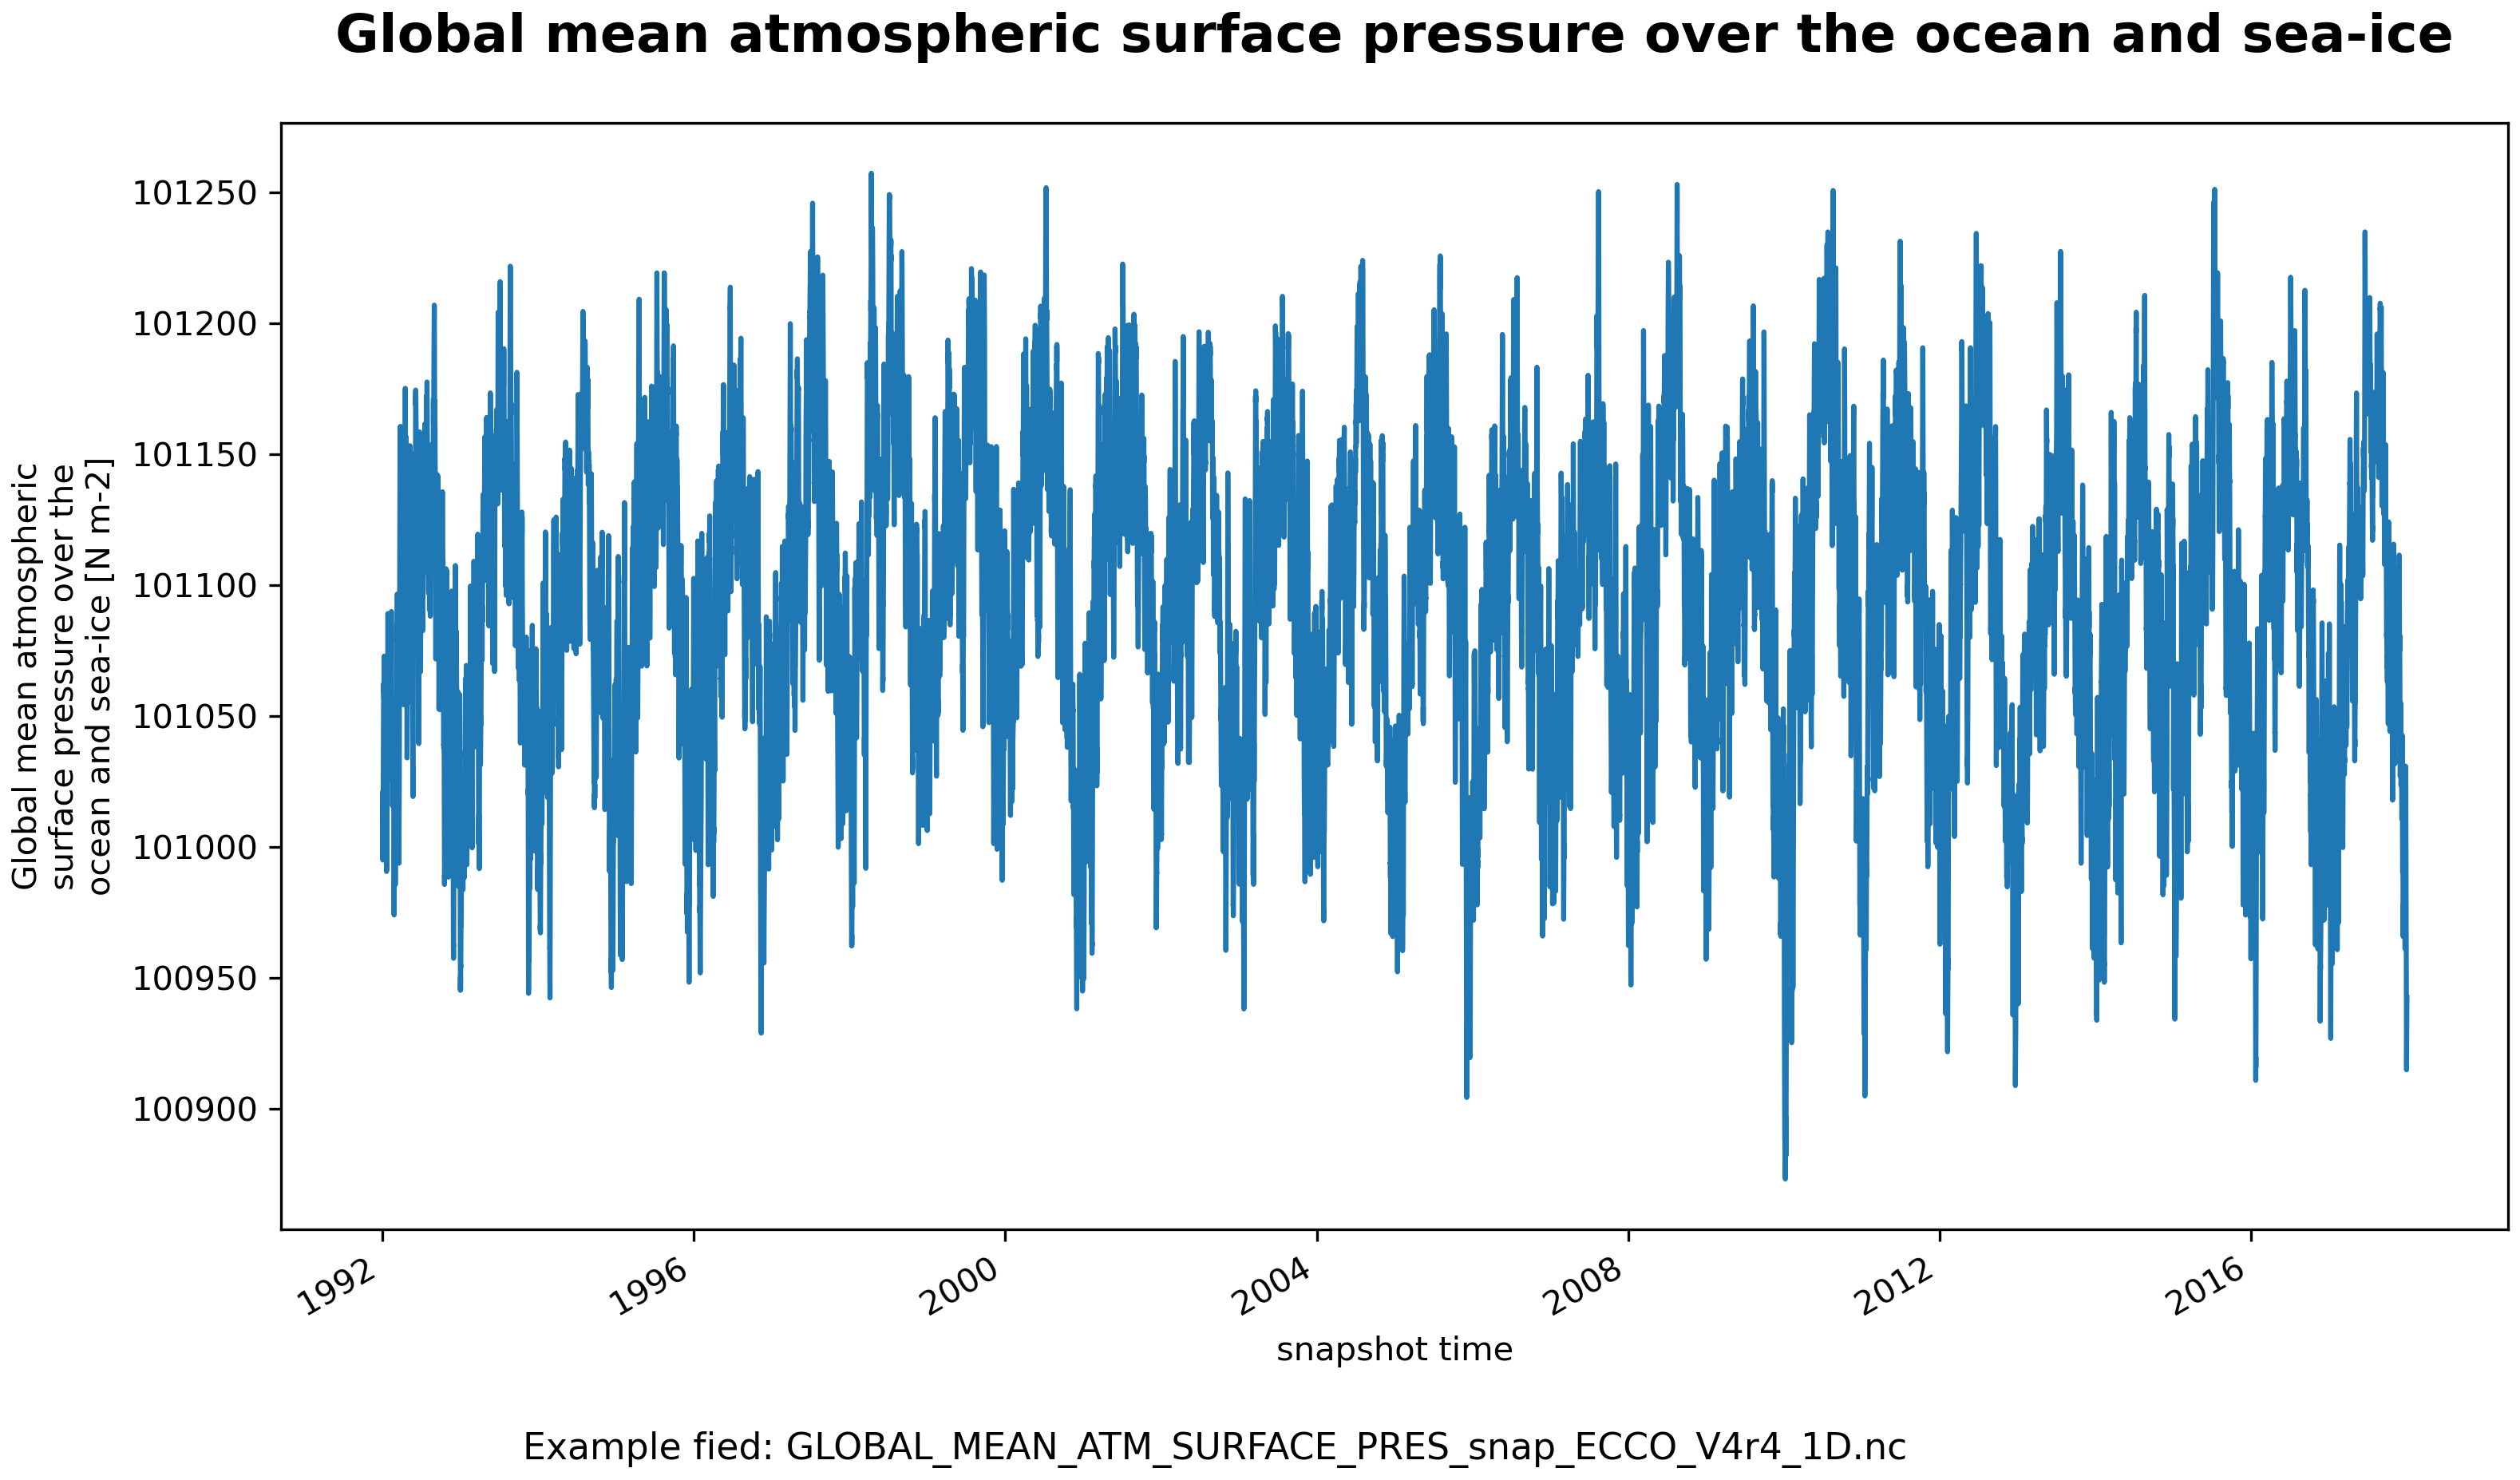
\includegraphics[scale=0.55]{../images/plots/oneD_plots/Global_Mean_Atmospheric_Pressure/Pa_global.png}
\caption{Dataset: GLOBAL\_MEAN\_ATM\_SURFACE\_PRES Variable: Pa\_global}
\label{tab:table-GLOBAL_MEAN_ATM_SURFACE_PRES_Pa_global-Plot}
\end{figure}
\pagebreak
\subsection{1D NetCDF GLOBAL\_MEAN\_SEA\_LEVEL}
\newp
\begin{longtable}{|p{0.1\textwidth}|p{0.5\textwidth}|}
\caption{Variables in the dataset GLOBAL\_MEAN\_SEA\_LEVEL}
\label{tab:table-GLOBAL_MEAN_SEA_LEVEL-fields} \\ 
\hline \endhead \hline \endfoot
\rowcolor{lightgray} \textbf{Dataset:} & \textbf{GLOBAL\_MEAN\_SEA\_LEVEL} \\ \hline
Field: &global\_mean\_barystatic\_sea\_level\_anomaly \\ \hline
Field: &global\_mean\_sea\_level\_anomaly \\ \hline
Field: &global\_mean\_sterodynamic\_sea\_level\_anomaly \\ \hline
\end{longtable}

\pagebreak
\subsubsection{1D Variable global\_mean\_barystatic\_sea\_level\_anomaly}
\begin{longtable}{|m{0.06\textwidth}|m{0.41\textwidth}|m{0.39\textwidth}|m{0.06\textwidth}|}
\caption{CDL description of GLOBAL\_MEAN\_SEA\_LEVEL's global\_mean\_barystatic\_sea\_level\_anomaly variable}
\label{tab:table-GLOBAL_MEAN_SEA_LEVEL_global_mean_barystatic_sea_level_anomaly} \\ 
\hline \endhead \hline \endfoot
\rowcolor{lightgray} \textbf{Storage Type} & \textbf{Variable Name} & \textbf{Description} & \textbf{Unit} \\ \hline
float32 & global\_mean\_barystatic\_sea\_level\_anomaly & Global mean of barystatic sea level anomaly & m \\ \hline
\rowcolor{lightgray}  \multicolumn{4}{|p{1.00\textwidth}|}{\textbf{CDL Description}} \\ \hline
\multicolumn{4}{|p{1.00\textwidth}|}{\makecell{\parbox{1\textwidth}{float32 global\_mean\_barystatic\_sea\_level\_anomaly(time)\\
\hspace*{0.5cm}global\_mean\_barystatic\_sea\_level\_anomaly: \_FillValue = 9.96921e+36\\
\hspace*{0.5cm}global\_mean\_barystatic\_sea\_level\_anomaly: coverage\_content\_type = modelResult\\
\hspace*{0.5cm}global\_mean\_barystatic\_sea\_level\_anomaly: long\_name = Global mean of barystatic sea level anomaly\\
\hspace*{0.5cm}global\_mean\_barystatic\_sea\_level\_anomaly: standard\_name = \\
\hspace*{0.5cm}global\_mean\_barystatic\_sea\_level\_anomaly: units = m\\
\hspace*{0.5cm}global\_mean\_barystatic\_sea\_level\_anomaly: valid\_min = : 0.045110904\\
\hspace*{0.5cm}global\_mean\_barystatic\_sea\_level\_anomaly: valid\_max = 0.043493364\\
\hspace*{0.5cm}global\_mean\_barystatic\_sea\_level\_anomaly: coordinates = time}}} \\ \hline
\rowcolor{lightgray} \multicolumn{4}{|p{1.00\textwidth}|}{\textbf{Comments}} \\ \hline
\multicolumn{4}{|p{1\textwidth}|}{Global mean barystatic sea level anomaly due to changes in total ocean mass. Note: ECCOv4 uses a volume-conserving Boussinesq formulation of the MITgcm with a free-surface boundary condition with real freshwater flux forcing. Changes in ocean mass due to evaporation, precipitation, runoff, and sea-ice growth/melt are reflected in model sea level. However, as a consequence of the Boussinsq formulation, changes to seawater density due to net buoyancy fluxes (e.g., global mean surface heating/cooling) do not change model sea level anomaly (ETAN) via seawater expansion/contraction. Changes in global ocean density therefore induce a spurious change in model ocean bottom pressure (PHIBOT) via 'virtual mass fluxes'. The 'Greatbatch correction' is a time varying, globally-uniform correction to account for changes in global mean density in Boussinesq models. This correction is used to calculate dynamic sea surface height (SSH) and ocean bottom pressure (OBP). Importantly, there is no dynamical significance to the Greatbatch correction but it is required to account for steric changes in global sea level. See Greatbatch, 1994. J. of Geophys. Res. Oceans, doi.org/10.1029/94JC00847} \\ \hline
\end{longtable}

\begin{figure}[H]
\centering
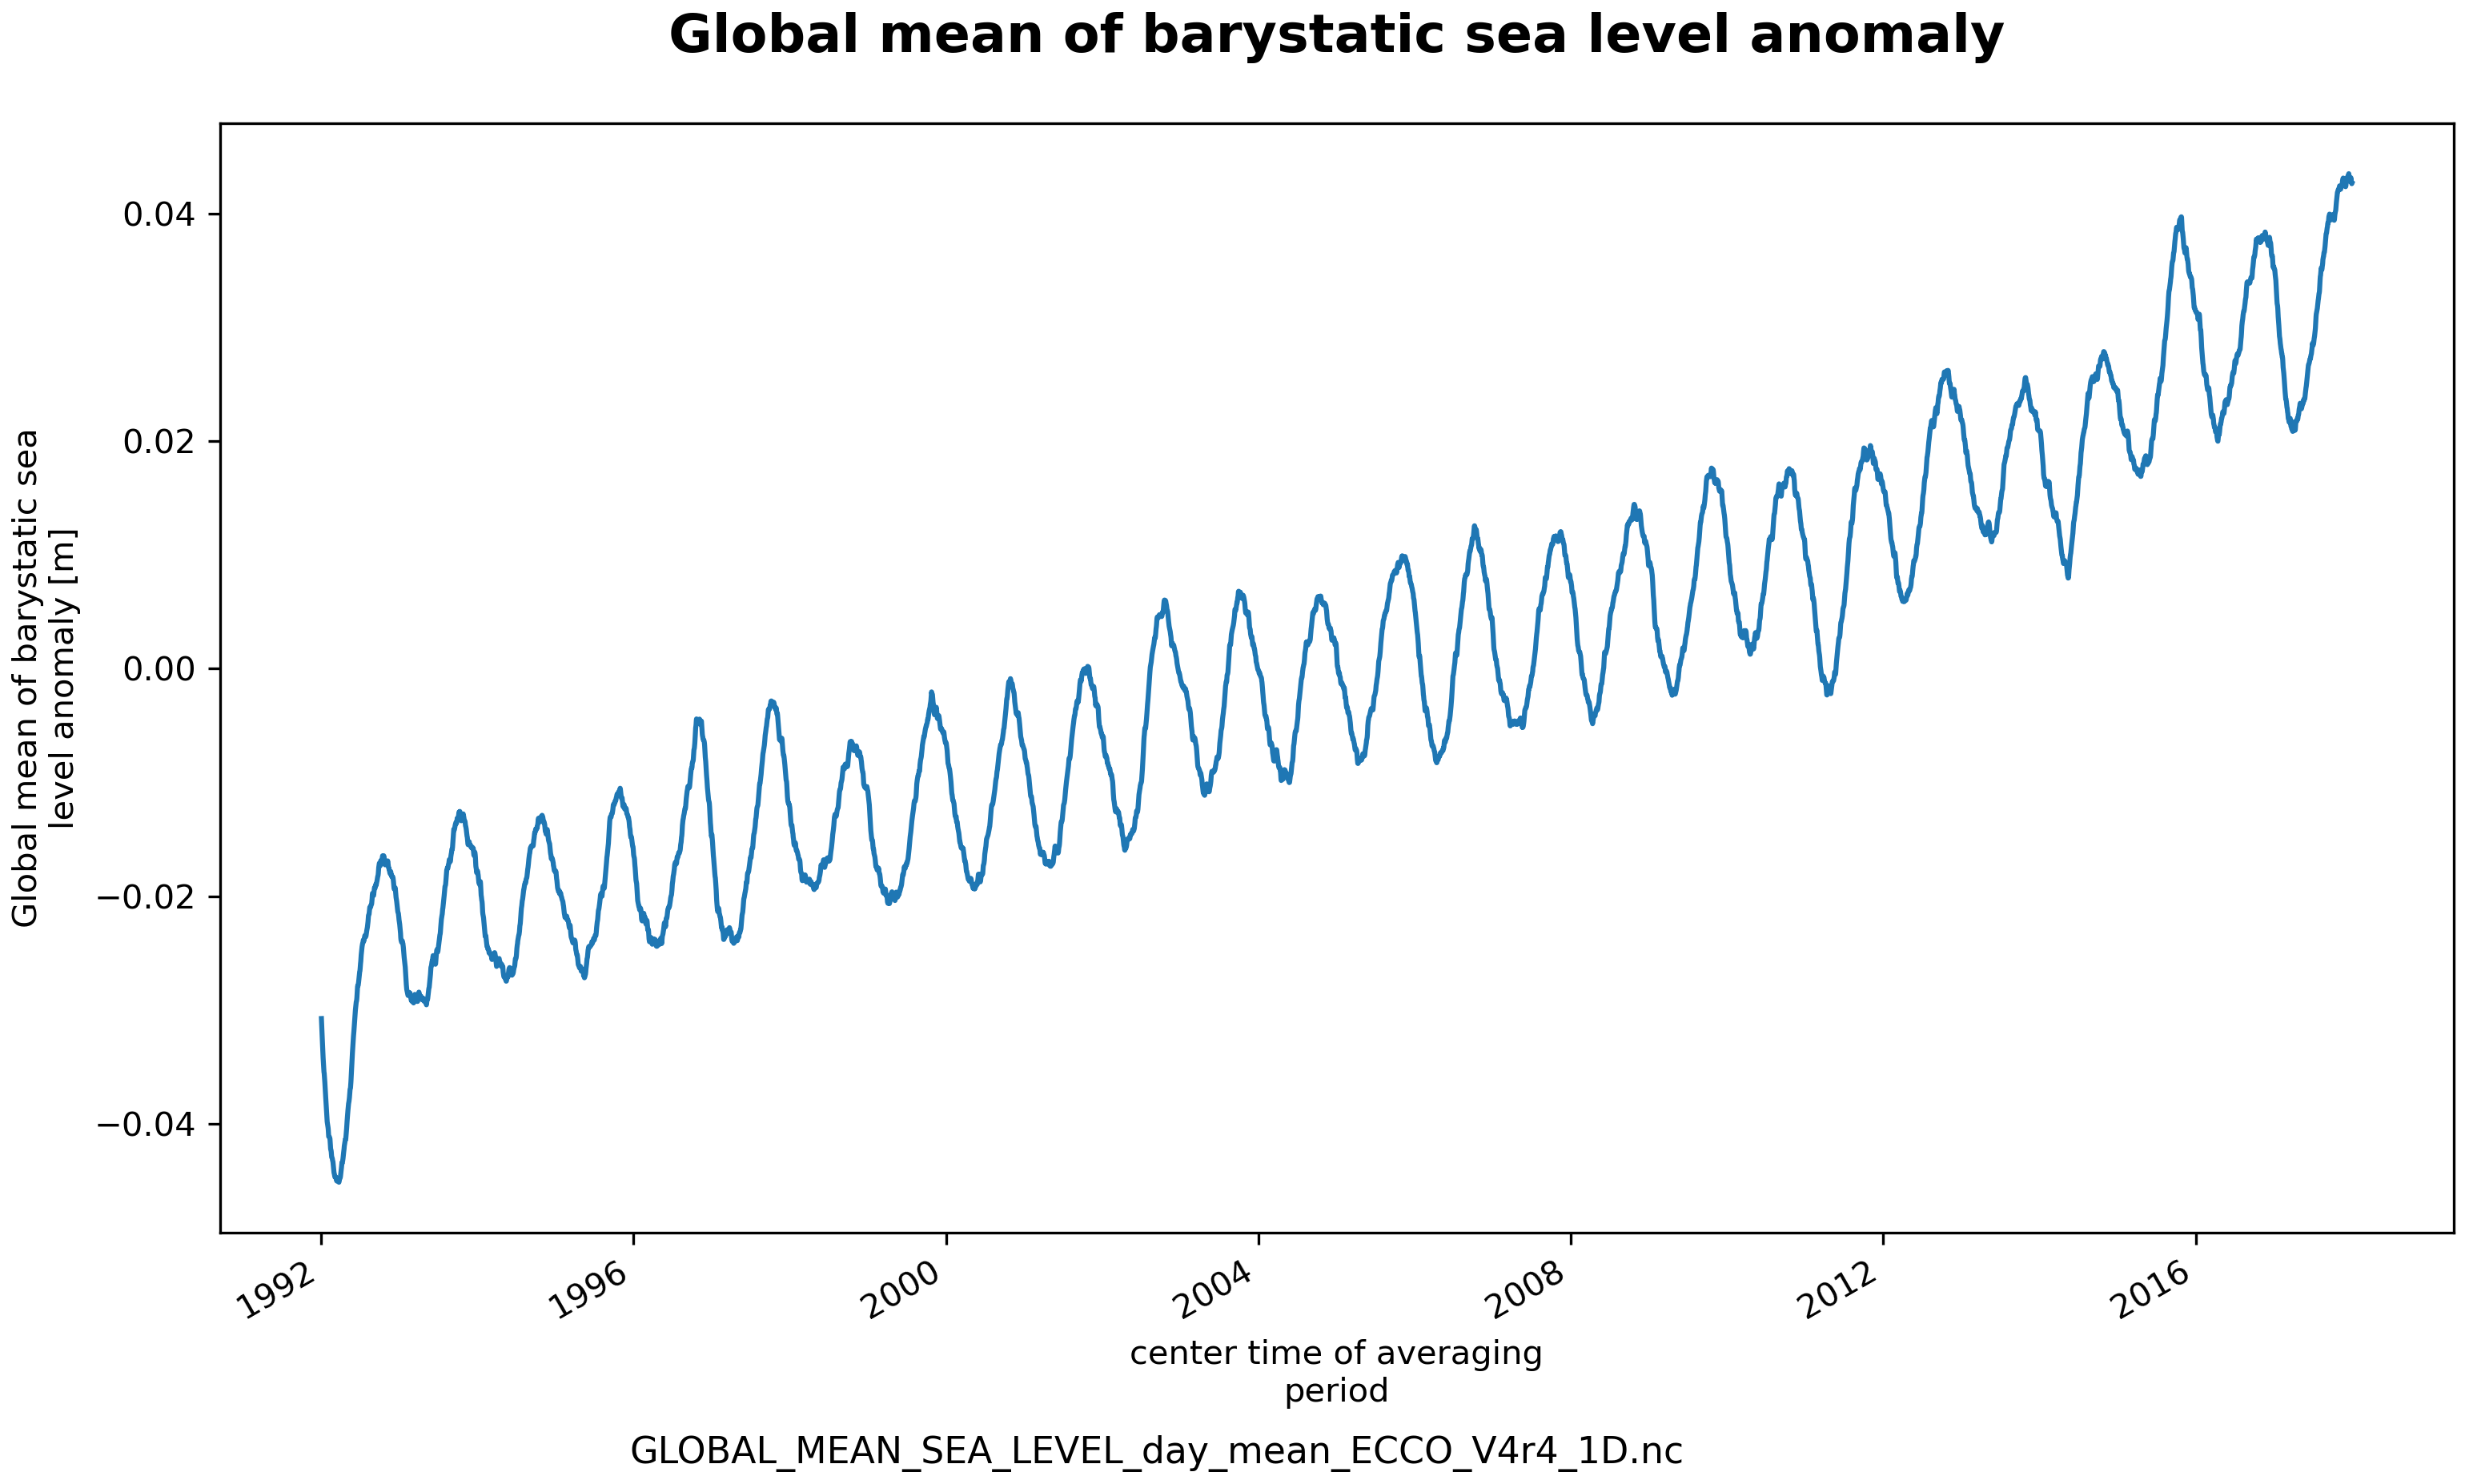
\includegraphics[scale=0.55]{../images/plots/oneD_plots/Global_Mean_Sea_Level/global_mean_barystatic_sea_level_anomaly.png}
\caption{Dataset: GLOBAL\_MEAN\_SEA\_LEVEL Variable: global\_mean\_barystatic\_sea\_level\_anomaly}
\label{tab:table-GLOBAL_MEAN_SEA_LEVEL_global_mean_barystatic_sea_level_anomaly-Plot}
\end{figure}
\pagebreak
\subsubsection{1D Variable global\_mean\_sea\_level\_anomaly}
\begin{longtable}{|m{0.06\textwidth}|m{0.41\textwidth}|m{0.39\textwidth}|m{0.06\textwidth}|}
\caption{CDL description of GLOBAL\_MEAN\_SEA\_LEVEL's global\_mean\_sea\_level\_anomaly variable}
\label{tab:table-GLOBAL_MEAN_SEA_LEVEL_global_mean_sea_level_anomaly} \\ 
\hline \endhead \hline \endfoot
\rowcolor{lightgray} \textbf{Storage Type} & \textbf{Variable Name} & \textbf{Description} & \textbf{Unit} \\ \hline
float32 & global\_mean\_sea\_level\_anomaly & Global mean of dynamic SSH & m \\ \hline
\rowcolor{lightgray}  \multicolumn{4}{|p{1.00\textwidth}|}{\textbf{CDL Description}} \\ \hline
\multicolumn{4}{|p{1.00\textwidth}|}{\makecell{\parbox{1\textwidth}{float32 global\_mean\_sea\_level\_anomaly(time)\\
\hspace*{0.5cm}global\_mean\_sea\_level\_anomaly: \_FillValue = 9.96921e+36\\
\hspace*{0.5cm}global\_mean\_sea\_level\_anomaly: coverage\_content\_type = modelResult\\
\hspace*{0.5cm}global\_mean\_sea\_level\_anomaly: long\_name = Global mean of dynamic SSH\\
\hspace*{0.5cm}global\_mean\_sea\_level\_anomaly: standard\_name = \\
\hspace*{0.5cm}global\_mean\_sea\_level\_anomaly: units = m\\
\hspace*{0.5cm}global\_mean\_sea\_level\_anomaly: valid\_min = : 0.055836163\\
\hspace*{0.5cm}global\_mean\_sea\_level\_anomaly: valid\_max = 0.05520557\\
\hspace*{0.5cm}global\_mean\_sea\_level\_anomaly: coordinates = time}}} \\ \hline
\rowcolor{lightgray} \multicolumn{4}{|p{1.00\textwidth}|}{\textbf{Comments}} \\ \hline
\multicolumn{4}{|p{1\textwidth}|}{Global mean of dynamic sea level anomaly, equivalent to global mean sea level change. Note: ECCOv4 uses a volume-conserving Boussinesq formulation of the MITgcm with a free-surface boundary condition with real freshwater flux forcing. Changes in ocean mass due to evaporation, precipitation, runoff, and sea-ice growth/melt are reflected in model sea level. However, as a consequence of the Boussinsq formulation, changes to seawater density due to net buoyancy fluxes (e.g., global mean surface heating/cooling) do not change model sea level anomaly (ETAN) via seawater expansion/contraction. Changes in global ocean density therefore induce a spurious change in model ocean bottom pressure (PHIBOT) via 'virtual mass fluxes'. The 'Greatbatch correction' is a time varying, globally-uniform correction to account for changes in global mean density in Boussinesq models. This correction is used to calculate dynamic sea surface height (SSH) and ocean bottom pressure (OBP). Importantly, there is no dynamical significance to the Greatbatch correction but it is required to account for steric changes in global sea level. See Greatbatch, 1994. J. of Geophys. Res. Oceans, doi.org/10.1029/94JC00847} \\ \hline
\end{longtable}

\begin{figure}[H]
\centering
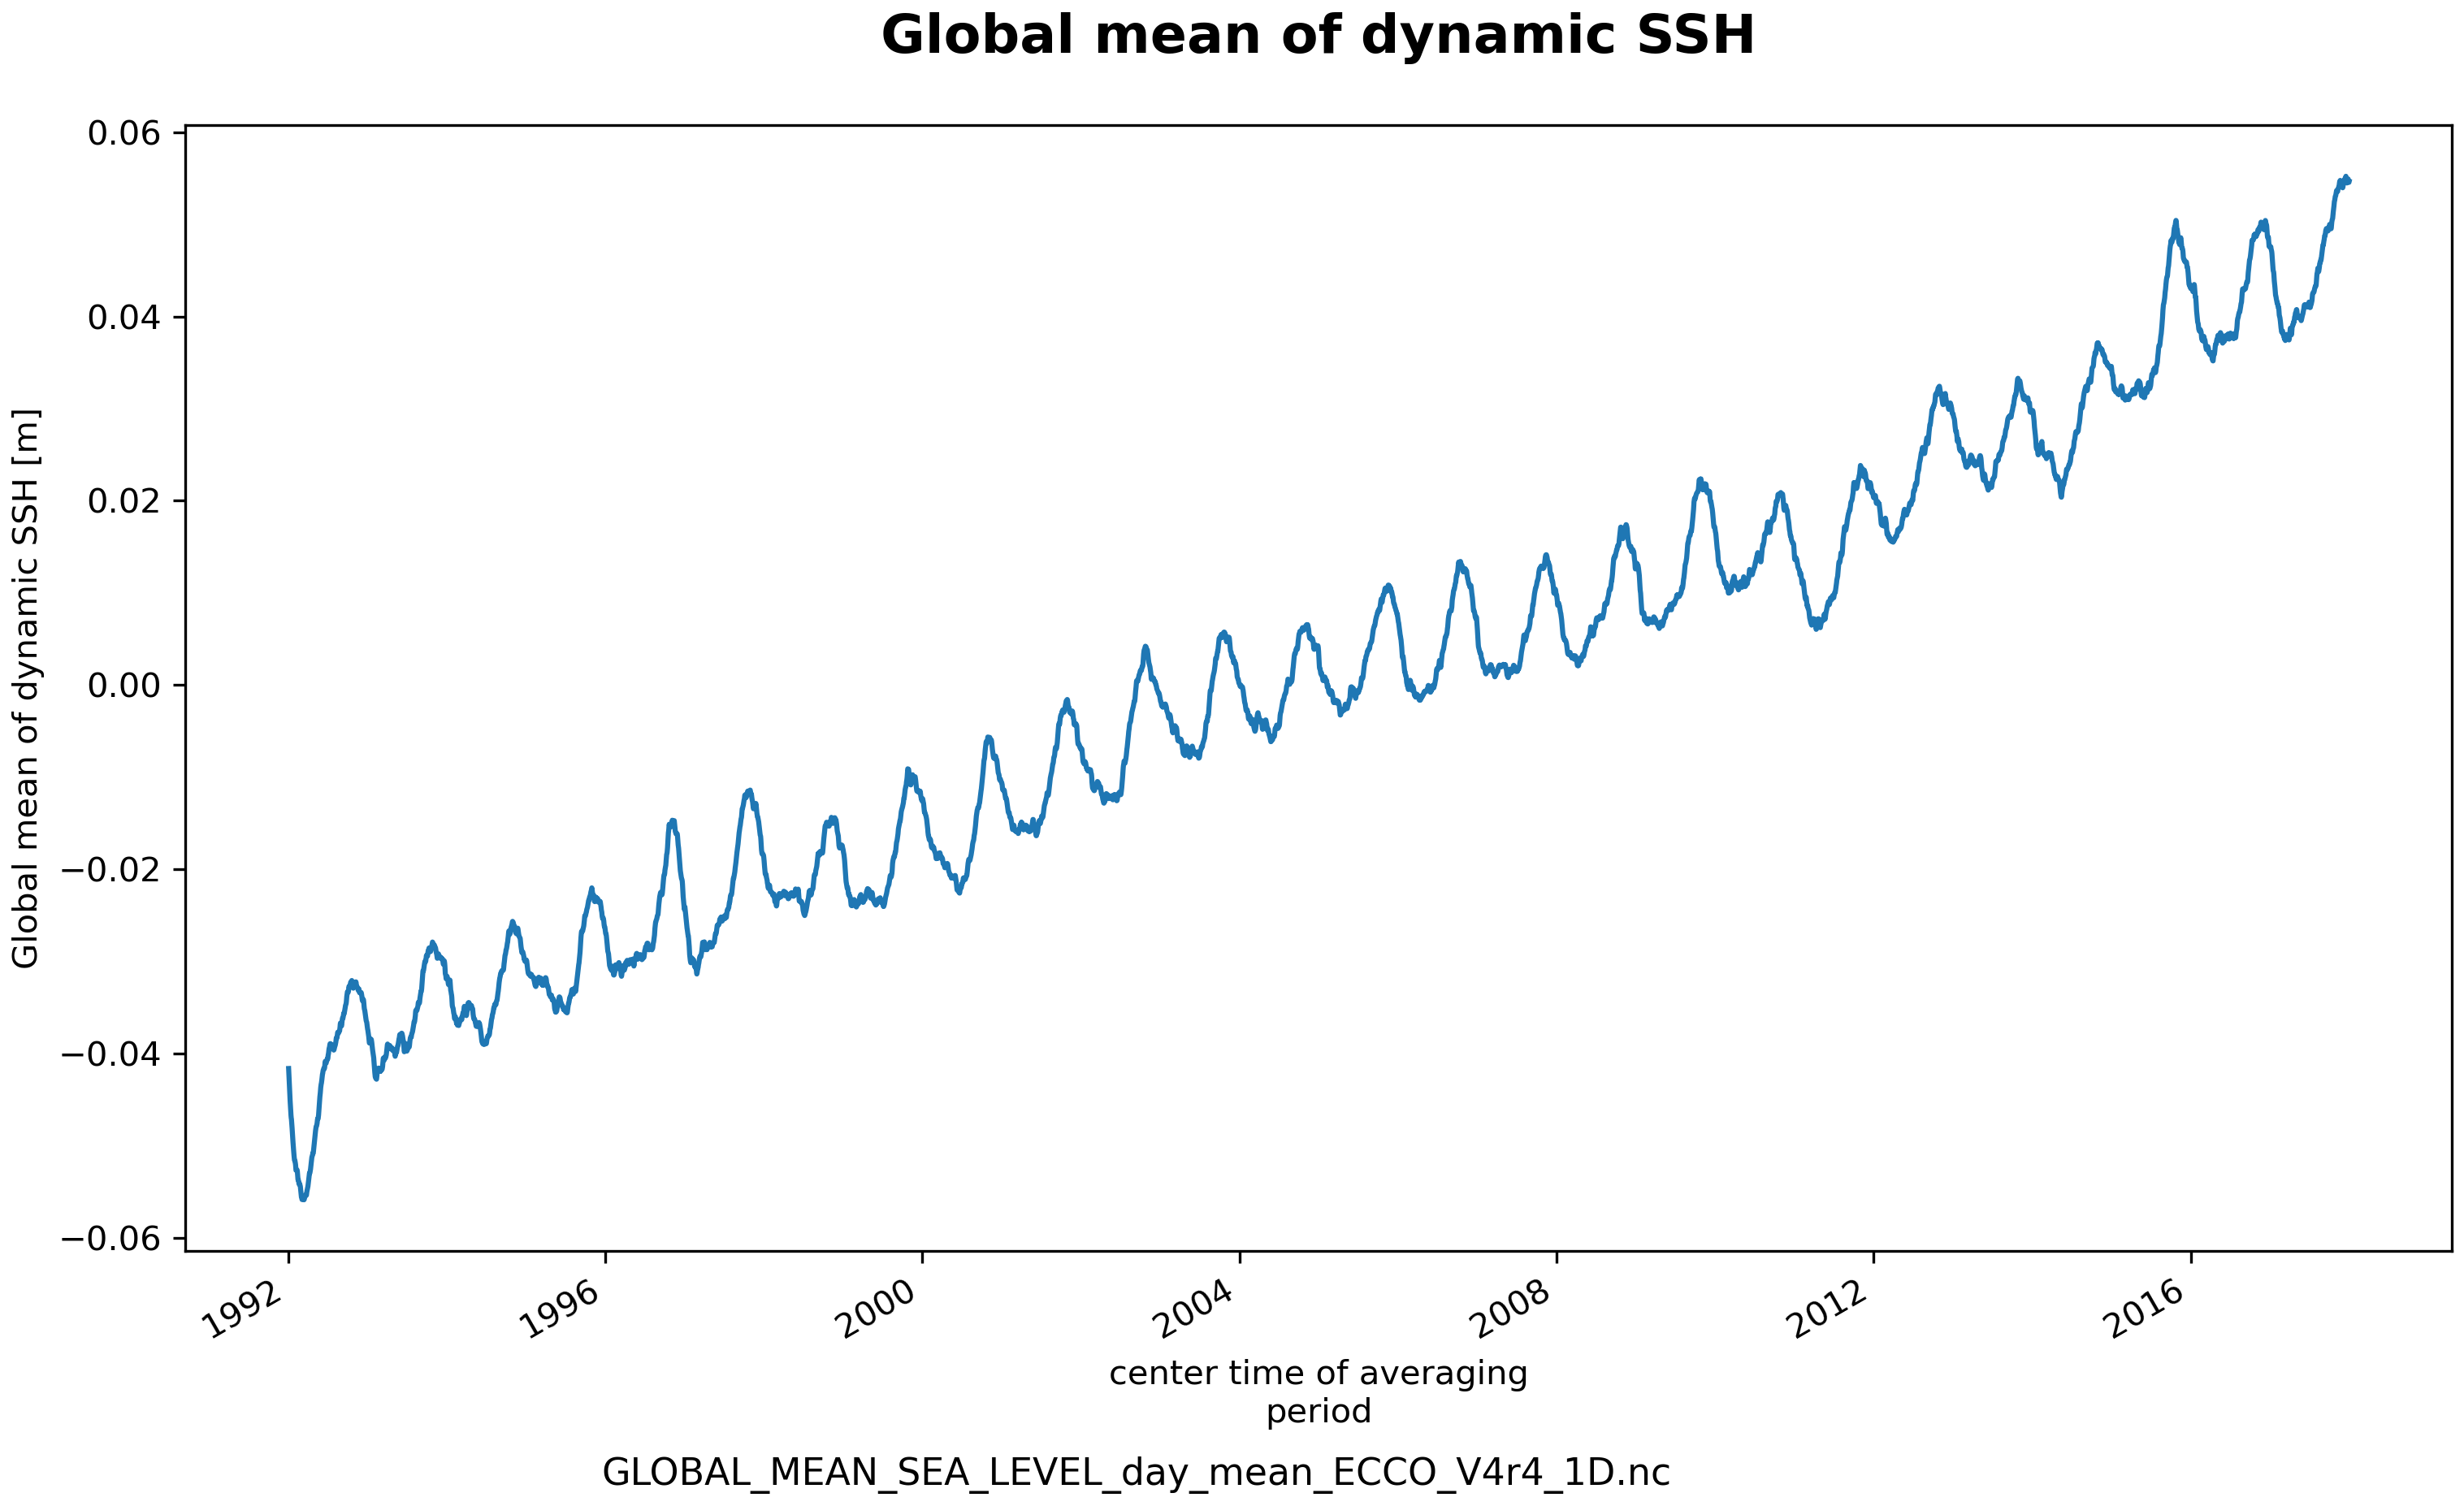
\includegraphics[scale=0.55]{../images/plots/oneD_plots/Global_Mean_Sea_Level/global_mean_sea_level_anomaly.png}
\caption{Dataset: GLOBAL\_MEAN\_SEA\_LEVEL Variable: global\_mean\_sea\_level\_anomaly}
\label{tab:table-GLOBAL_MEAN_SEA_LEVEL_global_mean_sea_level_anomaly-Plot}
\end{figure}
\pagebreak
\subsubsection{1D Variable global\_mean\_sterodynamic\_sea\_level\_anomaly}
\begin{longtable}{|m{0.06\textwidth}|m{0.41\textwidth}|m{0.39\textwidth}|m{0.06\textwidth}|}
\caption{CDL description of GLOBAL\_MEAN\_SEA\_LEVEL's global\_mean\_sterodynamic\_sea\_level\_anomaly variable}
\label{tab:table-GLOBAL_MEAN_SEA_LEVEL_global_mean_sterodynamic_sea_level_anomaly} \\ 
\hline \endhead \hline \endfoot
\rowcolor{lightgray} \textbf{Storage Type} & \textbf{Variable Name} & \textbf{Description} & \textbf{Unit} \\ \hline
float64 & global\_mean\_sterodynamic\_sea\_level\_anomaly & Global mean of sterodynamic sea level anomaly & m \\ \hline
\rowcolor{lightgray}  \multicolumn{4}{|p{1.00\textwidth}|}{\textbf{CDL Description}} \\ \hline
\multicolumn{4}{|p{1.00\textwidth}|}{\makecell{\parbox{1\textwidth}{float64 global\_mean\_sterodynamic\_sea\_level\_anomaly(time)\\
\hspace*{0.5cm}global\_mean\_sterodynamic\_sea\_level\_anomaly: \_FillValue = 9.969209968386869e+36\\
\hspace*{0.5cm}global\_mean\_sterodynamic\_sea\_level\_anomaly: coverage\_content\_type = modelResult\\
\hspace*{0.5cm}global\_mean\_sterodynamic\_sea\_level\_anomaly: long\_name = Global mean of sterodynamic sea level anomaly\\
\hspace*{0.5cm}global\_mean\_sterodynamic\_sea\_level\_anomaly: standard\_name = \\
\hspace*{0.5cm}global\_mean\_sterodynamic\_sea\_level\_anomaly: units = m\\
\hspace*{0.5cm}global\_mean\_sterodynamic\_sea\_level\_anomaly: valid\_min = : 0.017658796143049296\\
\hspace*{0.5cm}global\_mean\_sterodynamic\_sea\_level\_anomaly: valid\_max = 0.017642477223663407\\
\hspace*{0.5cm}global\_mean\_sterodynamic\_sea\_level\_anomaly: coordinates = time}}} \\ \hline
\rowcolor{lightgray} \multicolumn{4}{|p{1.00\textwidth}|}{\textbf{Comments}} \\ \hline
\multicolumn{4}{|p{1\textwidth}|}{Steric sea level anomaly associated with seawater expansion/contraction due to density changes. Note: ECCOv4 uses a volume-conserving Boussinesq formulation of the MITgcm with a free-surface boundary condition with real freshwater flux forcing. Changes in ocean mass due to evaporation, precipitation, runoff, and sea-ice growth/melt are reflected in model sea level. However, as a consequence of the Boussinsq formulation, changes to seawater density due to net buoyancy fluxes (e.g., global mean surface heating/cooling) do not change model sea level anomaly (ETAN) via seawater expansion/contraction. Changes in global ocean density therefore induce a spurious change in model ocean bottom pressure (PHIBOT) via 'virtual mass fluxes'. The 'Greatbatch correction' is a time varying, globally-uniform correction to account for changes in global mean density in Boussinesq models. This correction is used to calculate dynamic sea surface height (SSH) and ocean bottom pressure (OBP). Importantly, there is no dynamical significance to the Greatbatch correction but it is required to account for steric changes in global sea level. See Greatbatch, 1994. J. of Geophys. Res. Oceans, doi.org/10.1029/94JC00847} \\ \hline
\end{longtable}

\begin{figure}[H]
\centering
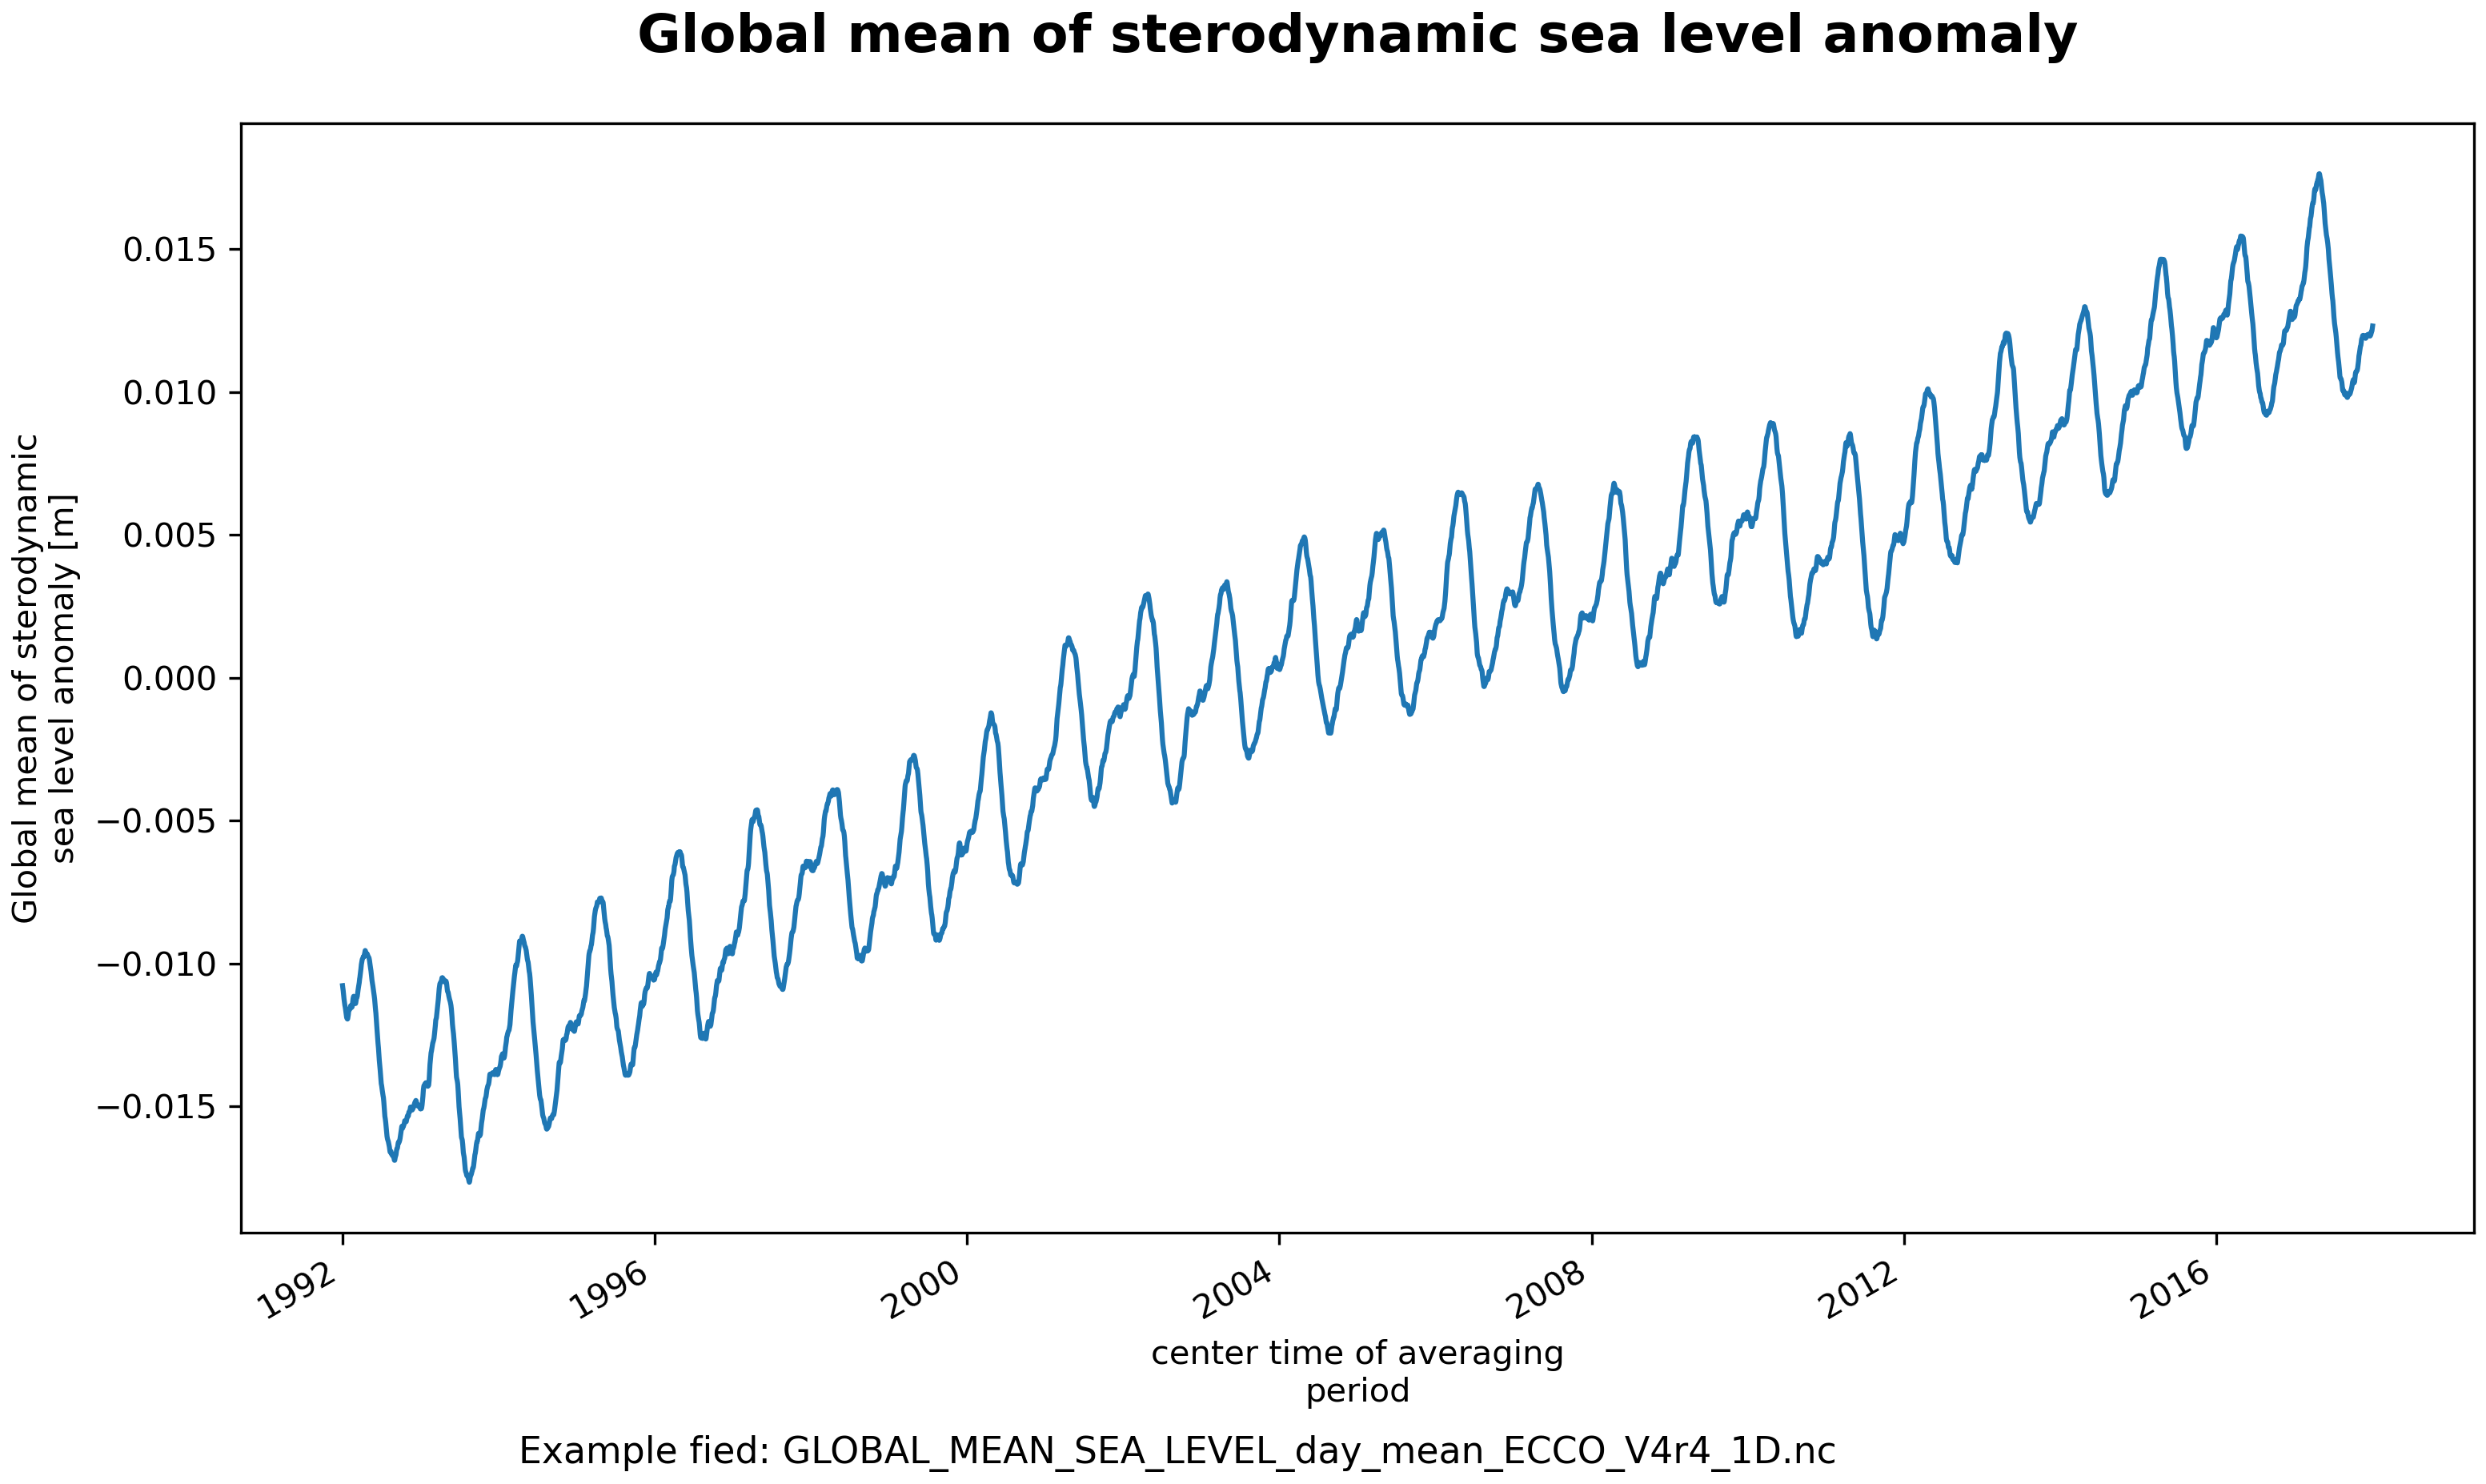
\includegraphics[scale=0.55]{../images/plots/oneD_plots/Global_Mean_Sea_Level/global_mean_sterodynamic_sea_level_anomaly.png}
\caption{Dataset: GLOBAL\_MEAN\_SEA\_LEVEL Variable: global\_mean\_sterodynamic\_sea\_level\_anomaly}
\label{tab:table-GLOBAL_MEAN_SEA_LEVEL_global_mean_sterodynamic_sea_level_anomaly-Plot}
\end{figure}
\pagebreak
\subsection{1D NetCDF SBO\_CORE\_PRODUCTS}
\newp
\begin{longtable}{|p{0.1\textwidth}|p{0.5\textwidth}|}
\caption{Variables in the dataset SBO\_CORE\_PRODUCTS}
\label{tab:table-SBO_CORE_PRODUCTS-fields} \\ 
\hline \endhead \hline \endfoot
\rowcolor{lightgray} \textbf{Dataset:} & \textbf{SBO\_CORE\_PRODUCTS} \\ \hline
Field: &xoamc \\ \hline
Field: &yoamc \\ \hline
Field: &zoamc \\ \hline
Field: &xoamp \\ \hline
Field: &yoamp \\ \hline
Field: &zoamp \\ \hline
Field: &mass \\ \hline
Field: &xcom \\ \hline
Field: &ycom \\ \hline
Field: &zcom \\ \hline
Field: &sboarea \\ \hline
Field: &xoamc\_si \\ \hline
Field: &yoamc\_si \\ \hline
Field: &zoamc\_si \\ \hline
Field: &mass\_si \\ \hline
Field: &xoamp\_fw \\ \hline
Field: &yoamp\_fw \\ \hline
Field: &zoamp\_fw \\ \hline
Field: &mass\_fw \\ \hline
Field: &xcom\_fw \\ \hline
Field: &ycom\_fw \\ \hline
Field: &zcom\_fw \\ \hline
Field: &mass\_gc \\ \hline
Field: &xoamp\_dsl \\ \hline
Field: &yoamp\_dsl \\ \hline
Field: &zoamp\_dsl \\ \hline
\end{longtable}

\pagebreak
\subsubsection{1D Variable mass}
\begin{longtable}{|m{0.06\textwidth}|m{0.41\textwidth}|m{0.39\textwidth}|m{0.06\textwidth}|}
\caption{CDL description of SBO\_CORE\_PRODUCTS's mass variable}
\label{tab:table-SBO_CORE_PRODUCTS_mass} \\ 
\hline \endhead \hline \endfoot
\rowcolor{lightgray} \textbf{Storage Type} & \textbf{Variable Name} & \textbf{Description} & \textbf{Unit} \\ \hline
float64 & mass & ocean mass & kg \\ \hline
\rowcolor{lightgray}  \multicolumn{4}{|p{1.00\textwidth}|}{\textbf{CDL Description}} \\ \hline
\multicolumn{4}{|p{1.00\textwidth}|}{\makecell{\parbox{1\textwidth}{float64 mass(time)\\
\hspace*{0.5cm}mass: \_FillValue = 9.969209968386869e+36\\
\hspace*{0.5cm}mass: coverage\_content\_type = modelResult\\
\hspace*{0.5cm}mass: long\_name = ocean\hspace*{0.5cm} mass\\
\hspace*{0.5cm}mass: units = kg\\
\hspace*{0.5cm}mass: valid\_min = 1.3737507447512265e+21\\
\hspace*{0.5cm}mass: valid\_max = 1.3737832079900274e+21\\
\hspace*{0.5cm}mass: coordinates = time}}} \\ \hline
\rowcolor{lightgray} \multicolumn{4}{|p{1.00\textwidth}|}{\textbf{Comments}} \\ \hline
\multicolumn{4}{|p{1\textwidth}|}{N/A} \\ \hline
\end{longtable}

\begin{figure}[H]
\centering
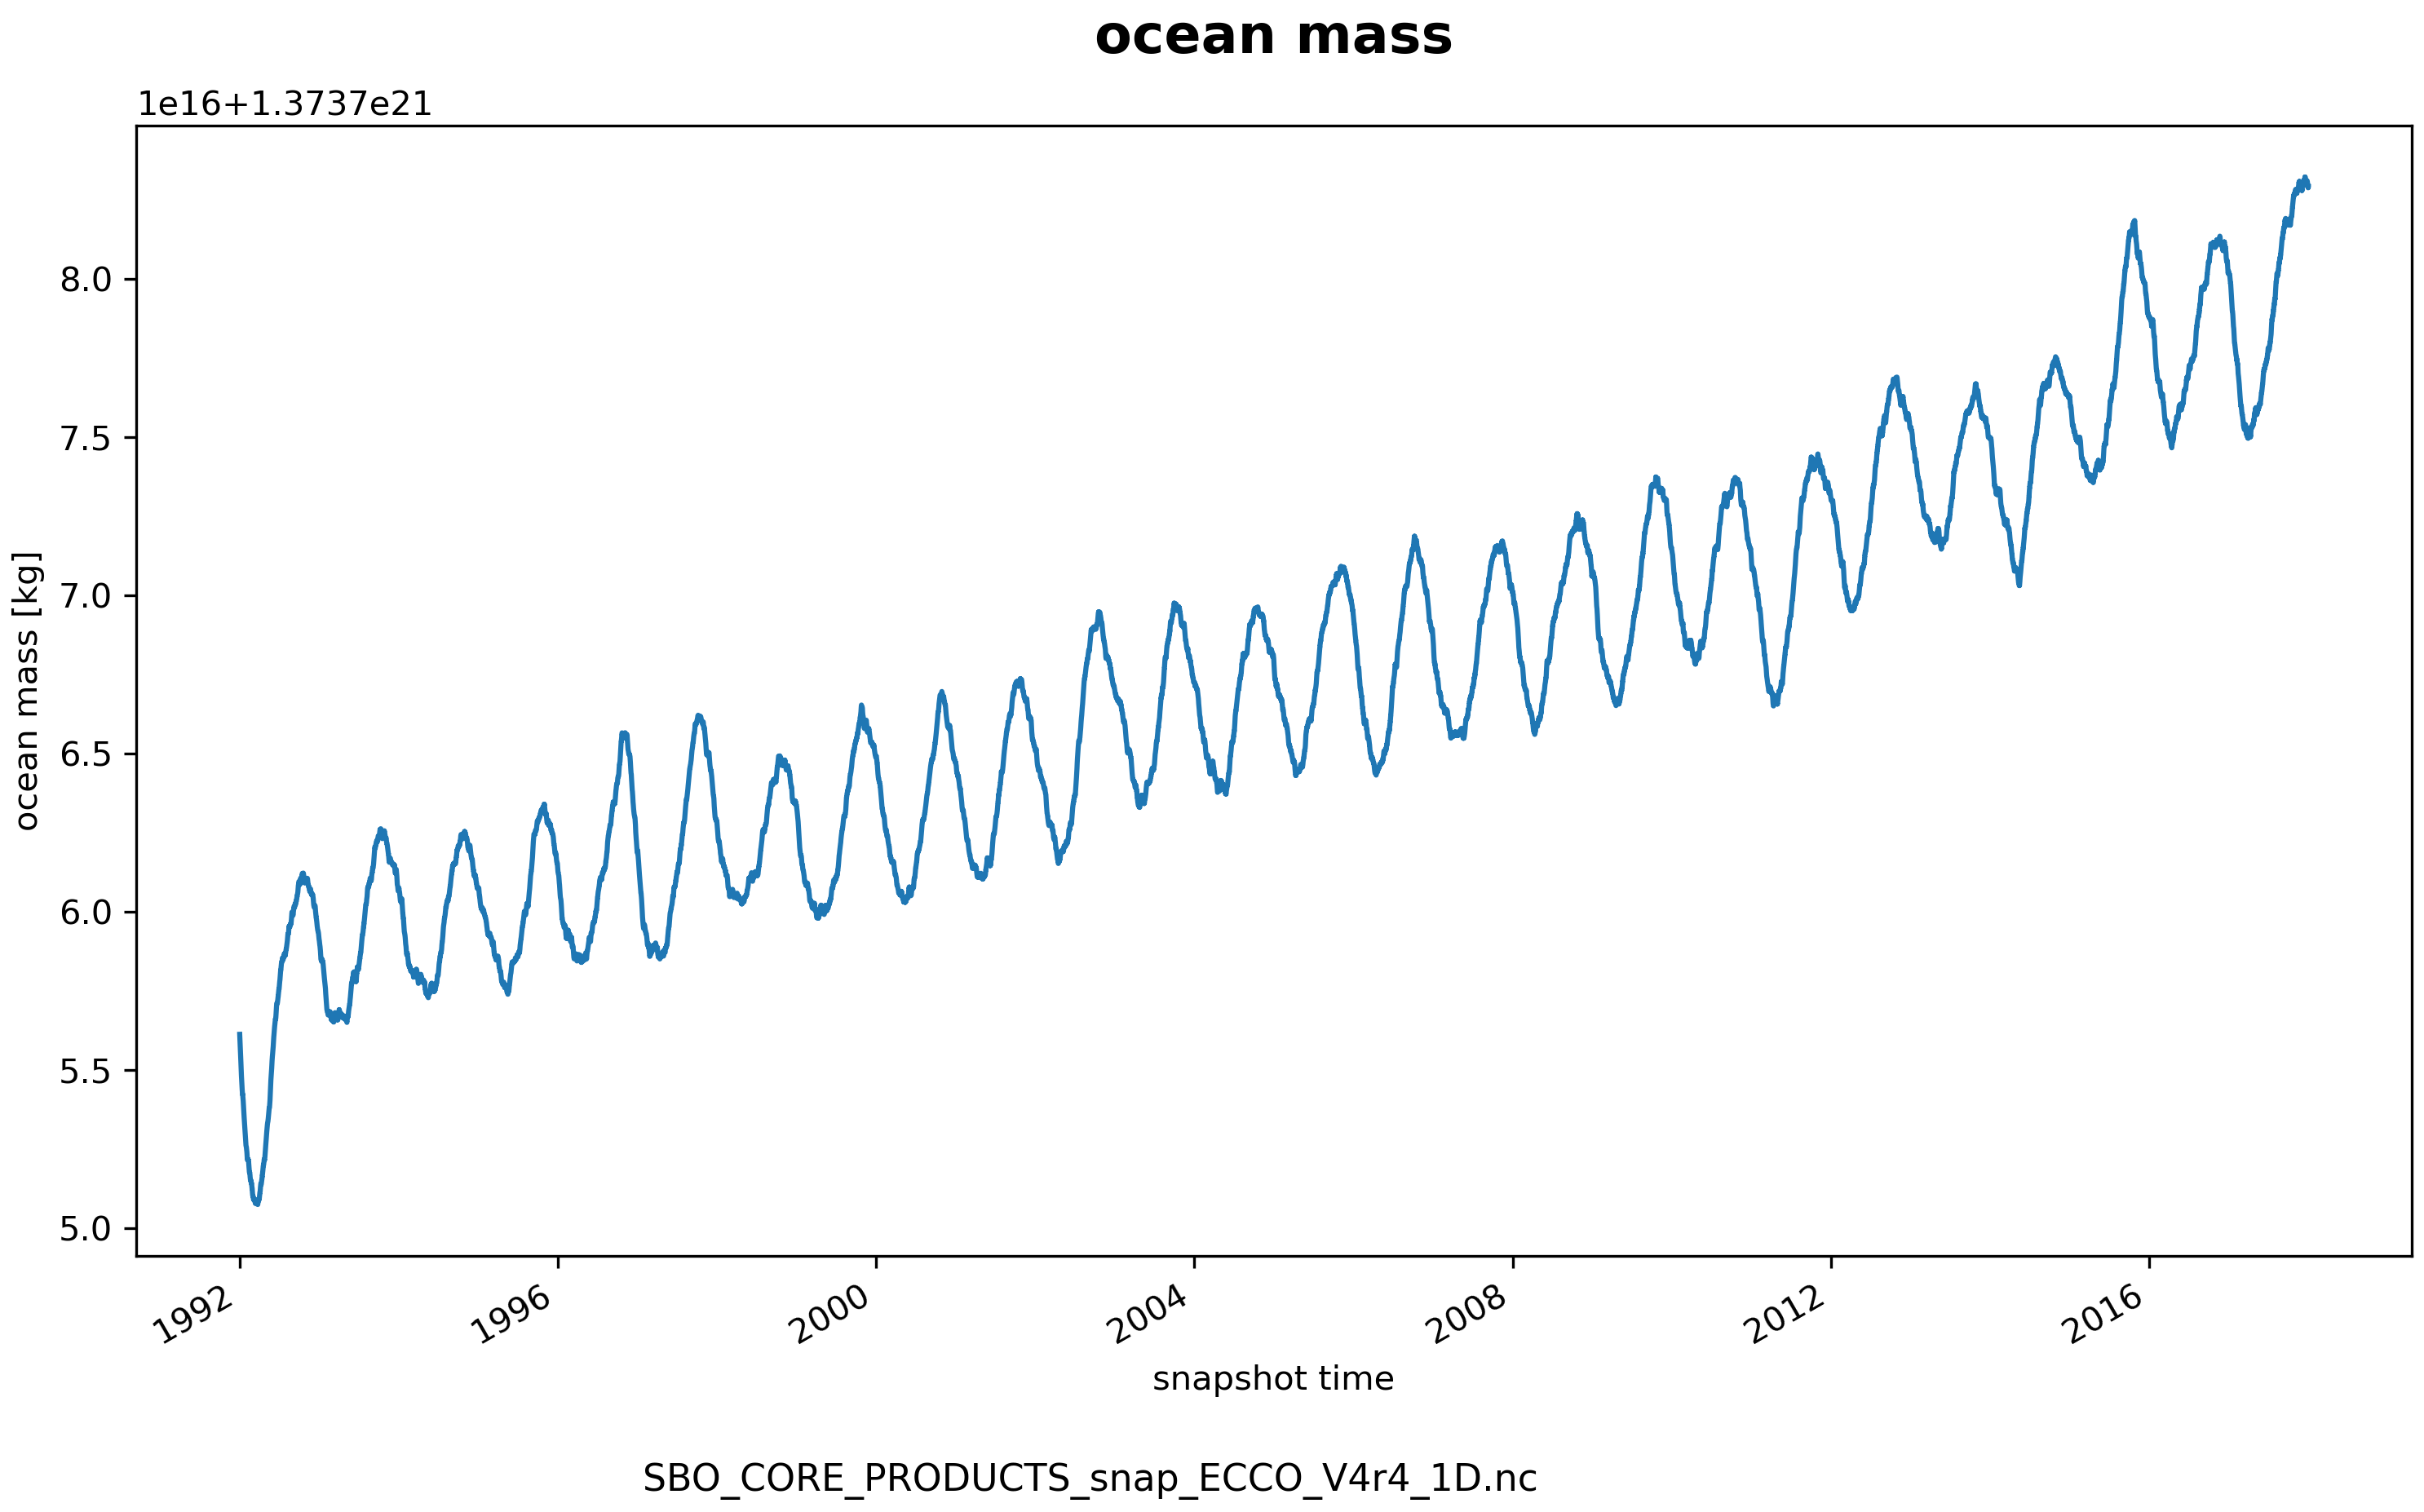
\includegraphics[scale=0.55]{../images/plots/oneD_plots/SBO_Core_Products/mass.png}
\caption{Dataset: SBO\_CORE\_PRODUCTS Variable: mass}
\label{tab:table-SBO_CORE_PRODUCTS_mass-Plot}
\end{figure}
\pagebreak
\subsubsection{1D Variable mass\_fw}
\begin{longtable}{|m{0.06\textwidth}|m{0.41\textwidth}|m{0.39\textwidth}|m{0.06\textwidth}|}
\caption{CDL description of SBO\_CORE\_PRODUCTS's mass\_fw variable}
\label{tab:table-SBO_CORE_PRODUCTS_mass_fw} \\ 
\hline \endhead \hline \endfoot
\rowcolor{lightgray} \textbf{Storage Type} & \textbf{Variable Name} & \textbf{Description} & \textbf{Unit} \\ \hline
float64 & mass\_fw & mass due to freshwater flux & kg \\ \hline
\rowcolor{lightgray}  \multicolumn{4}{|p{1.00\textwidth}|}{\textbf{CDL Description}} \\ \hline
\multicolumn{4}{|p{1.00\textwidth}|}{\makecell{\parbox{1\textwidth}{float64 mass\_fw(time)\\
\hspace*{0.5cm}mass\_fw: \_FillValue = 9.969209968386869e+36\\
\hspace*{0.5cm}mass\_fw: coverage\_content\_type = modelResult\\
\hspace*{0.5cm}mass\_fw: long\_name = mass due to freshwater flux\\
\hspace*{0.5cm}mass\_fw: units = kg\\
\hspace*{0.5cm}mass\_fw: valid\_min = 3.7929380693921944e+16\\
\hspace*{0.5cm}mass\_fw: valid\_max = 7.0392619494226936e+16\\
\hspace*{0.5cm}mass\_fw: coordinates = time}}} \\ \hline
\rowcolor{lightgray} \multicolumn{4}{|p{1.00\textwidth}|}{\textbf{Comments}} \\ \hline
\multicolumn{4}{|p{1\textwidth}|}{N/A} \\ \hline
\end{longtable}

\begin{figure}[H]
\centering
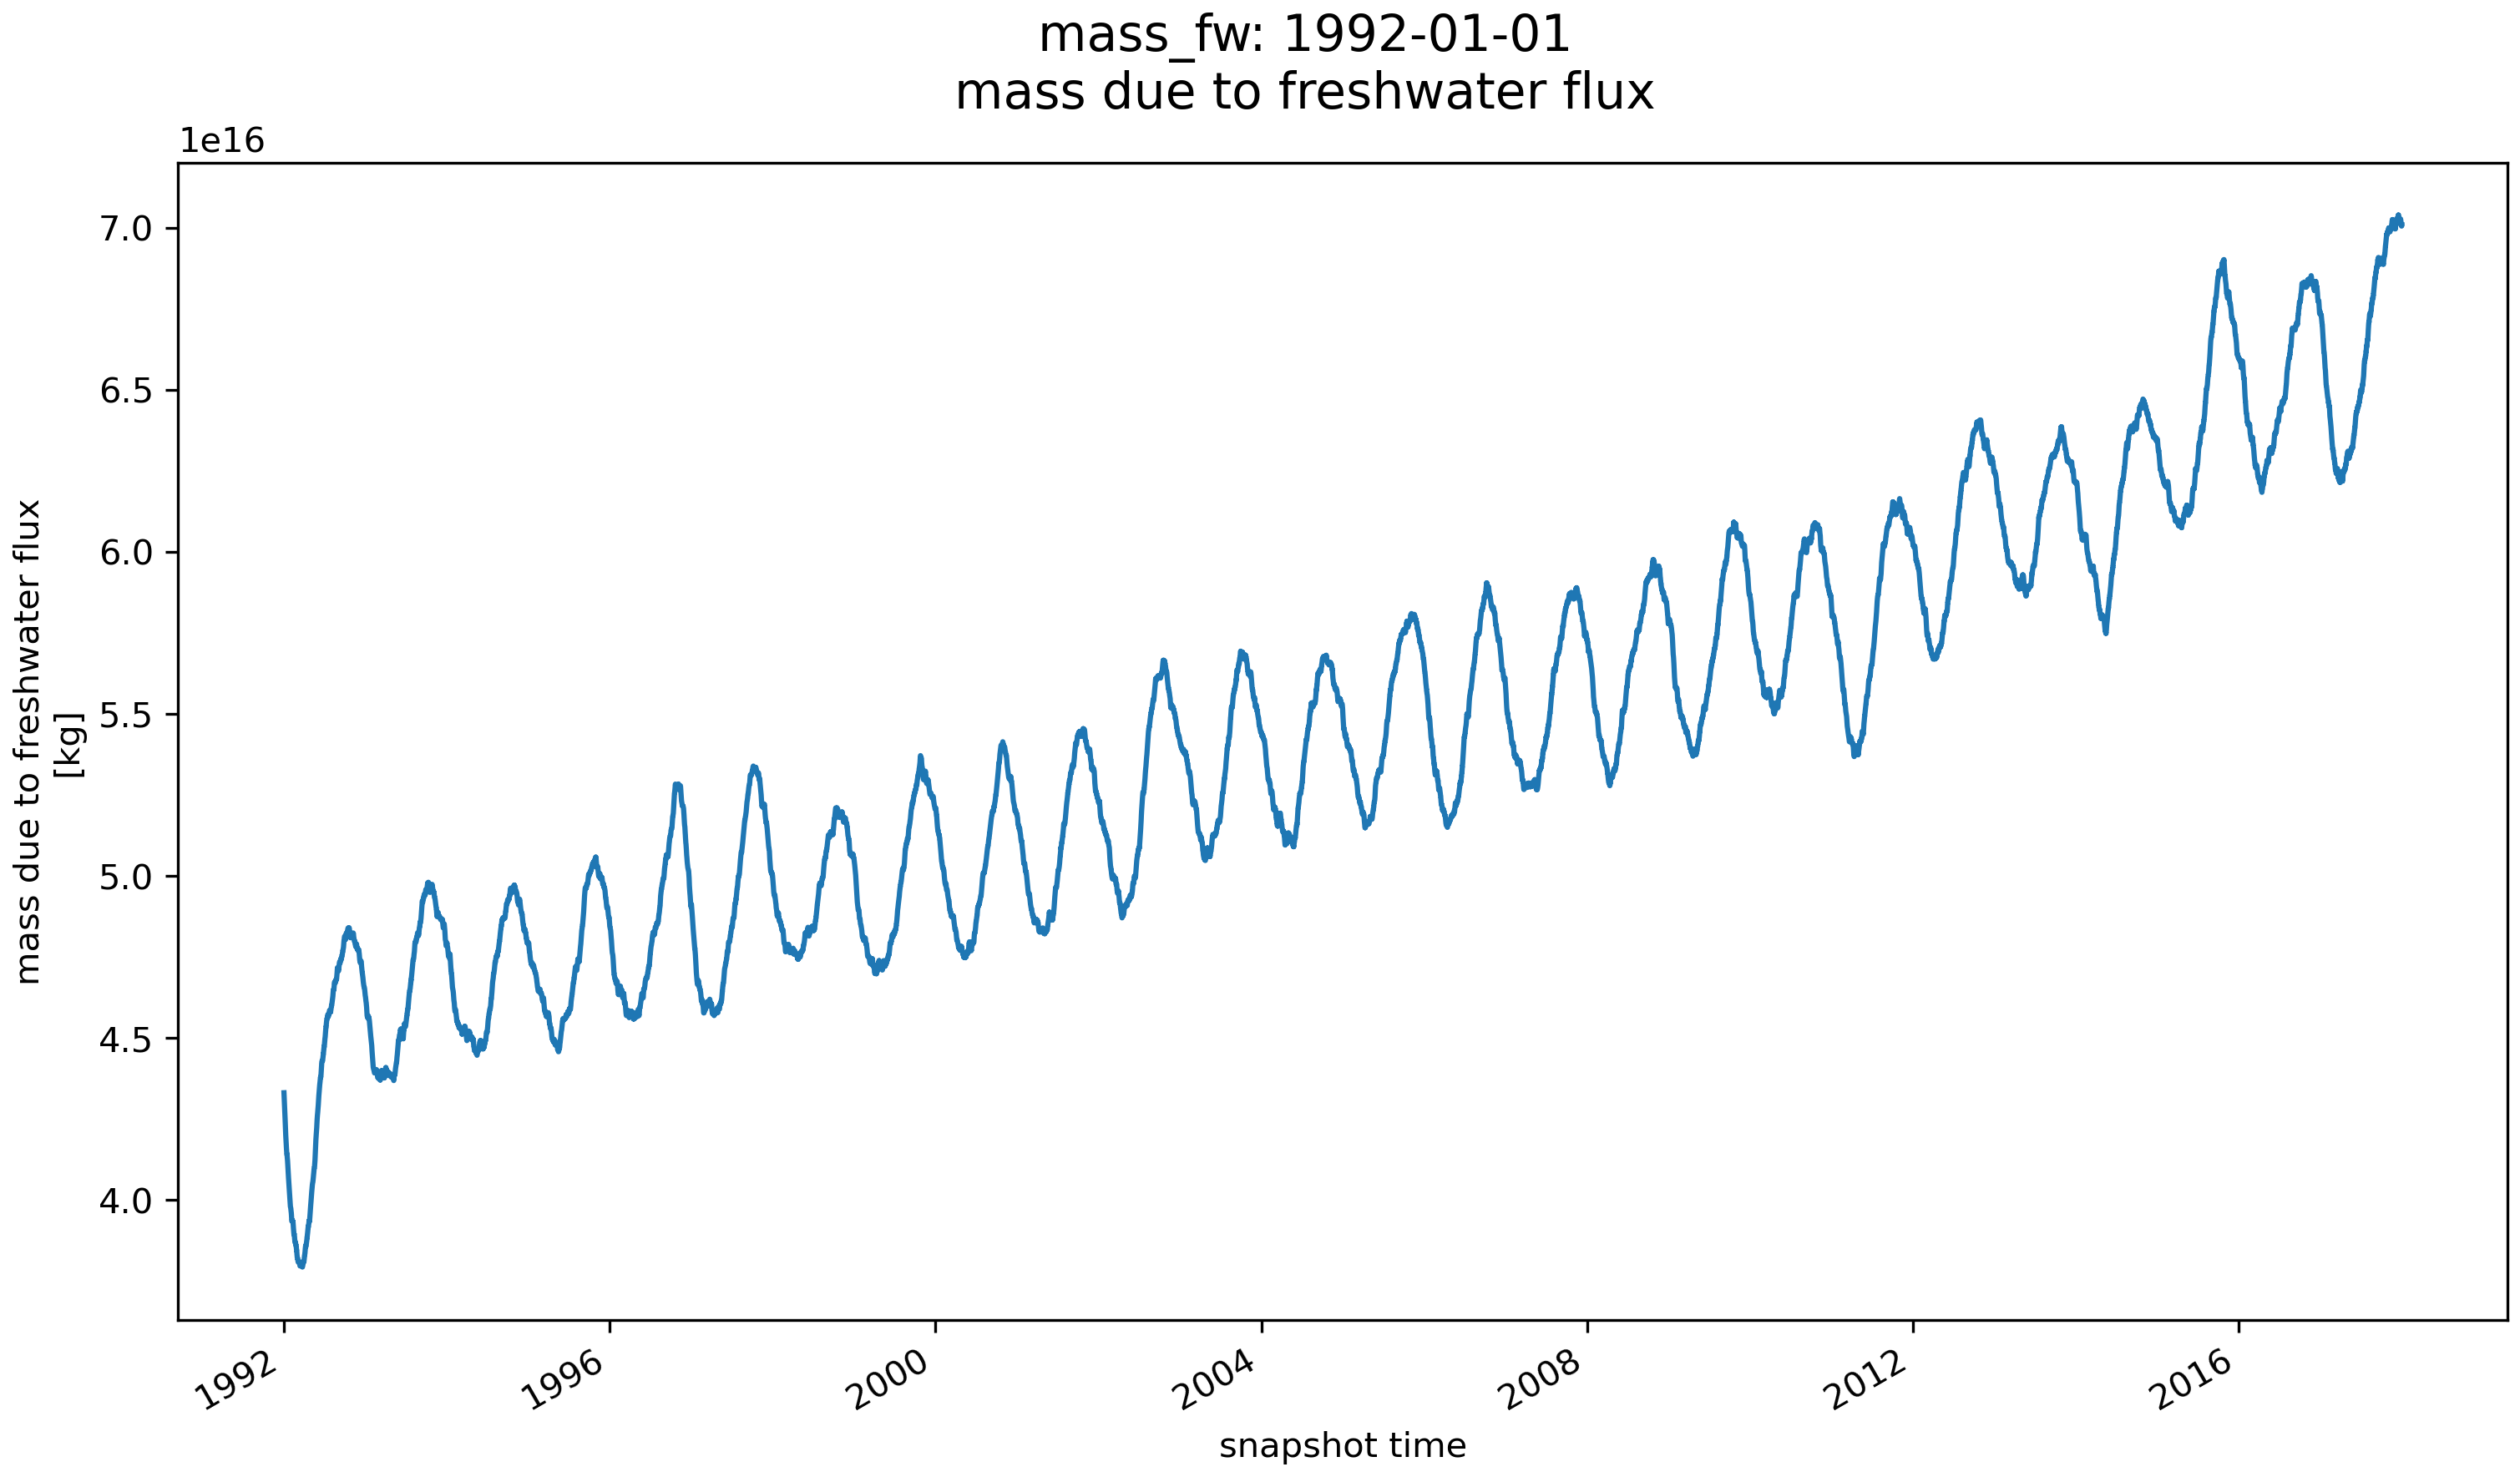
\includegraphics[scale=0.55]{../images/plots/oneD_plots/SBO_Core_Products/mass_fw.png}
\caption{Dataset: SBO\_CORE\_PRODUCTS Variable: mass\_fw}
\label{tab:table-SBO_CORE_PRODUCTS_mass_fw-Plot}
\end{figure}
\pagebreak
\subsubsection{1D Variable mass\_gc}
\begin{longtable}{|m{0.06\textwidth}|m{0.41\textwidth}|m{0.39\textwidth}|m{0.06\textwidth}|}
\caption{CDL description of SBO\_CORE\_PRODUCTS's mass\_gc variable}
\label{tab:table-SBO_CORE_PRODUCTS_mass_gc} \\ 
\hline \endhead \hline \endfoot
\rowcolor{lightgray} \textbf{Storage Type} & \textbf{Variable Name} & \textbf{Description} & \textbf{Unit} \\ \hline
float64 & mass\_gc & mass due to the Greatbatch correction & kg \\ \hline
\rowcolor{lightgray}  \multicolumn{4}{|p{1.00\textwidth}|}{\textbf{CDL Description}} \\ \hline
\multicolumn{4}{|p{1.00\textwidth}|}{\makecell{\parbox{1\textwidth}{float64 mass\_gc(time)\\
\hspace*{0.5cm}mass\_gc: \_FillValue = 9.969209968386869e+36\\
\hspace*{0.5cm}mass\_gc: coverage\_content\_type = modelResult\\
\hspace*{0.5cm}mass\_gc: long\_name = mass due to the Greatbatch correction\\
\hspace*{0.5cm}mass\_gc: units = kg\\
\hspace*{0.5cm}mass\_gc: valid\_min = : 1.140148294309558e+19\\
\hspace*{0.5cm}mass\_gc: valid\_max = : 1.1388436906537843e+19\\
\hspace*{0.5cm}mass\_gc: coordinates = time}}} \\ \hline
\rowcolor{lightgray} \multicolumn{4}{|p{1.00\textwidth}|}{\textbf{Comments}} \\ \hline
\multicolumn{4}{|p{1\textwidth}|}{N/A} \\ \hline
\end{longtable}

\begin{figure}[H]
\centering
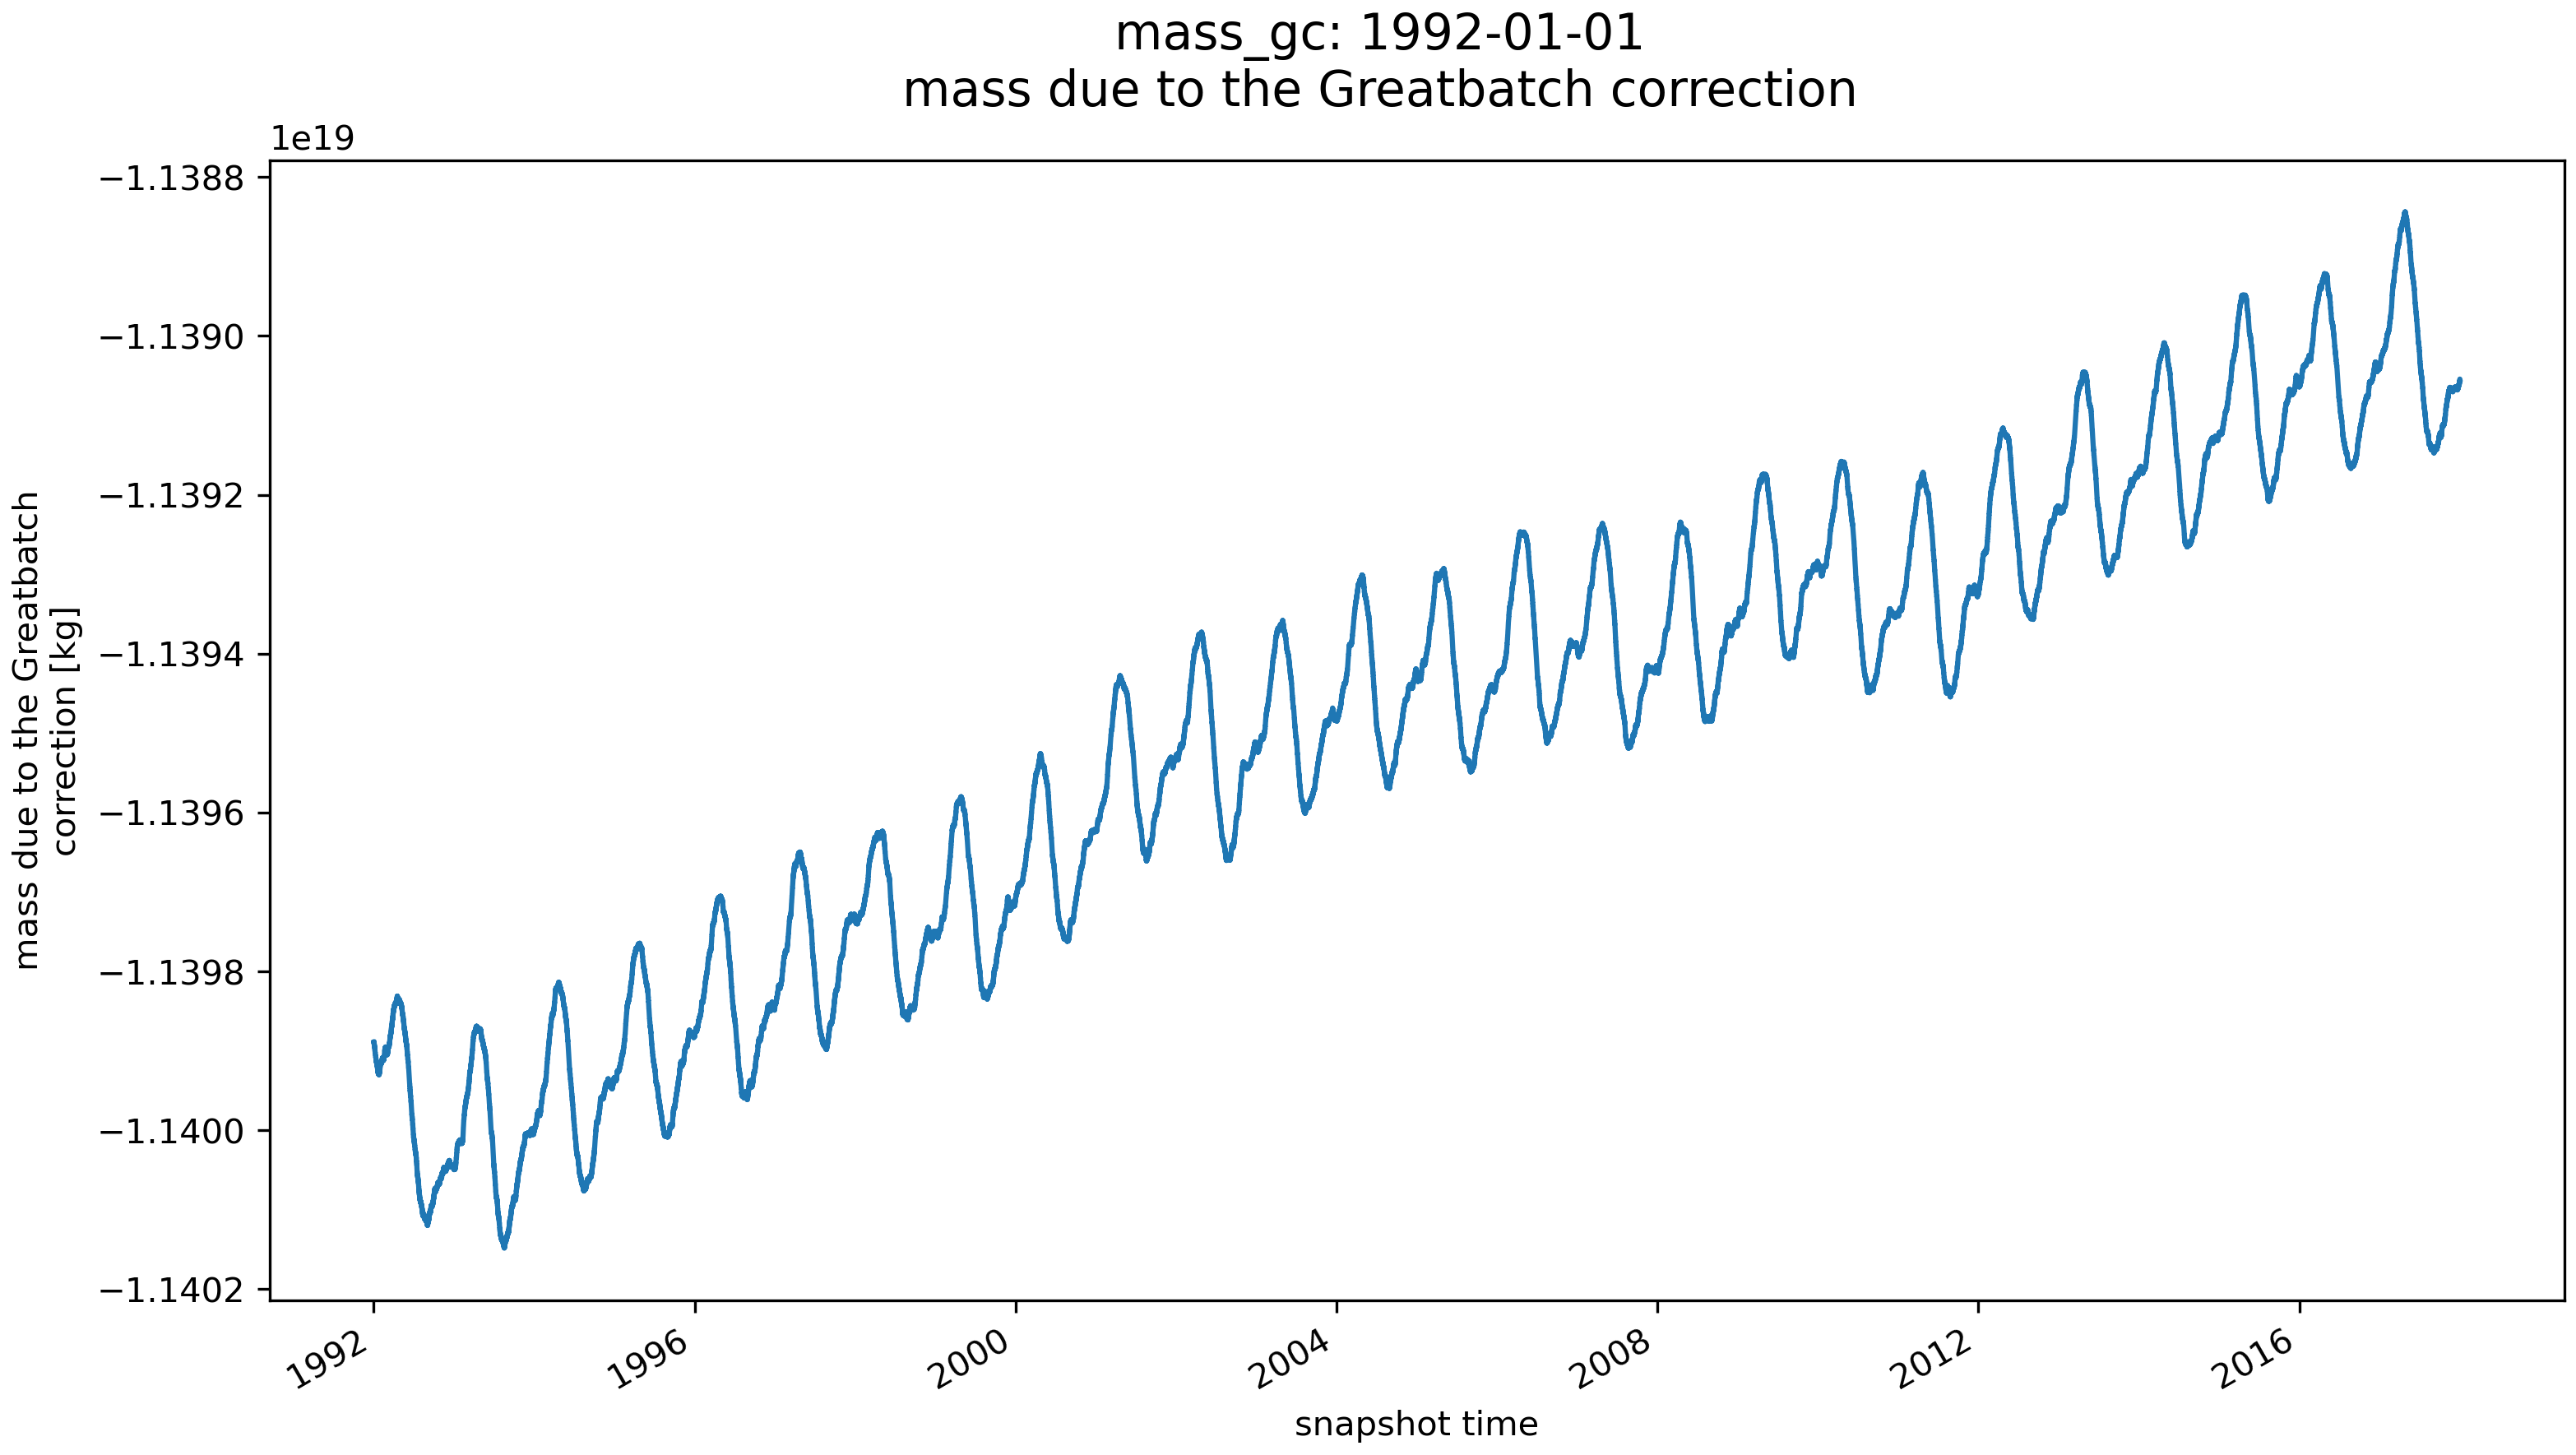
\includegraphics[scale=0.55]{../images/plots/oneD_plots/SBO_Core_Products/mass_gc.png}
\caption{Dataset: SBO\_CORE\_PRODUCTS Variable: mass\_gc}
\label{tab:table-SBO_CORE_PRODUCTS_mass_gc-Plot}
\end{figure}
\pagebreak
\subsubsection{1D Variable mass\_si}
\begin{longtable}{|m{0.06\textwidth}|m{0.41\textwidth}|m{0.39\textwidth}|m{0.06\textwidth}|}
\caption{CDL description of SBO\_CORE\_PRODUCTS's mass\_si variable}
\label{tab:table-SBO_CORE_PRODUCTS_mass_si} \\ 
\hline \endhead \hline \endfoot
\rowcolor{lightgray} \textbf{Storage Type} & \textbf{Variable Name} & \textbf{Description} & \textbf{Unit} \\ \hline
float64 & mass\_si & sea-ice mass & kg \\ \hline
\rowcolor{lightgray}  \multicolumn{4}{|p{1.00\textwidth}|}{\textbf{CDL Description}} \\ \hline
\multicolumn{4}{|p{1.00\textwidth}|}{\makecell{\parbox{1\textwidth}{float64 mass\_si(time)\\
\hspace*{0.5cm}mass\_si: \_FillValue = 9.969209968386869e+36\\
\hspace*{0.5cm}mass\_si: coverage\_content\_type = modelResult\\
\hspace*{0.5cm}mass\_si: long\_name = sea: ice mass\\
\hspace*{0.5cm}mass\_si: units = kg\\
\hspace*{0.5cm}mass\_si: valid\_min = 1.5801085624300974e+16\\
\hspace*{0.5cm}mass\_si: valid\_max = 3.372421224523182e+16\\
\hspace*{0.5cm}mass\_si: coordinates = time}}} \\ \hline
\rowcolor{lightgray} \multicolumn{4}{|p{1.00\textwidth}|}{\textbf{Comments}} \\ \hline
\multicolumn{4}{|p{1\textwidth}|}{N/A} \\ \hline
\end{longtable}

\begin{figure}[H]
\centering
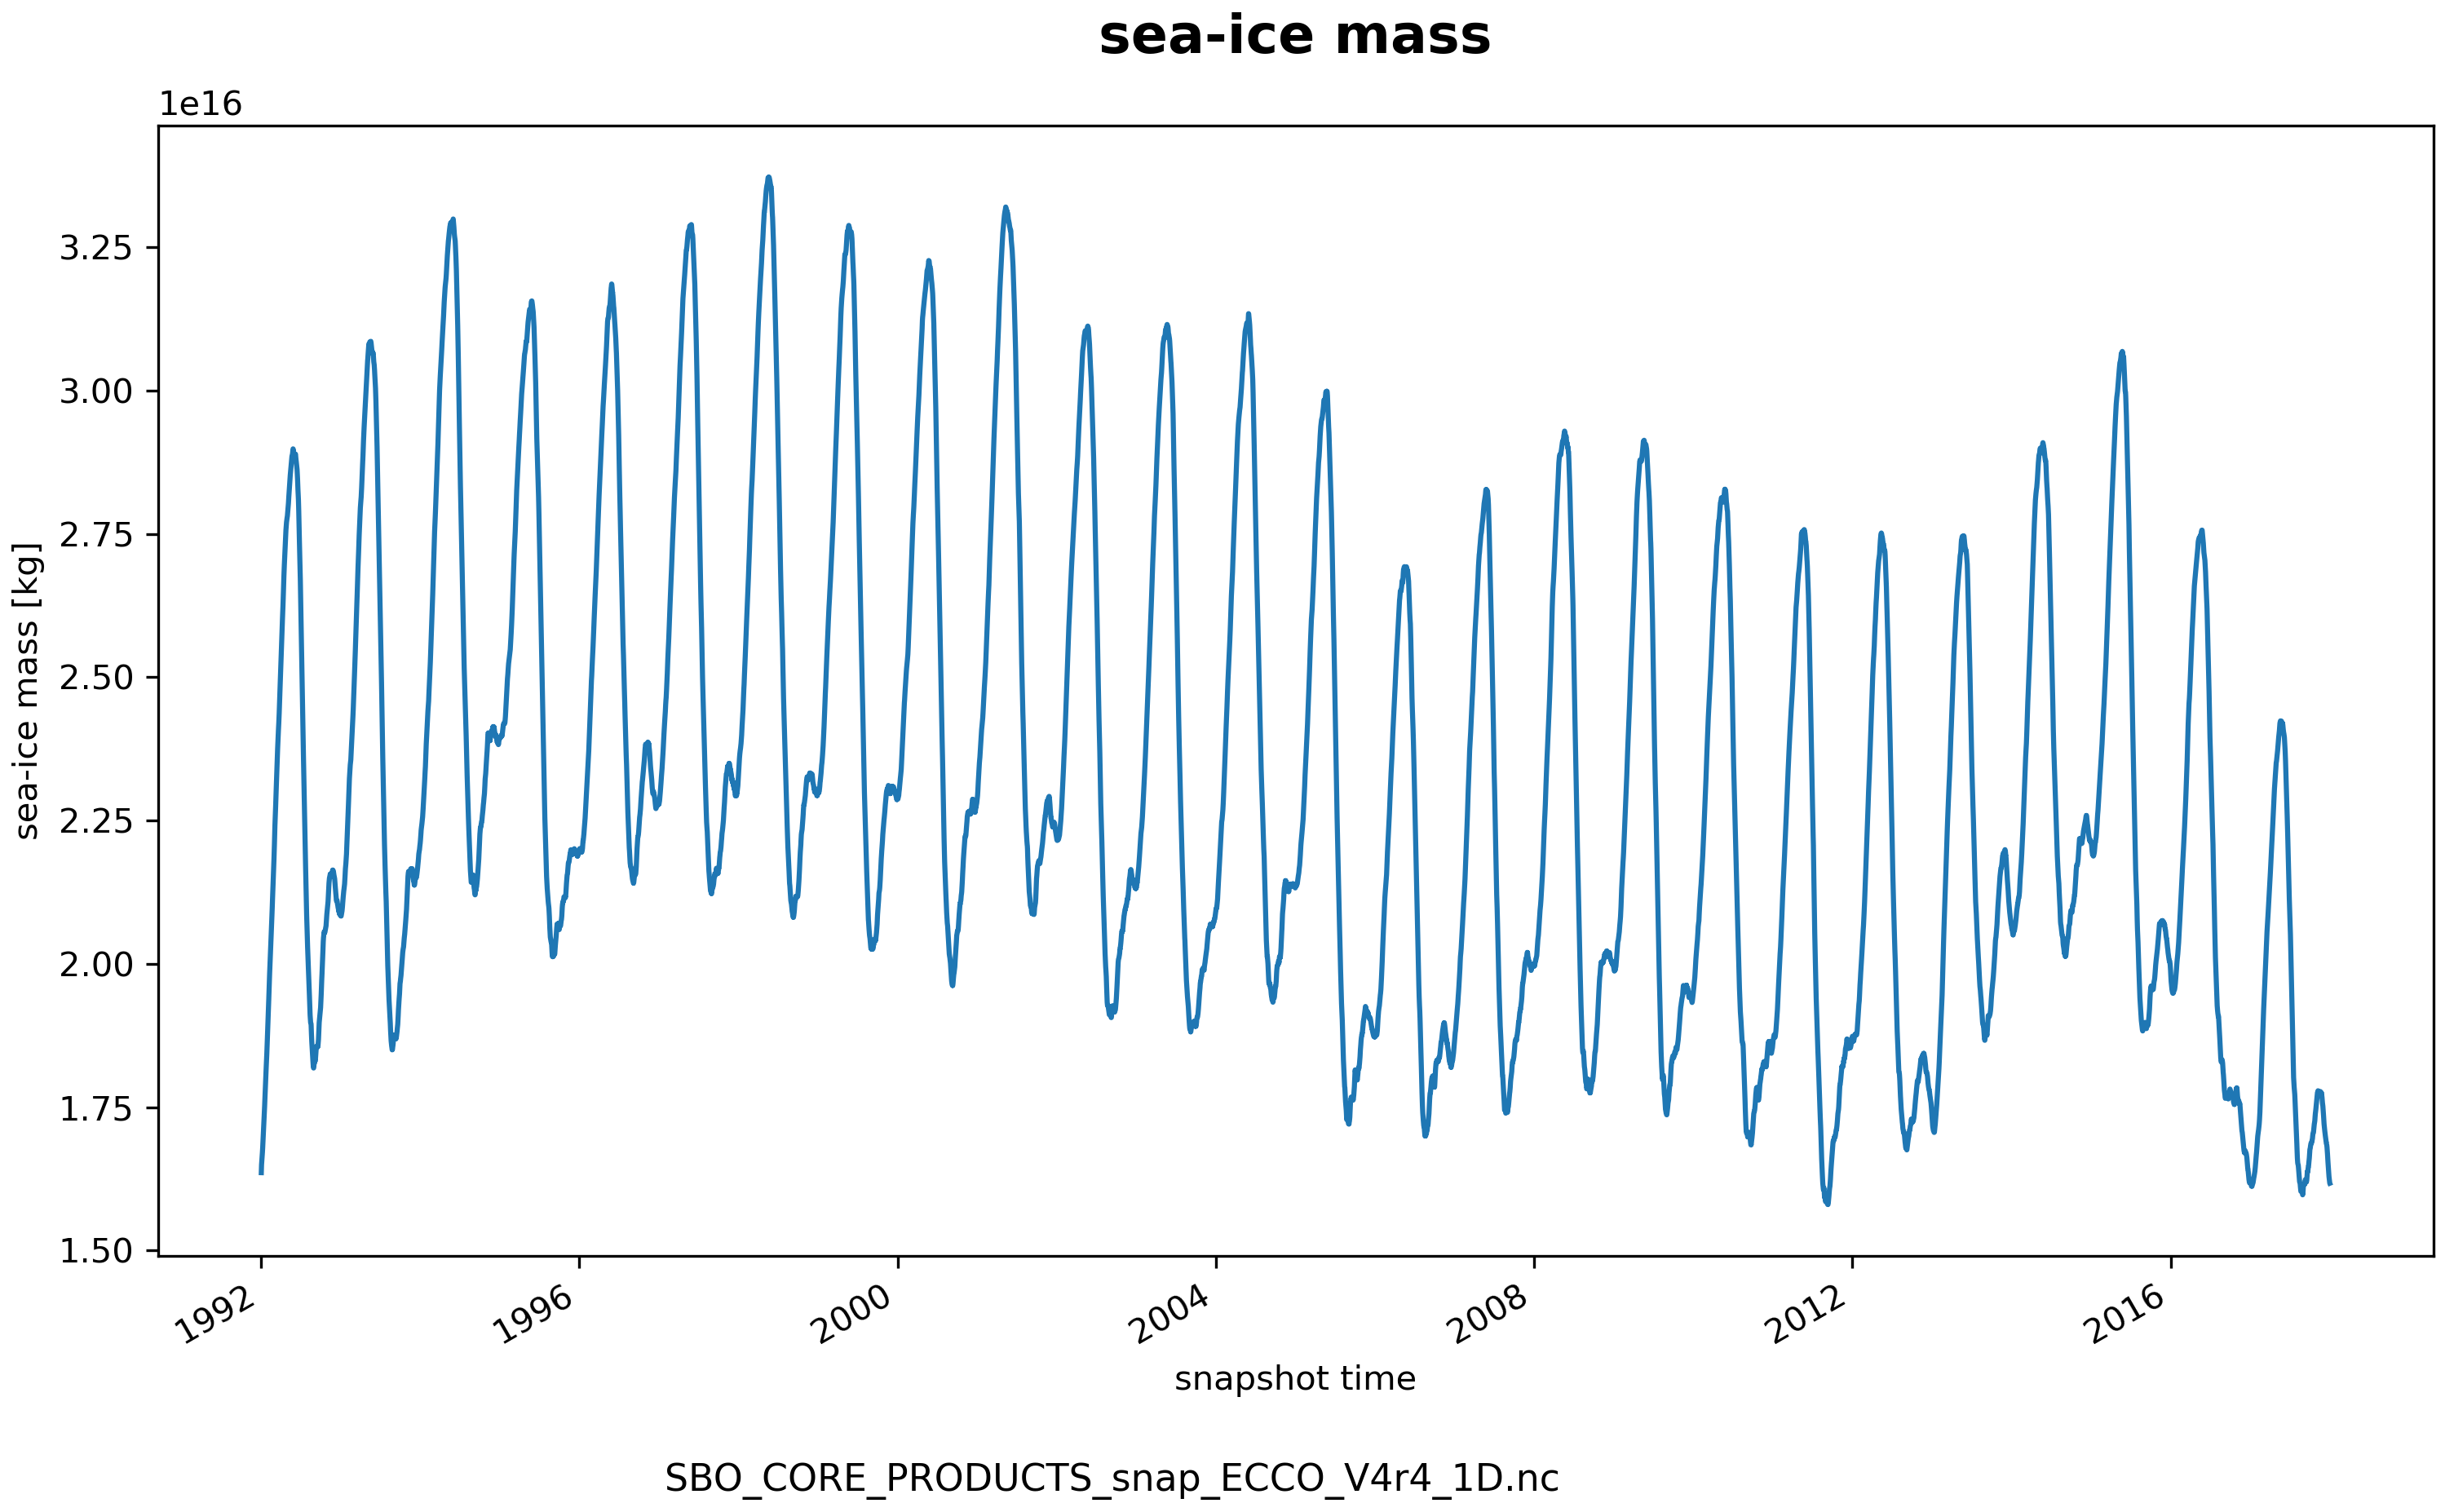
\includegraphics[scale=0.55]{../images/plots/oneD_plots/SBO_Core_Products/mass_si.png}
\caption{Dataset: SBO\_CORE\_PRODUCTS Variable: mass\_si}
\label{tab:table-SBO_CORE_PRODUCTS_mass_si-Plot}
\end{figure}
\pagebreak
\subsubsection{1D Variable sboarea}
\begin{longtable}{|m{0.06\textwidth}|m{0.41\textwidth}|m{0.39\textwidth}|m{0.06\textwidth}|}
\caption{CDL description of SBO\_CORE\_PRODUCTS's sboarea variable}
\label{tab:table-SBO_CORE_PRODUCTS_sboarea} \\ 
\hline \endhead \hline \endfoot
\rowcolor{lightgray} \textbf{Storage Type} & \textbf{Variable Name} & \textbf{Description} & \textbf{Unit} \\ \hline
float64 & sboarea & surface area of oceans & m2 \\ \hline
\rowcolor{lightgray}  \multicolumn{4}{|p{1.00\textwidth}|}{\textbf{CDL Description}} \\ \hline
\multicolumn{4}{|p{1.00\textwidth}|}{\makecell{\parbox{1\textwidth}{float64 sboarea(time)\\
\hspace*{0.5cm}sboarea: \_FillValue = 9.969209968386869e+36\\
\hspace*{0.5cm}sboarea: coverage\_content\_type = modelResult\\
\hspace*{0.5cm}sboarea: long\_name = surface area of oceans\\
\hspace*{0.5cm}sboarea: units = m2\\
\hspace*{0.5cm}sboarea: valid\_min = 358013861149443.5\\
\hspace*{0.5cm}sboarea: valid\_max = 358013861149443.5\\
\hspace*{0.5cm}sboarea: coordinates = time}}} \\ \hline
\rowcolor{lightgray} \multicolumn{4}{|p{1.00\textwidth}|}{\textbf{Comments}} \\ \hline
\multicolumn{4}{|p{1\textwidth}|}{Note: ocean surface area is constant but provided as time series for convenience} \\ \hline
\end{longtable}

\begin{figure}[H]
\centering
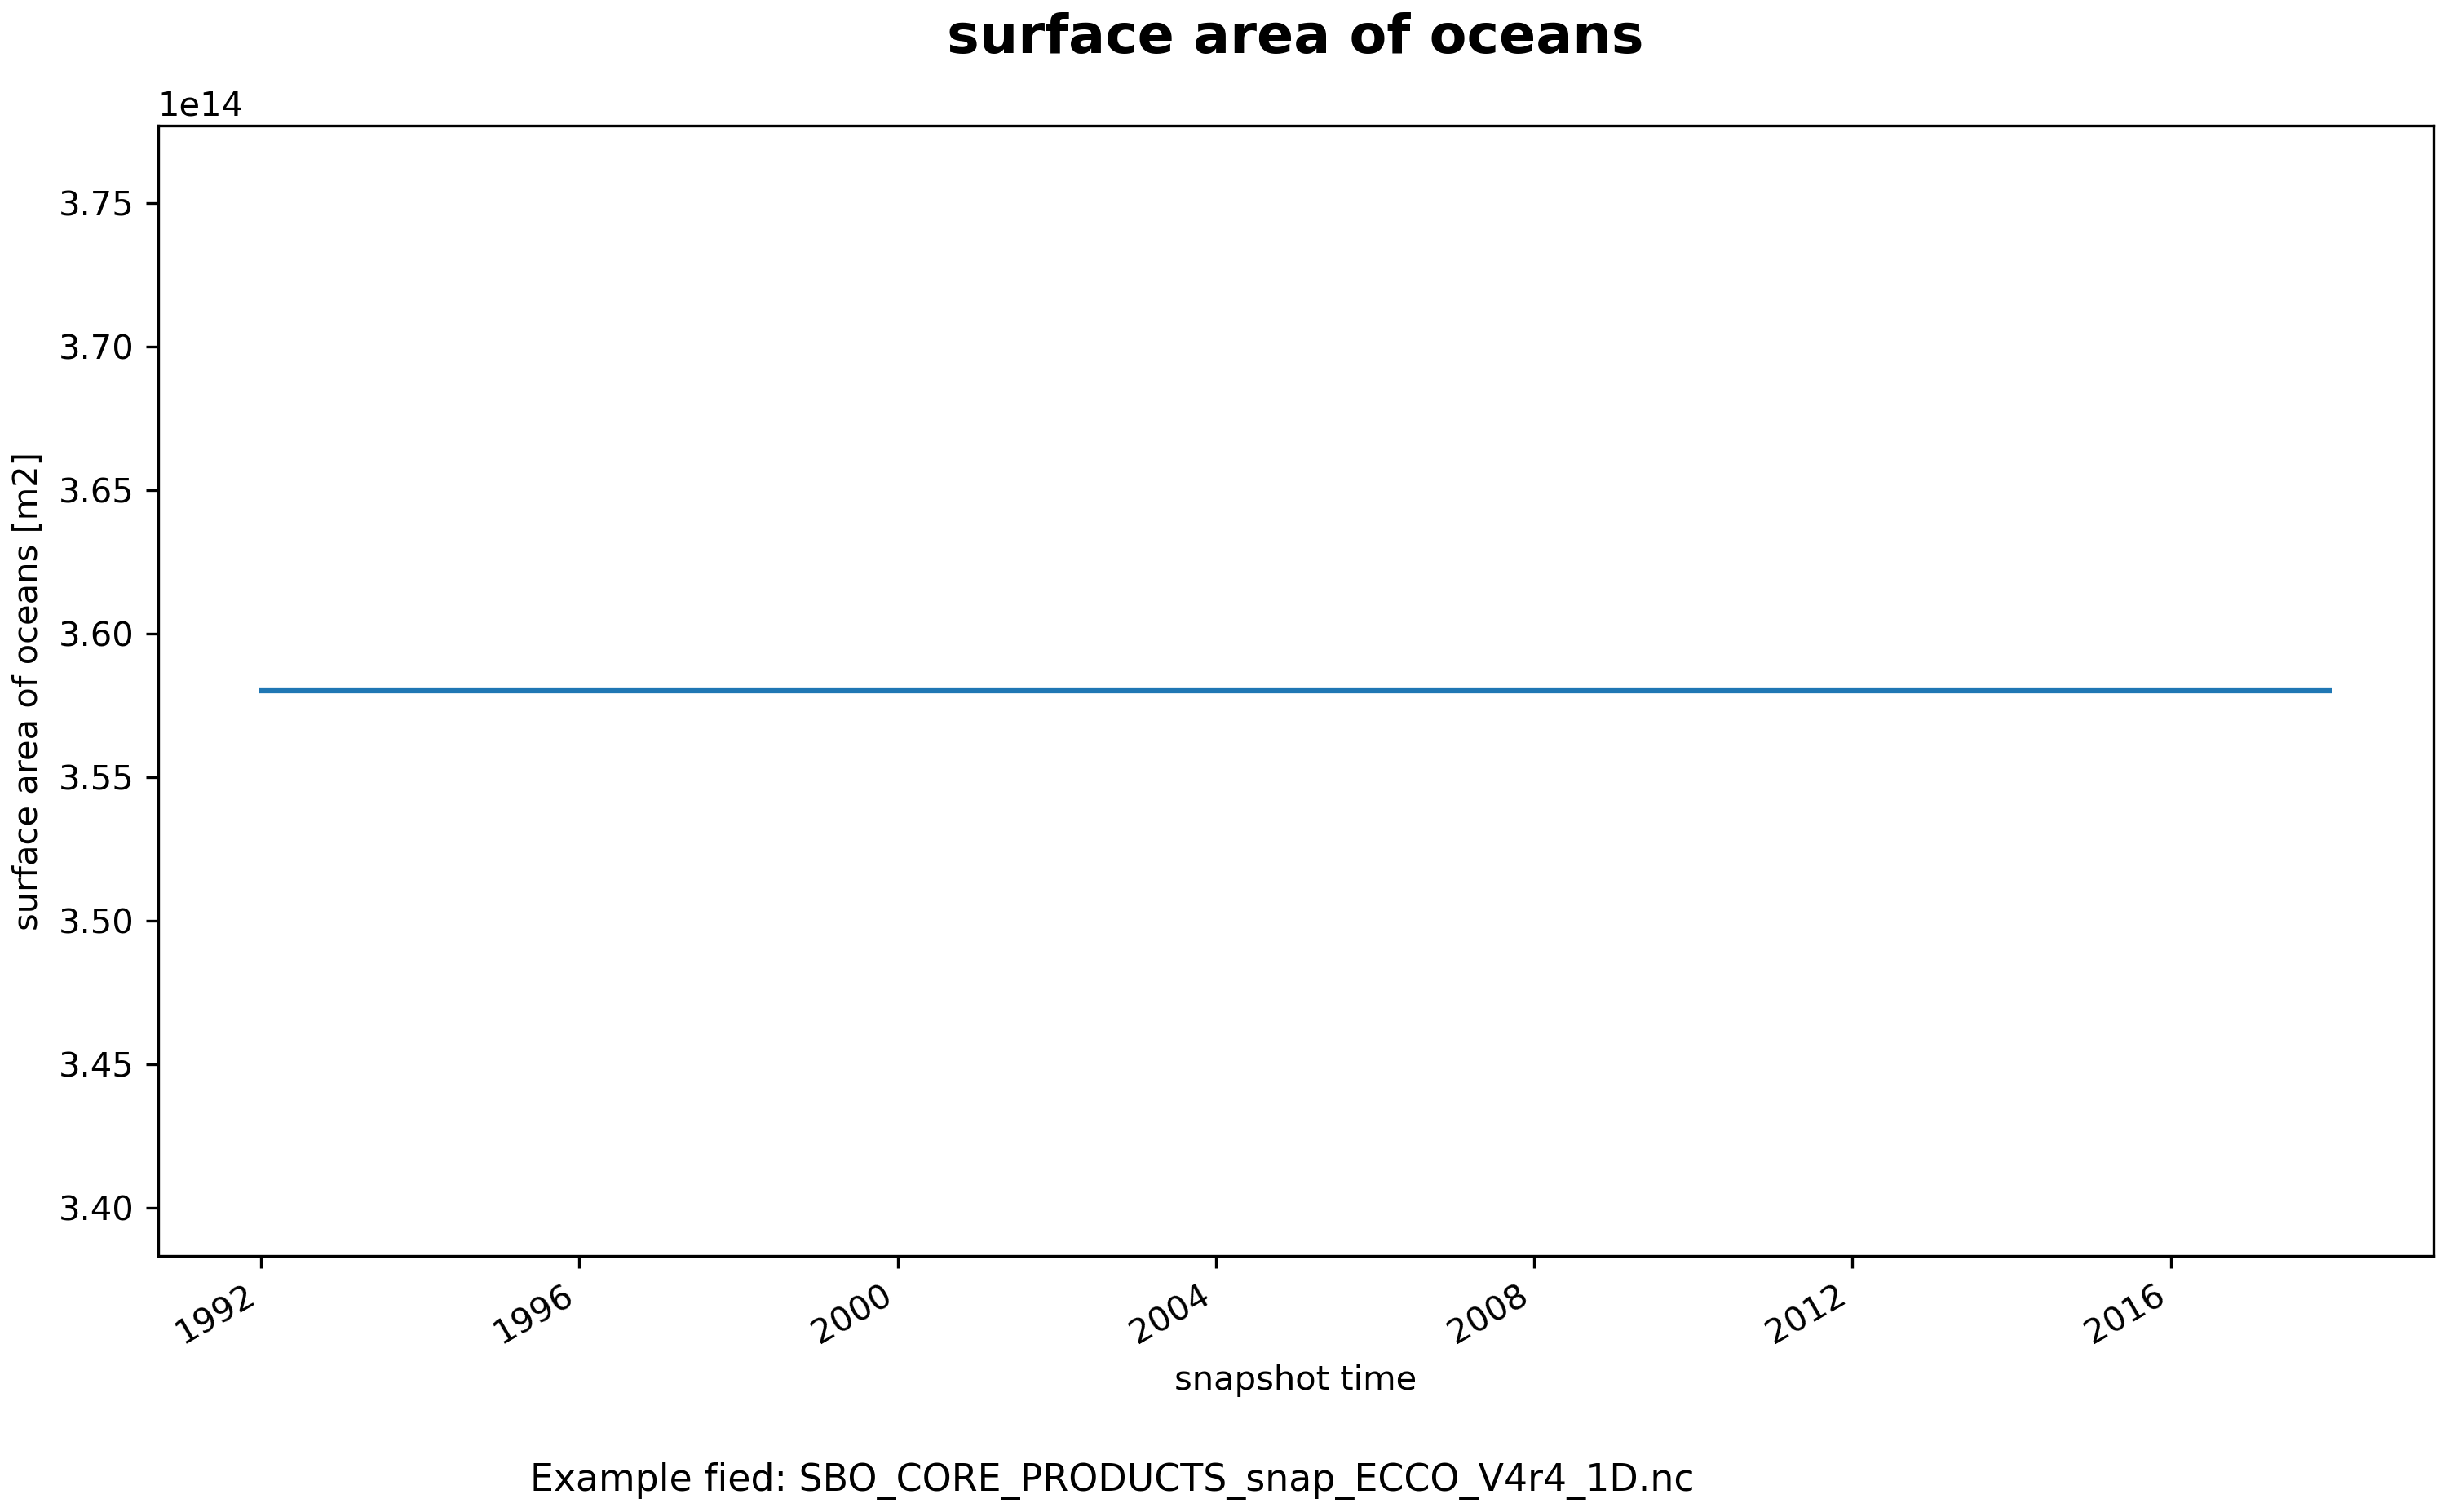
\includegraphics[scale=0.55]{../images/plots/oneD_plots/SBO_Core_Products/sboarea.png}
\caption{Dataset: SBO\_CORE\_PRODUCTS Variable: sboarea}
\label{tab:table-SBO_CORE_PRODUCTS_sboarea-Plot}
\end{figure}
\pagebreak
\subsubsection{1D Variable xcom}
\begin{longtable}{|m{0.06\textwidth}|m{0.41\textwidth}|m{0.39\textwidth}|m{0.06\textwidth}|}
\caption{CDL description of SBO\_CORE\_PRODUCTS's xcom variable}
\label{tab:table-SBO_CORE_PRODUCTS_xcom} \\ 
\hline \endhead \hline \endfoot
\rowcolor{lightgray} \textbf{Storage Type} & \textbf{Variable Name} & \textbf{Description} & \textbf{Unit} \\ \hline
float64 & xcom & x-comp of center-of-mass of ocean & m \\ \hline
\rowcolor{lightgray}  \multicolumn{4}{|p{1.00\textwidth}|}{\textbf{CDL Description}} \\ \hline
\multicolumn{4}{|p{1.00\textwidth}|}{\makecell{\parbox{1\textwidth}{float64 xcom(time)\\
\hspace*{0.5cm}xcom: \_FillValue = 9.969209968386869e+36\\
\hspace*{0.5cm}xcom: coverage\_content\_type = modelResult\\
\hspace*{0.5cm}xcom: long\_name = x: comp of center: of: mass of ocean\\
\hspace*{0.5cm}xcom: units = m\\
\hspace*{0.5cm}xcom: valid\_min = : 763730.0399730895\\
\hspace*{0.5cm}xcom: valid\_max = : 763667.0104211655\\
\hspace*{0.5cm}xcom: coordinates = time}}} \\ \hline
\rowcolor{lightgray} \multicolumn{4}{|p{1.00\textwidth}|}{\textbf{Comments}} \\ \hline
\multicolumn{4}{|p{1\textwidth}|}{N/A} \\ \hline
\end{longtable}

\begin{figure}[H]
\centering
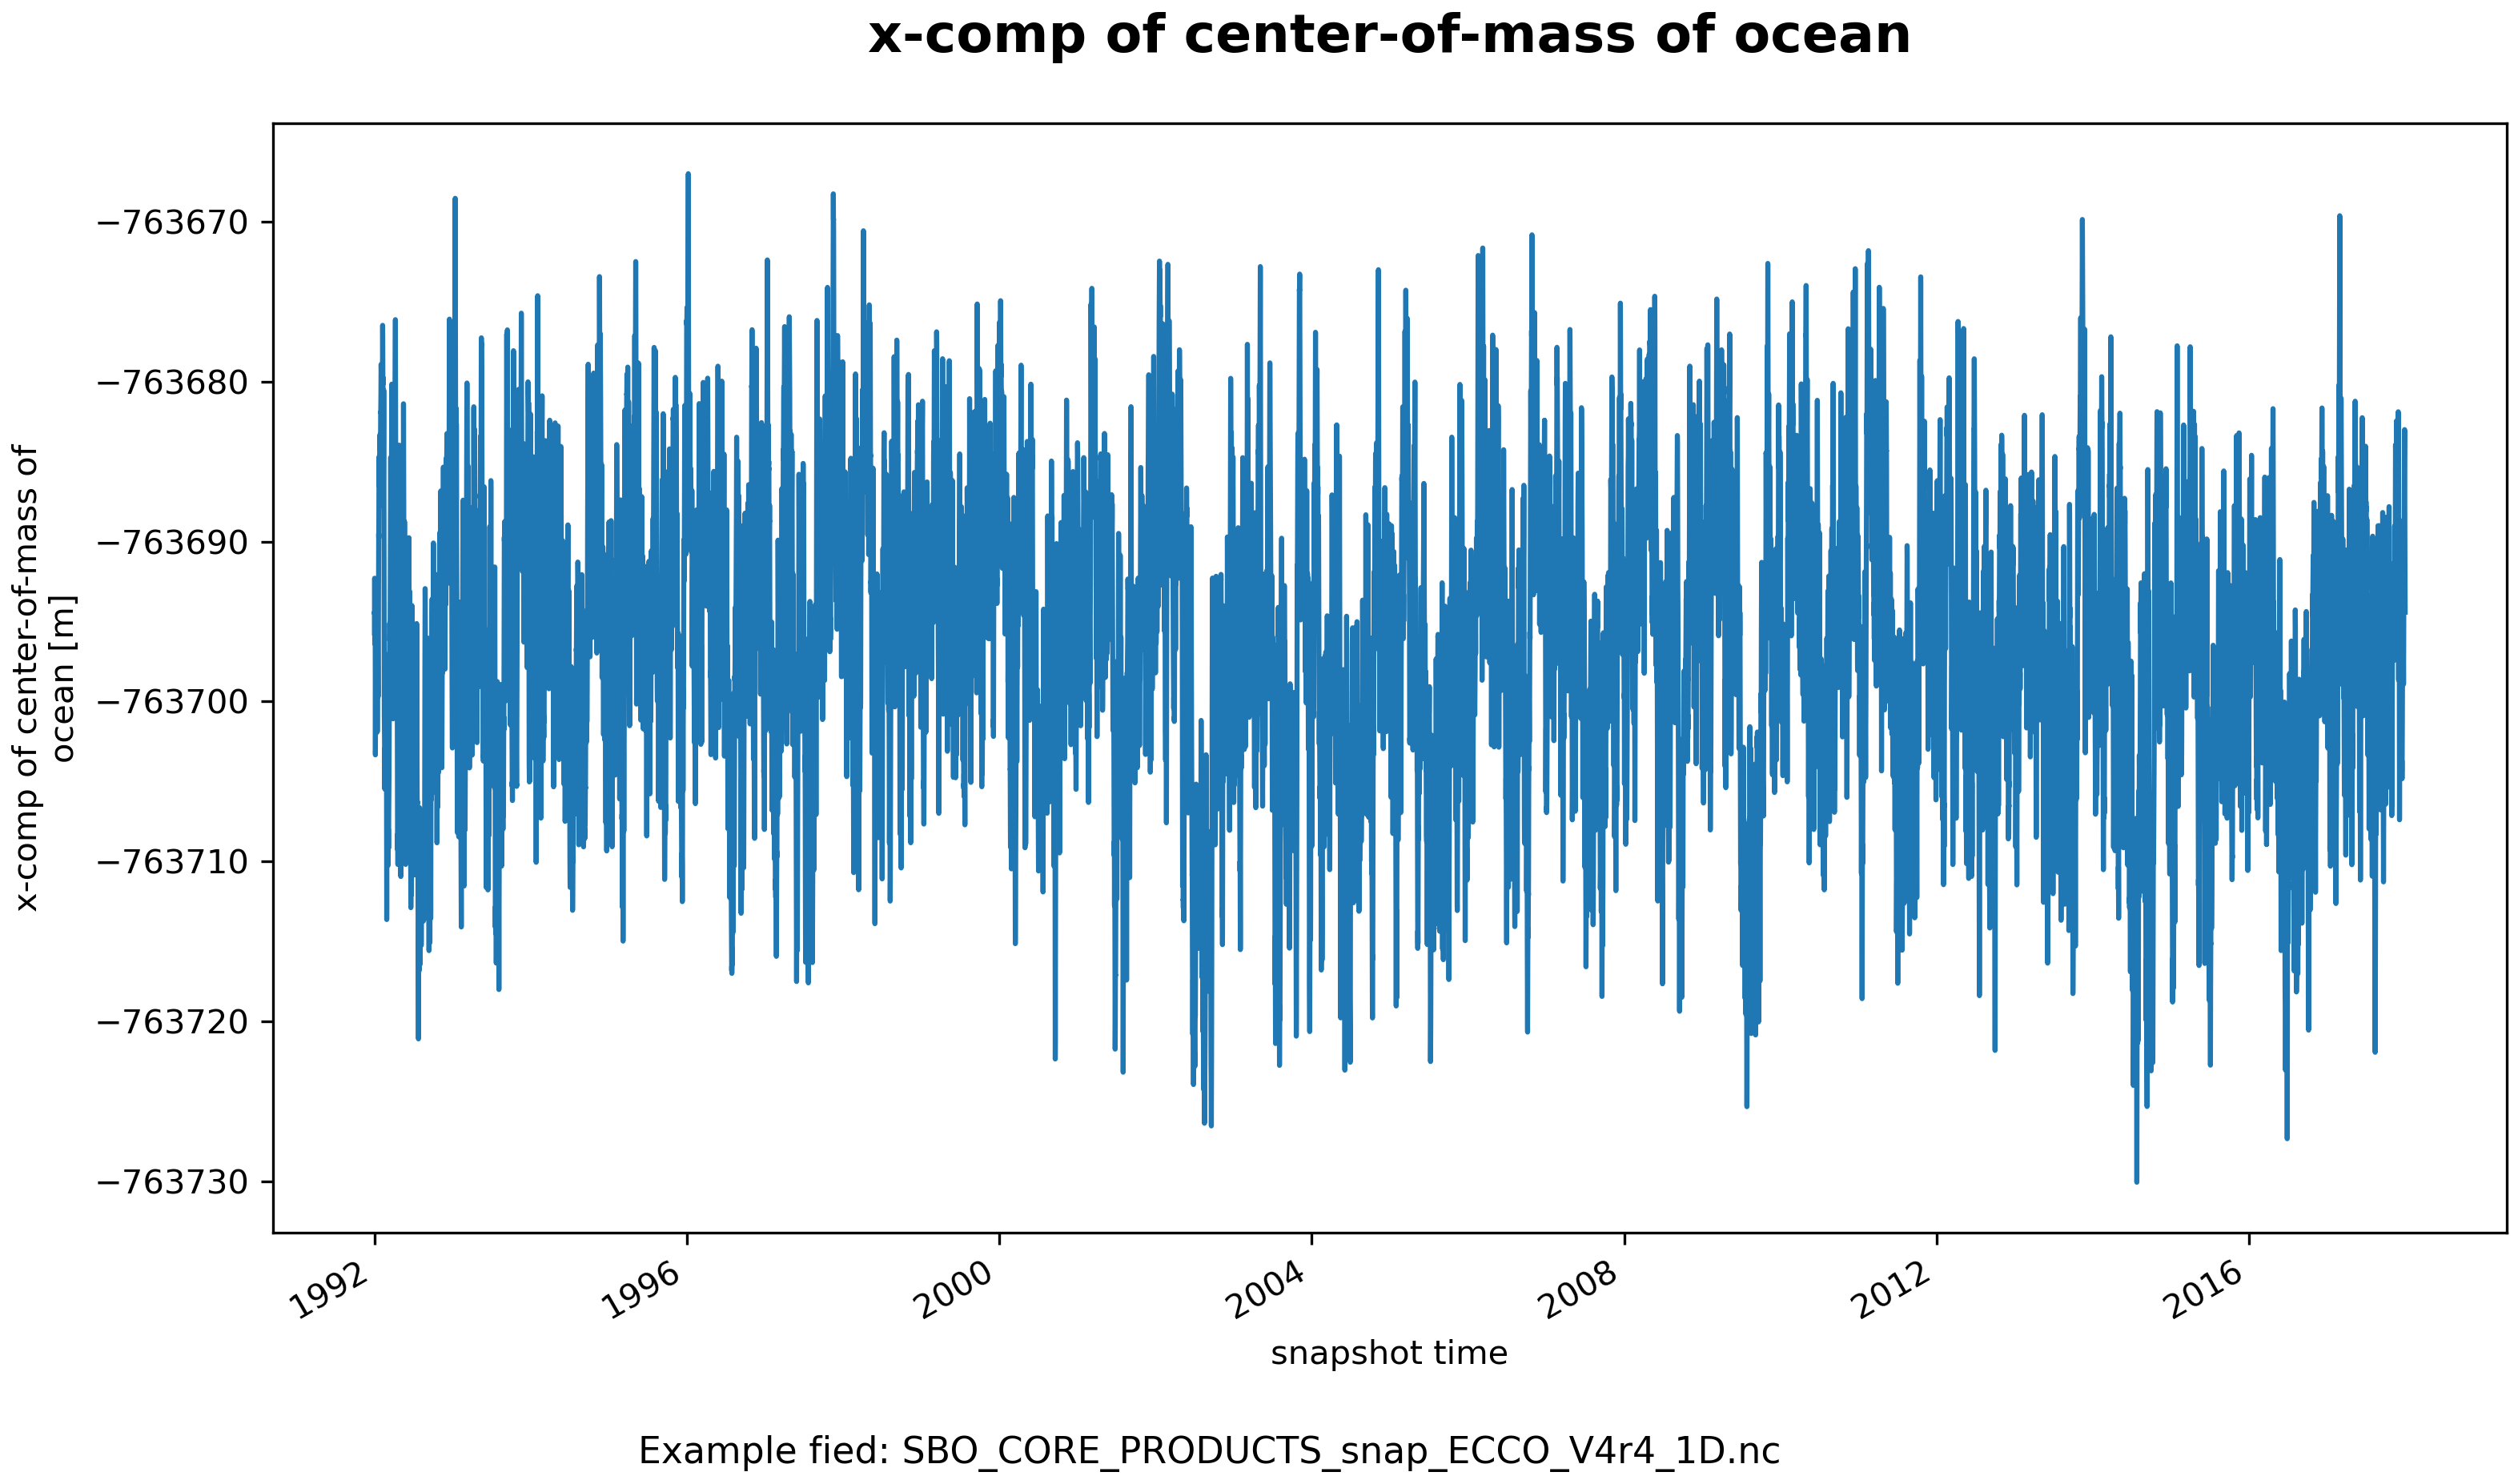
\includegraphics[scale=0.55]{../images/plots/oneD_plots/SBO_Core_Products/xcom.png}
\caption{Dataset: SBO\_CORE\_PRODUCTS Variable: xcom}
\label{tab:table-SBO_CORE_PRODUCTS_xcom-Plot}
\end{figure}
\pagebreak
\subsubsection{1D Variable xcom\_fw}
\begin{longtable}{|m{0.06\textwidth}|m{0.41\textwidth}|m{0.39\textwidth}|m{0.06\textwidth}|}
\caption{CDL description of SBO\_CORE\_PRODUCTS's xcom\_fw variable}
\label{tab:table-SBO_CORE_PRODUCTS_xcom_fw} \\ 
\hline \endhead \hline \endfoot
\rowcolor{lightgray} \textbf{Storage Type} & \textbf{Variable Name} & \textbf{Description} & \textbf{Unit} \\ \hline
float64 & xcom\_fw & x-comp of center-of-mass of freshwater flux & m \\ \hline
\rowcolor{lightgray}  \multicolumn{4}{|p{1.00\textwidth}|}{\textbf{CDL Description}} \\ \hline
\multicolumn{4}{|p{1.00\textwidth}|}{\makecell{\parbox{1\textwidth}{float64 xcom\_fw(time)\\
\hspace*{0.5cm}xcom\_fw: \_FillValue = 9.969209968386869e+36\\
\hspace*{0.5cm}xcom\_fw: coverage\_content\_type = modelResult\\
\hspace*{0.5cm}xcom\_fw: long\_name = x: comp of center: of: mass of freshwater flux\\
\hspace*{0.5cm}xcom\_fw: units = m\\
\hspace*{0.5cm}xcom\_fw: valid\_min = : 573864.6948562702\\
\hspace*{0.5cm}xcom\_fw: valid\_max = : 573864.6948562652\\
\hspace*{0.5cm}xcom\_fw: coordinates = time}}} \\ \hline
\rowcolor{lightgray} \multicolumn{4}{|p{1.00\textwidth}|}{\textbf{Comments}} \\ \hline
\multicolumn{4}{|p{1\textwidth}|}{N/A} \\ \hline
\end{longtable}

\begin{figure}[H]
\centering
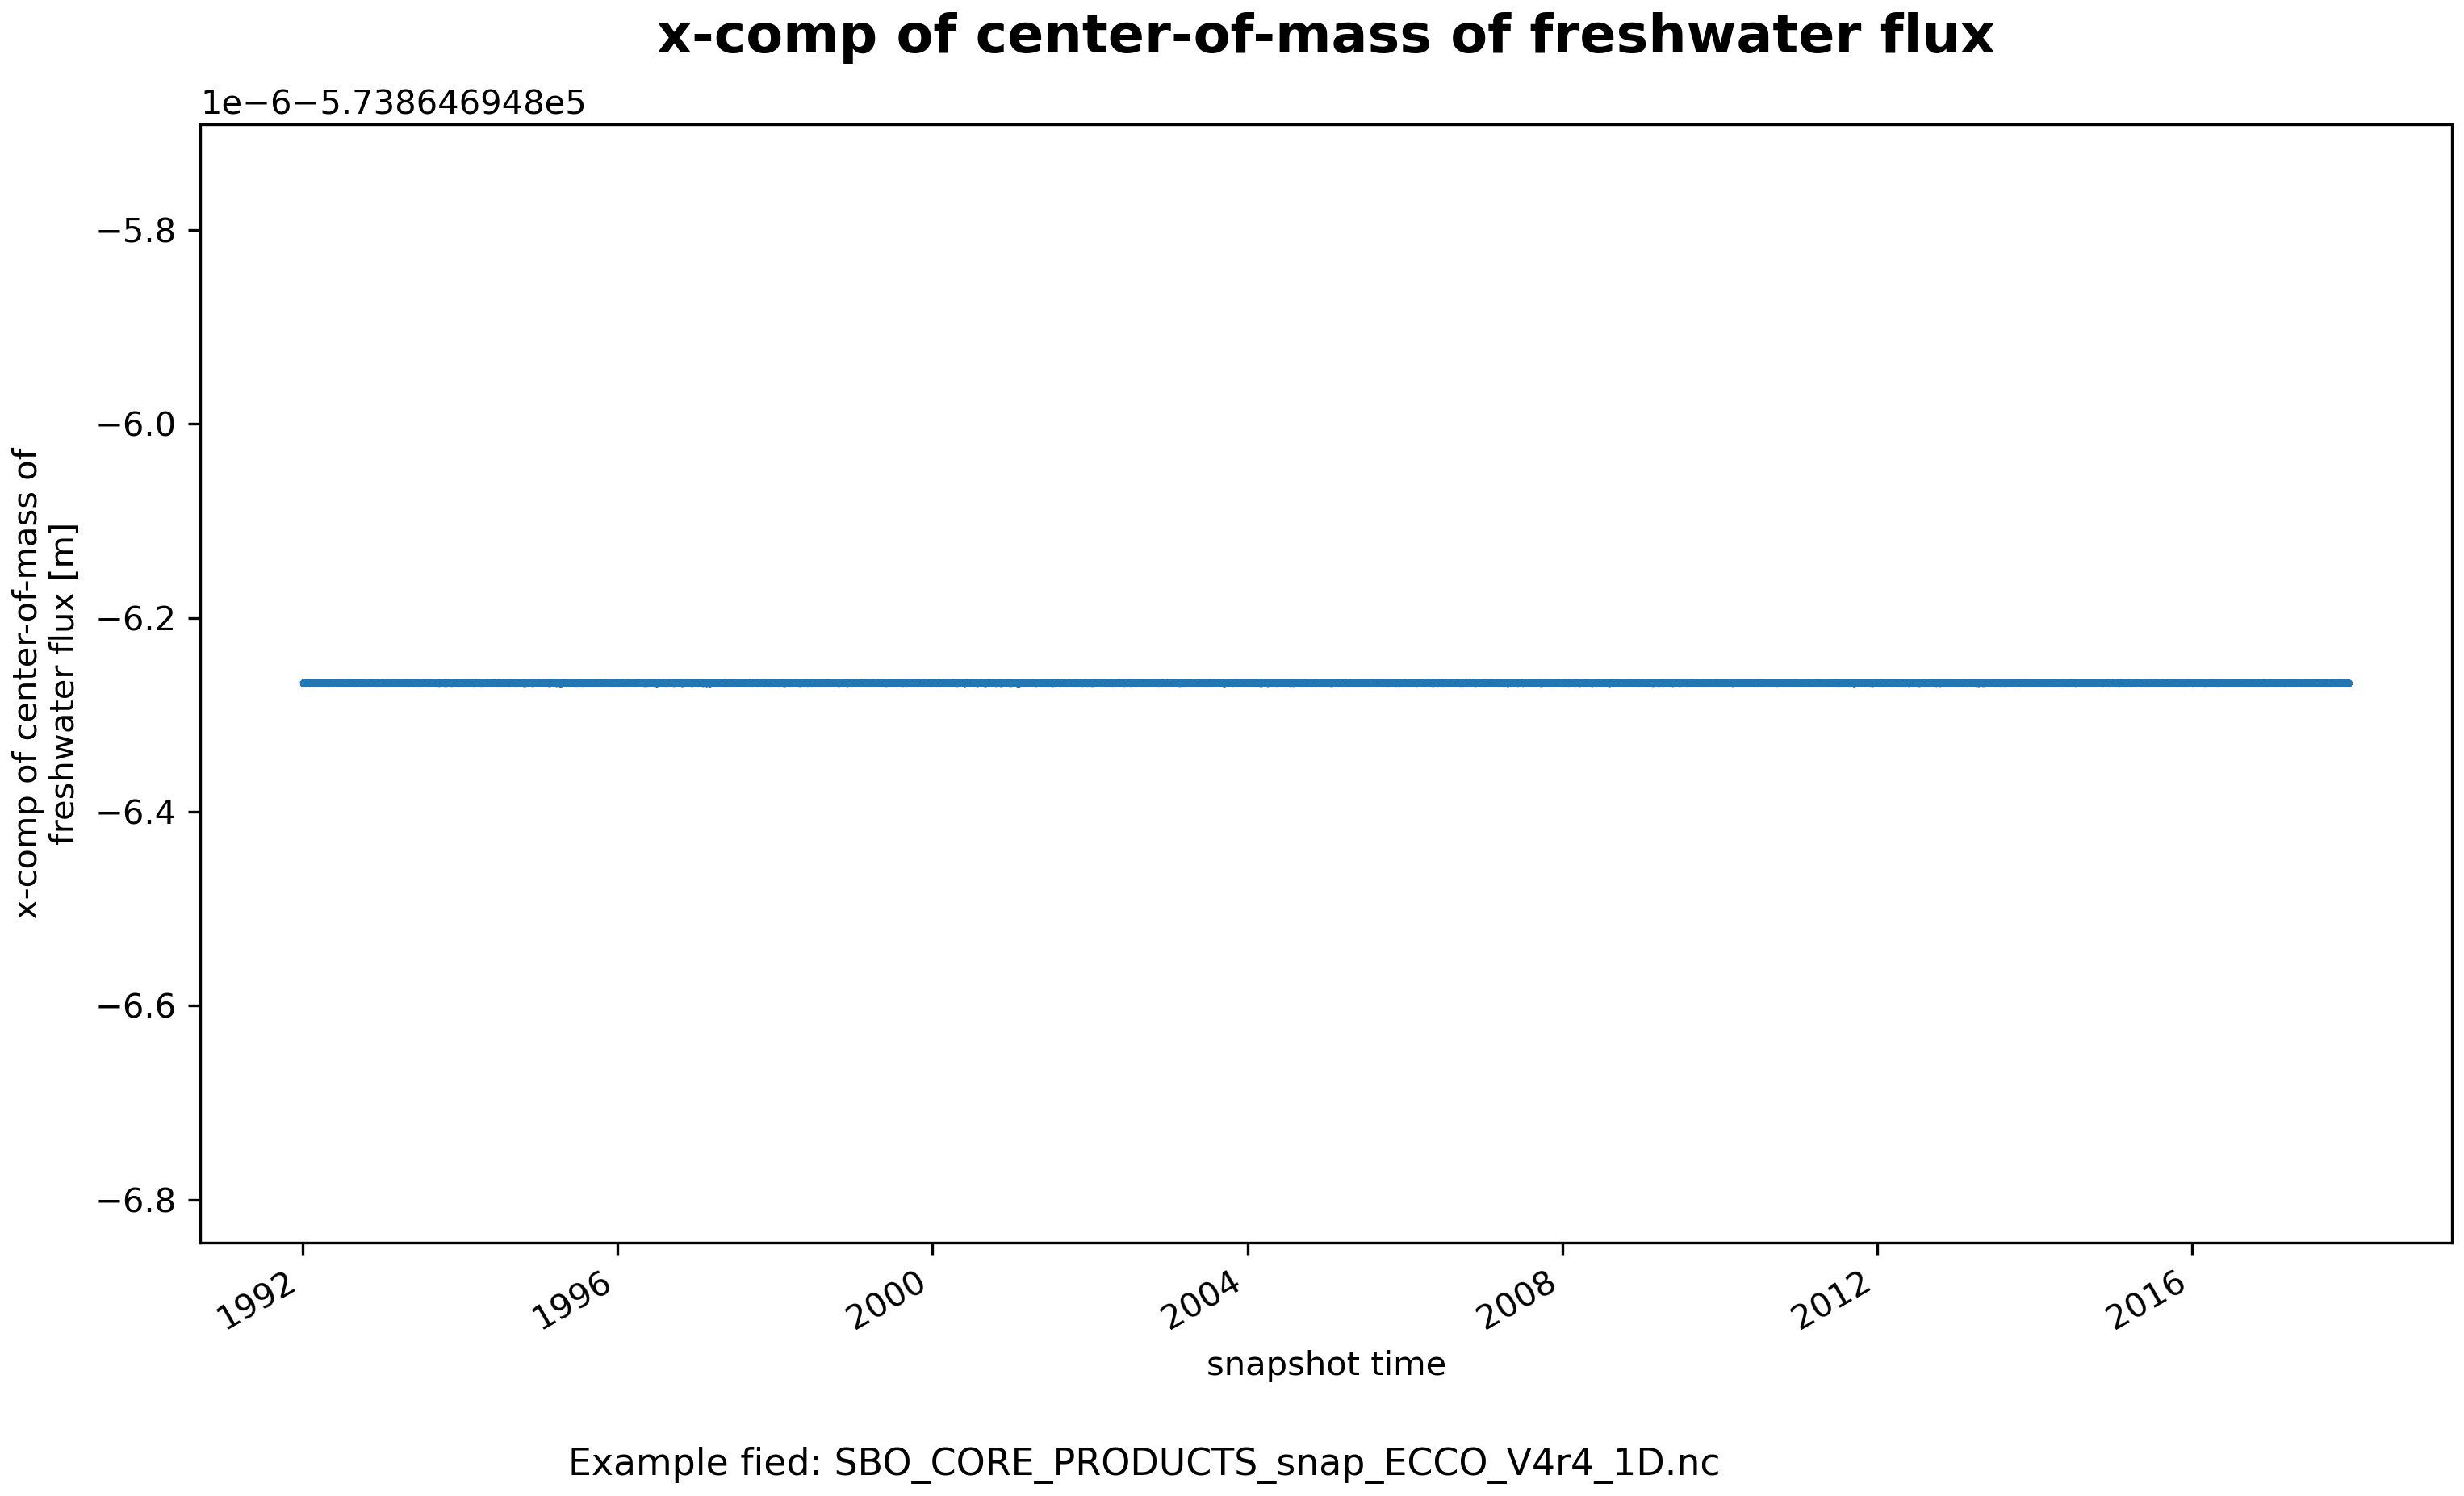
\includegraphics[scale=0.55]{../images/plots/oneD_plots/SBO_Core_Products/xcom_fw.png}
\caption{Dataset: SBO\_CORE\_PRODUCTS Variable: xcom\_fw}
\label{tab:table-SBO_CORE_PRODUCTS_xcom_fw-Plot}
\end{figure}
\pagebreak
\subsubsection{1D Variable xoamc}
\begin{longtable}{|m{0.06\textwidth}|m{0.41\textwidth}|m{0.39\textwidth}|m{0.06\textwidth}|}
\caption{CDL description of SBO\_CORE\_PRODUCTS's xoamc variable}
\label{tab:table-SBO_CORE_PRODUCTS_xoamc} \\ 
\hline \endhead \hline \endfoot
\rowcolor{lightgray} \textbf{Storage Type} & \textbf{Variable Name} & \textbf{Description} & \textbf{Unit} \\ \hline
float64 & xoamc & x-comp of oceanic angular momentum due to currents & kg m2 s-1 \\ \hline
\rowcolor{lightgray}  \multicolumn{4}{|p{1.00\textwidth}|}{\textbf{CDL Description}} \\ \hline
\multicolumn{4}{|p{1.00\textwidth}|}{\makecell{\parbox{1\textwidth}{float64 xoamc(time)\\
\hspace*{0.5cm}xoamc: \_FillValue = 9.969209968386869e+36\\
\hspace*{0.5cm}xoamc: coverage\_content\_type = modelResult\\
\hspace*{0.5cm}xoamc: long\_name = x: comp of oceanic angular momentum due to currents\\
\hspace*{0.5cm}xoamc: units = kg m2 s: 1\\
\hspace*{0.5cm}xoamc: valid\_min = : 3.783733447704127e+24\\
\hspace*{0.5cm}xoamc: valid\_max = 2.555331552045857e+24\\
\hspace*{0.5cm}xoamc: coordinates = time}}} \\ \hline
\rowcolor{lightgray} \multicolumn{4}{|p{1.00\textwidth}|}{\textbf{Comments}} \\ \hline
\multicolumn{4}{|p{1\textwidth}|}{N/A} \\ \hline
\end{longtable}

\begin{figure}[H]
\centering
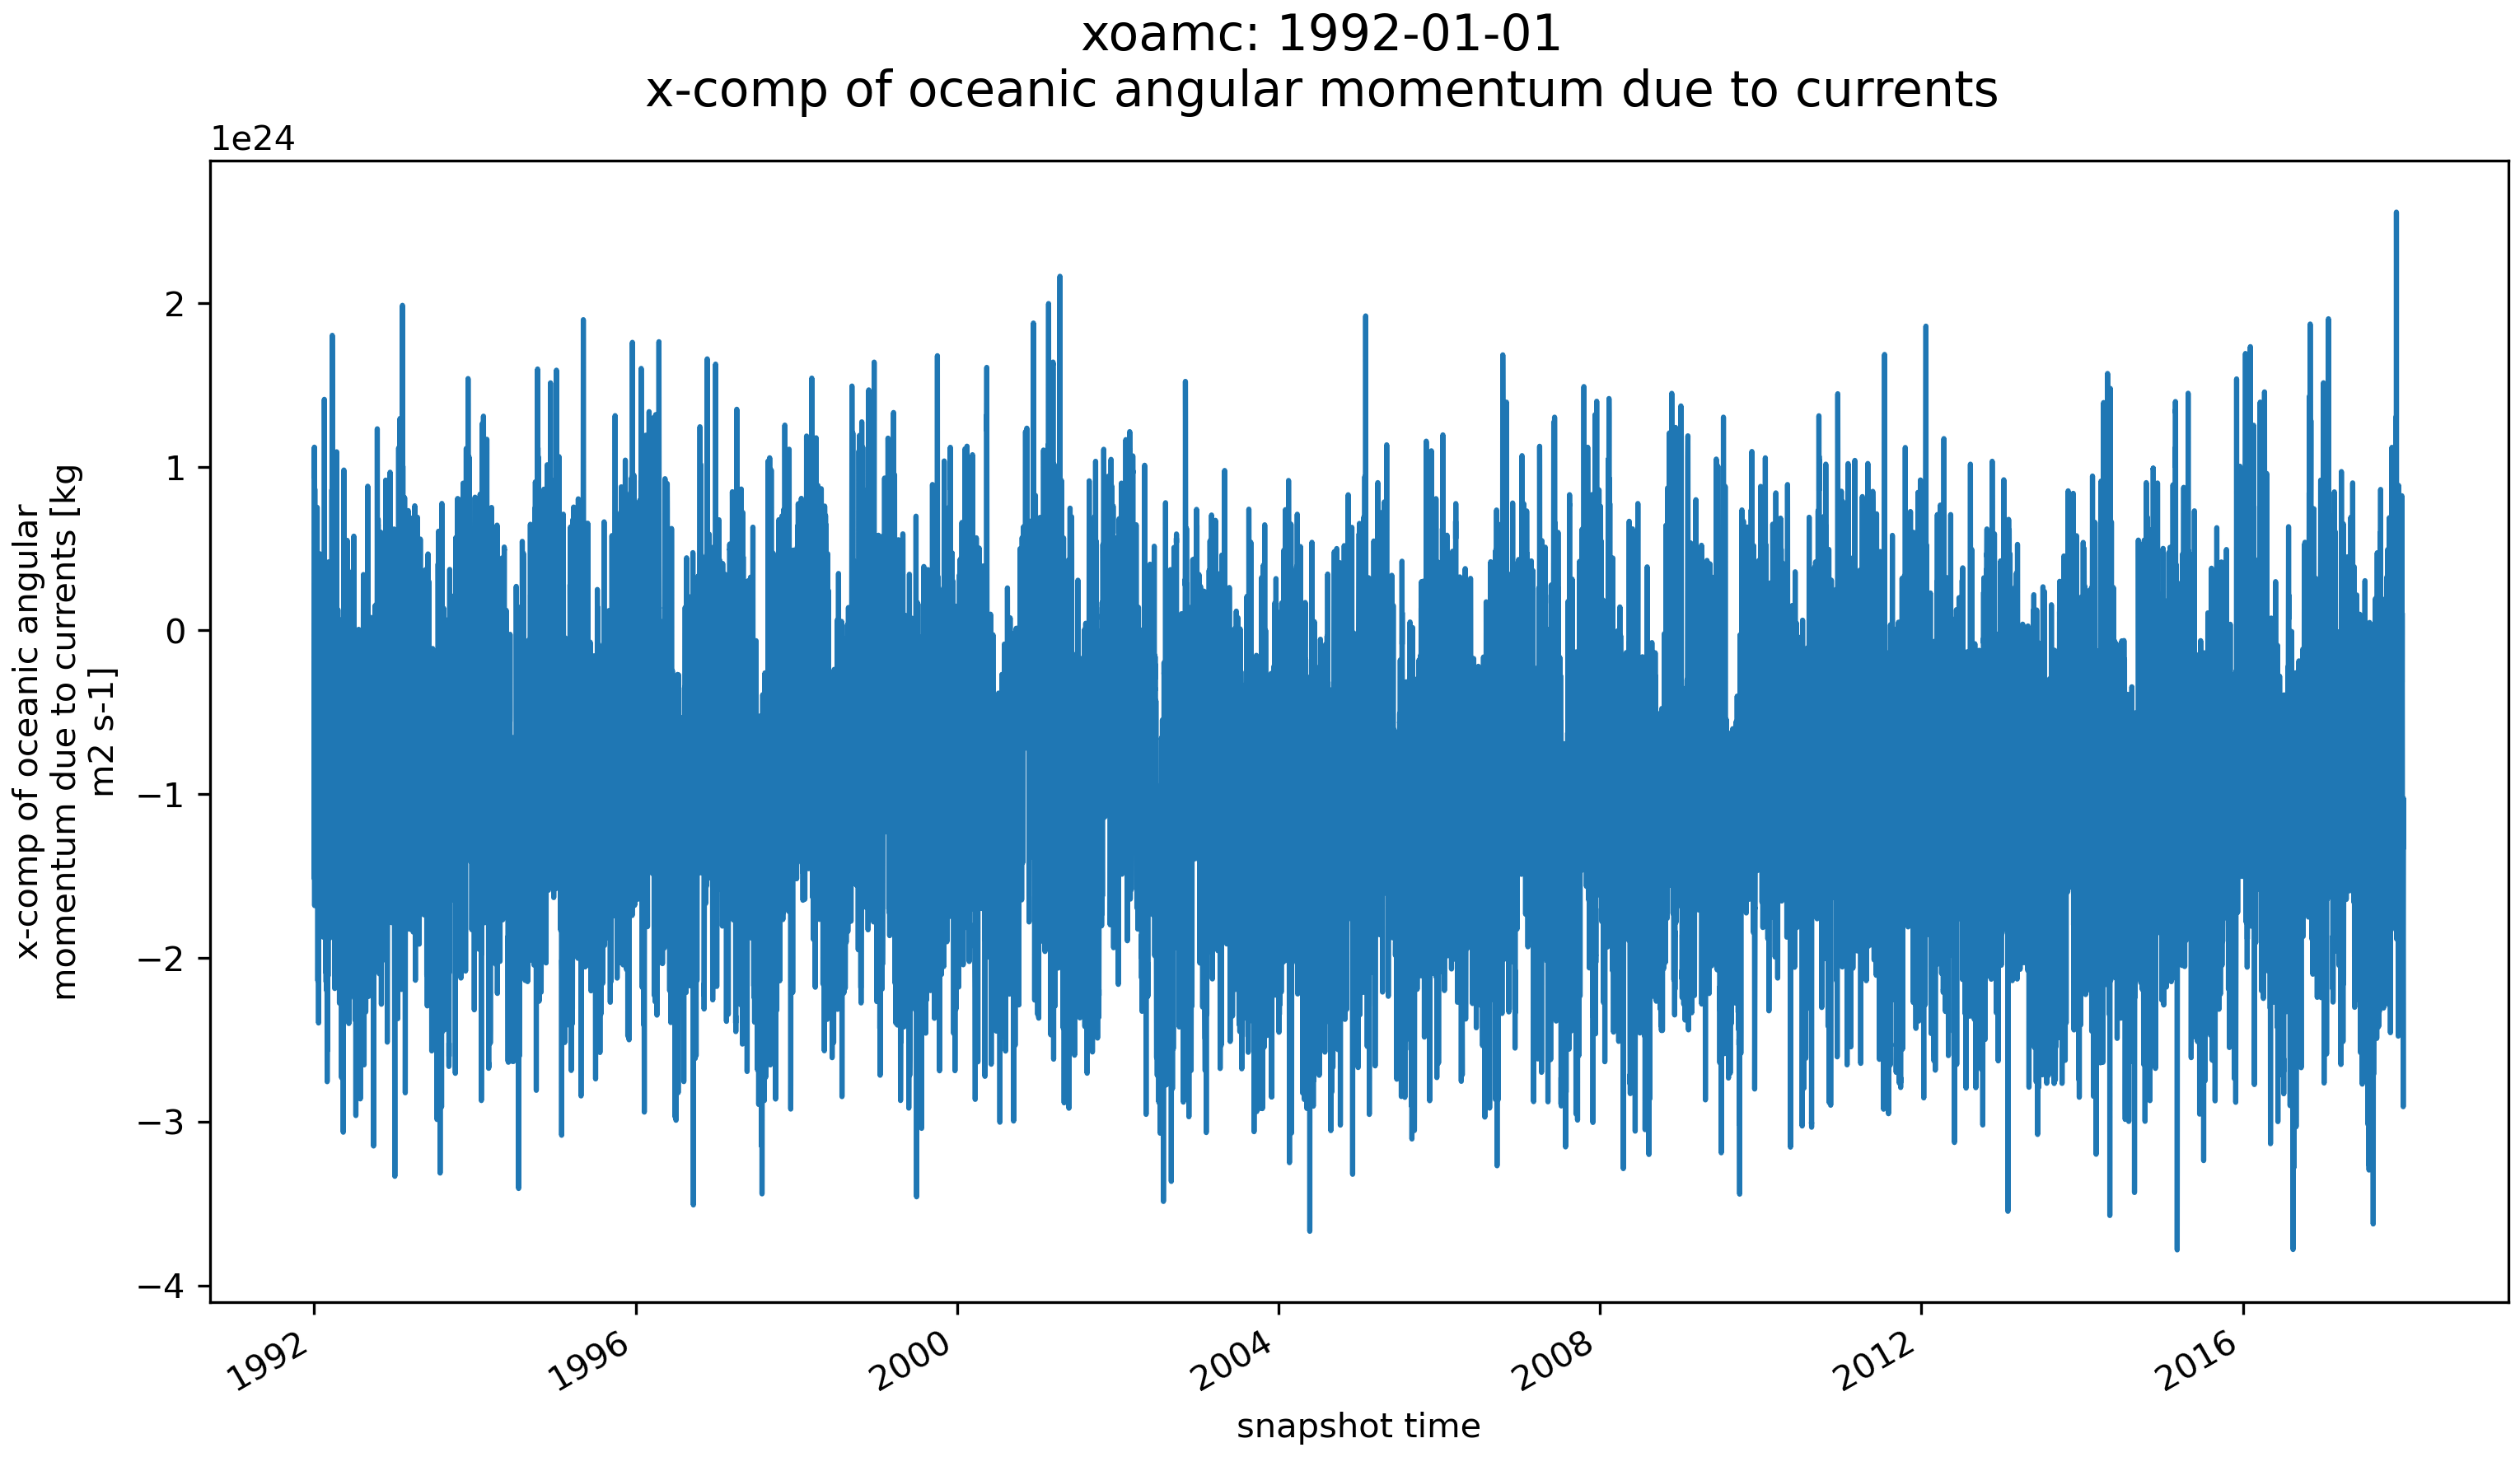
\includegraphics[scale=0.55]{../images/plots/oneD_plots/SBO_Core_Products/xoamc.png}
\caption{Dataset: SBO\_CORE\_PRODUCTS Variable: xoamc}
\label{tab:table-SBO_CORE_PRODUCTS_xoamc-Plot}
\end{figure}
\pagebreak
\subsubsection{1D Variable xoamc\_si}
\begin{longtable}{|m{0.06\textwidth}|m{0.41\textwidth}|m{0.39\textwidth}|m{0.06\textwidth}|}
\caption{CDL description of SBO\_CORE\_PRODUCTS's xoamc\_si variable}
\label{tab:table-SBO_CORE_PRODUCTS_xoamc_si} \\ 
\hline \endhead \hline \endfoot
\rowcolor{lightgray} \textbf{Storage Type} & \textbf{Variable Name} & \textbf{Description} & \textbf{Unit} \\ \hline
float64 & xoamc\_si & x-comp of oceanic angular momentum due to sea-ice motion & kg m2 s-1 \\ \hline
\rowcolor{lightgray}  \multicolumn{4}{|p{1.00\textwidth}|}{\textbf{CDL Description}} \\ \hline
\multicolumn{4}{|p{1.00\textwidth}|}{\makecell{\parbox{1\textwidth}{float64 xoamc\_si(time)\\
\hspace*{0.5cm}xoamc\_si: \_FillValue = 9.969209968386869e+36\\
\hspace*{0.5cm}xoamc\_si: coverage\_content\_type = modelResult\\
\hspace*{0.5cm}xoamc\_si: long\_name = x: comp of oceanic angular momentum due to sea: ice motion\\
\hspace*{0.5cm}xoamc\_si: units = kg m2 s: 1\\
\hspace*{0.5cm}xoamc\_si: valid\_min = : 9.76342837969224e+21\\
\hspace*{0.5cm}xoamc\_si: valid\_max = 1.3721188892065168e+22\\
\hspace*{0.5cm}xoamc\_si: coordinates = time}}} \\ \hline
\rowcolor{lightgray} \multicolumn{4}{|p{1.00\textwidth}|}{\textbf{Comments}} \\ \hline
\multicolumn{4}{|p{1\textwidth}|}{N/A} \\ \hline
\end{longtable}

\begin{figure}[H]
\centering
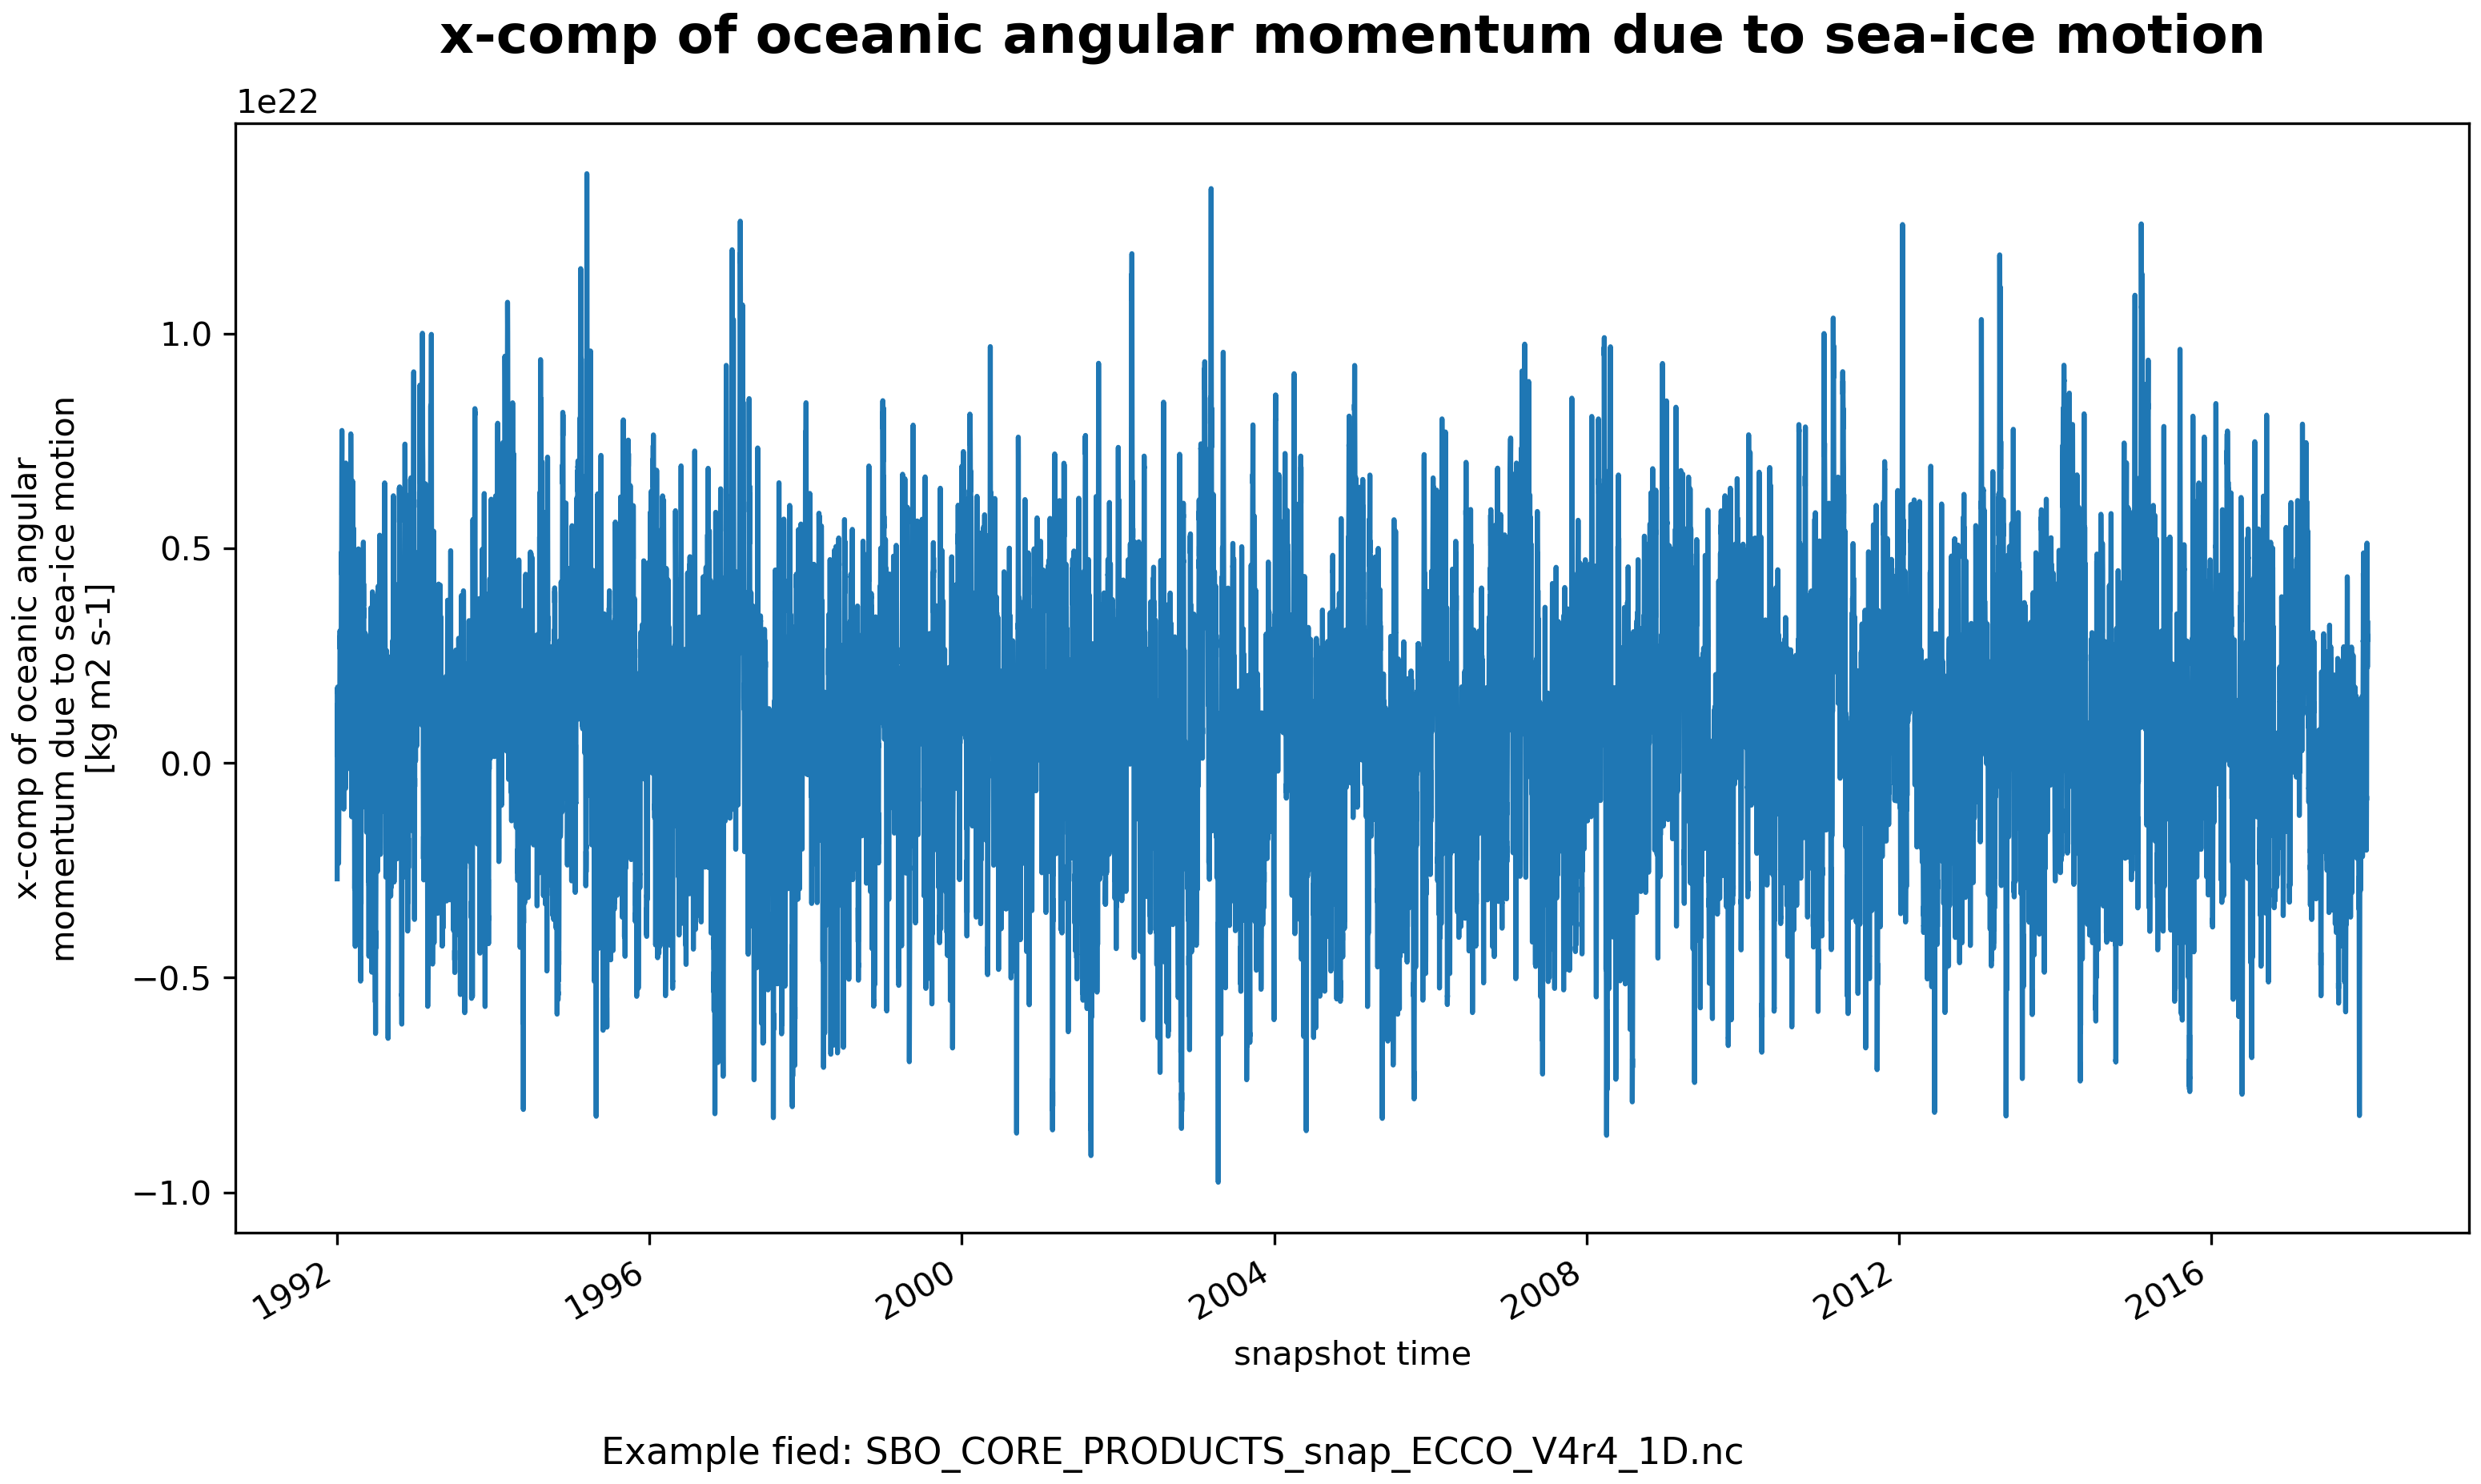
\includegraphics[scale=0.55]{../images/plots/oneD_plots/SBO_Core_Products/xoamc_si.png}
\caption{Dataset: SBO\_CORE\_PRODUCTS Variable: xoamc\_si}
\label{tab:table-SBO_CORE_PRODUCTS_xoamc_si-Plot}
\end{figure}
\pagebreak
\subsubsection{1D Variable xoamp}
\begin{longtable}{|m{0.06\textwidth}|m{0.41\textwidth}|m{0.39\textwidth}|m{0.06\textwidth}|}
\caption{CDL description of SBO\_CORE\_PRODUCTS's xoamp variable}
\label{tab:table-SBO_CORE_PRODUCTS_xoamp} \\ 
\hline \endhead \hline \endfoot
\rowcolor{lightgray} \textbf{Storage Type} & \textbf{Variable Name} & \textbf{Description} & \textbf{Unit} \\ \hline
float64 & xoamp & x-comp of oceanic angular momentum due to pressure & kg m2 s-1 \\ \hline
\rowcolor{lightgray}  \multicolumn{4}{|p{1.00\textwidth}|}{\textbf{CDL Description}} \\ \hline
\multicolumn{4}{|p{1.00\textwidth}|}{\makecell{\parbox{1\textwidth}{float64 xoamp(time)\\
\hspace*{0.5cm}xoamp: \_FillValue = 9.969209968386869e+36\\
\hspace*{0.5cm}xoamp: coverage\_content\_type = modelResult\\
\hspace*{0.5cm}xoamp: long\_name = x: comp of oceanic angular momentum due to pressure\\
\hspace*{0.5cm}xoamp: units = kg m2 s: 1\\
\hspace*{0.5cm}xoamp: valid\_min = 1.3543642768158851e+29\\
\hspace*{0.5cm}xoamp: valid\_max = 1.3546098666231897e+29\\
\hspace*{0.5cm}xoamp: coordinates = time}}} \\ \hline
\rowcolor{lightgray} \multicolumn{4}{|p{1.00\textwidth}|}{\textbf{Comments}} \\ \hline
\multicolumn{4}{|p{1\textwidth}|}{N/A} \\ \hline
\end{longtable}

\begin{figure}[H]
\centering
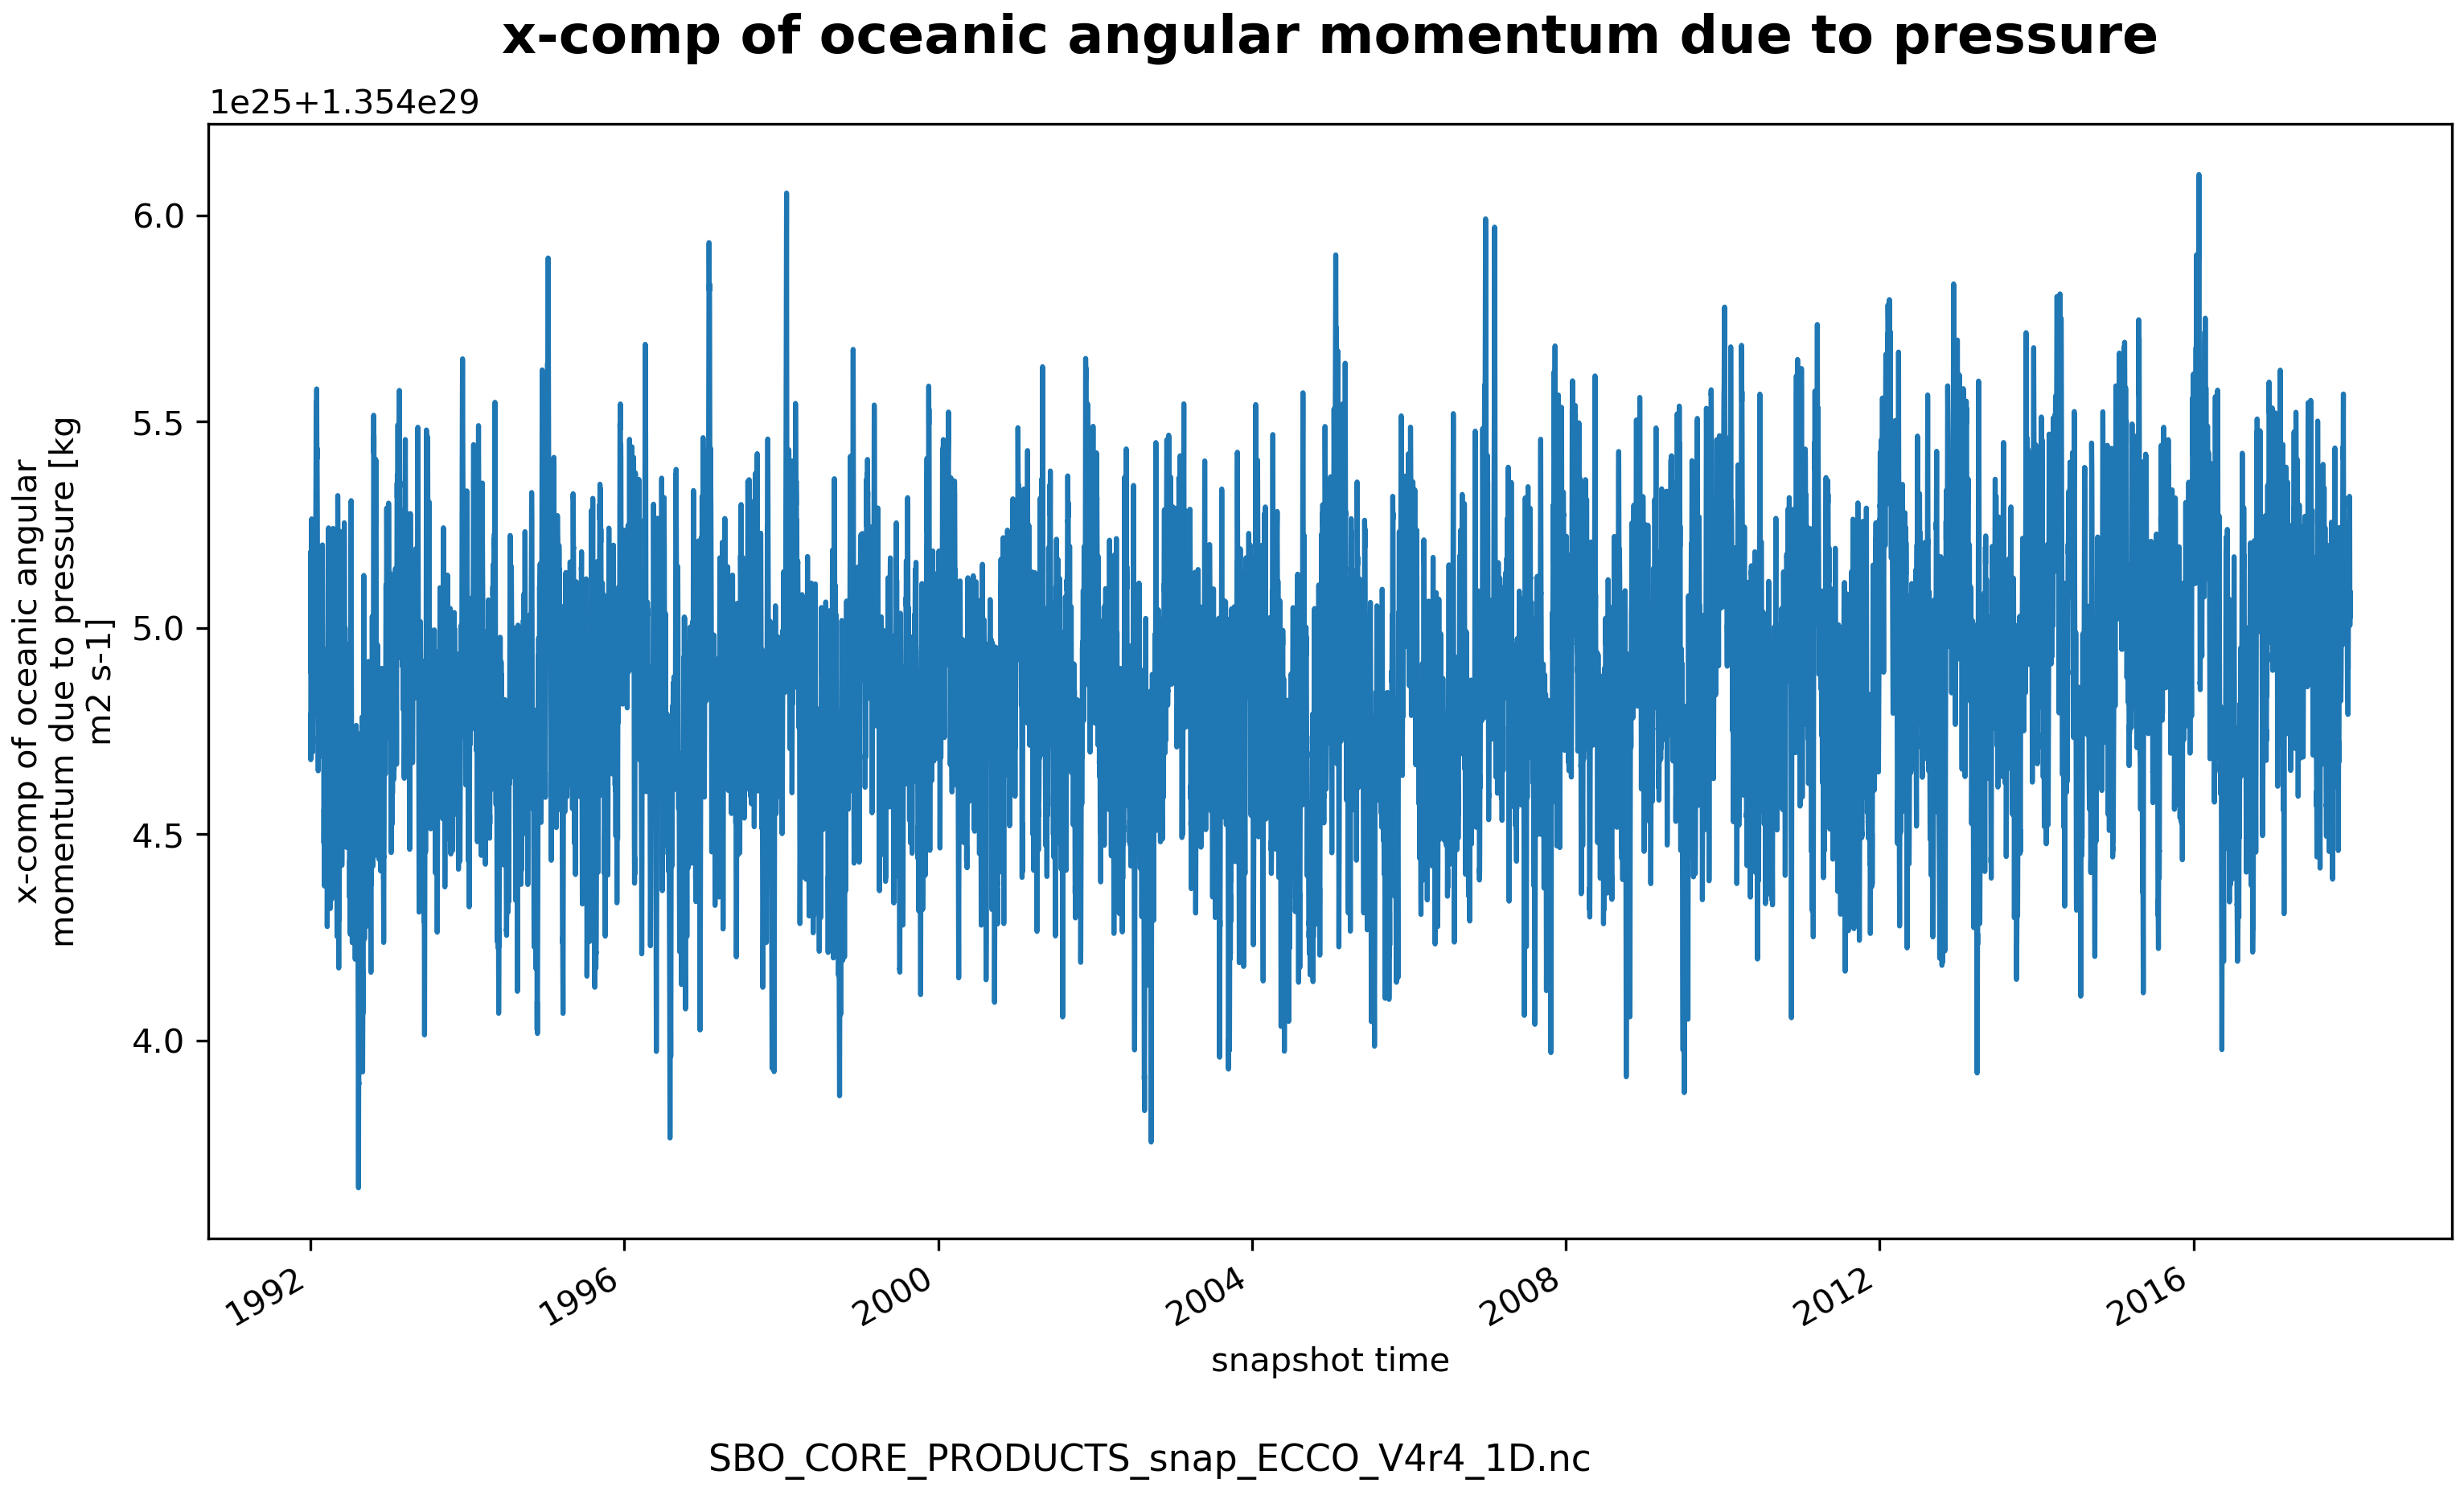
\includegraphics[scale=0.55]{../images/plots/oneD_plots/SBO_Core_Products/xoamp.png}
\caption{Dataset: SBO\_CORE\_PRODUCTS Variable: xoamp}
\label{tab:table-SBO_CORE_PRODUCTS_xoamp-Plot}
\end{figure}
\pagebreak
\subsubsection{1D Variable xoamp\_dsl}
\begin{longtable}{|m{0.06\textwidth}|m{0.41\textwidth}|m{0.39\textwidth}|m{0.06\textwidth}|}
\caption{CDL description of SBO\_CORE\_PRODUCTS's xoamp\_dsl variable}
\label{tab:table-SBO_CORE_PRODUCTS_xoamp_dsl} \\ 
\hline \endhead \hline \endfoot
\rowcolor{lightgray} \textbf{Storage Type} & \textbf{Variable Name} & \textbf{Description} & \textbf{Unit} \\ \hline
float64 & xoamp\_dsl & x-comp of oceanic angular momentum due to pressure based on dynamic (IB-corrected) sea level & kg m2 s-1 \\ \hline
\rowcolor{lightgray}  \multicolumn{4}{|p{1.00\textwidth}|}{\textbf{CDL Description}} \\ \hline
\multicolumn{4}{|p{1.00\textwidth}|}{\makecell{\parbox{1\textwidth}{float64 xoamp\_dsl(time)\\
\hspace*{0.5cm}xoamp\_dsl: \_FillValue = 9.969209968386869e+36\\
\hspace*{0.5cm}xoamp\_dsl: coverage\_content\_type = modelResult\\
\hspace*{0.5cm}xoamp\_dsl: long\_name = x: comp of oceanic angular momentum due to pressure based on dynamic (IB: corrected) sea level\\
\hspace*{0.5cm}xoamp\_dsl: units = kg m2 s: 1\\
\hspace*{0.5cm}xoamp\_dsl: valid\_min = 1.354440386439953e+29\\
\hspace*{0.5cm}xoamp\_dsl: valid\_max = 1.3545518352698056e+29\\
\hspace*{0.5cm}xoamp\_dsl: coordinates = time}}} \\ \hline
\rowcolor{lightgray} \multicolumn{4}{|p{1.00\textwidth}|}{\textbf{Comments}} \\ \hline
\multicolumn{4}{|p{1\textwidth}|}{N/A} \\ \hline
\end{longtable}

\begin{figure}[H]
\centering
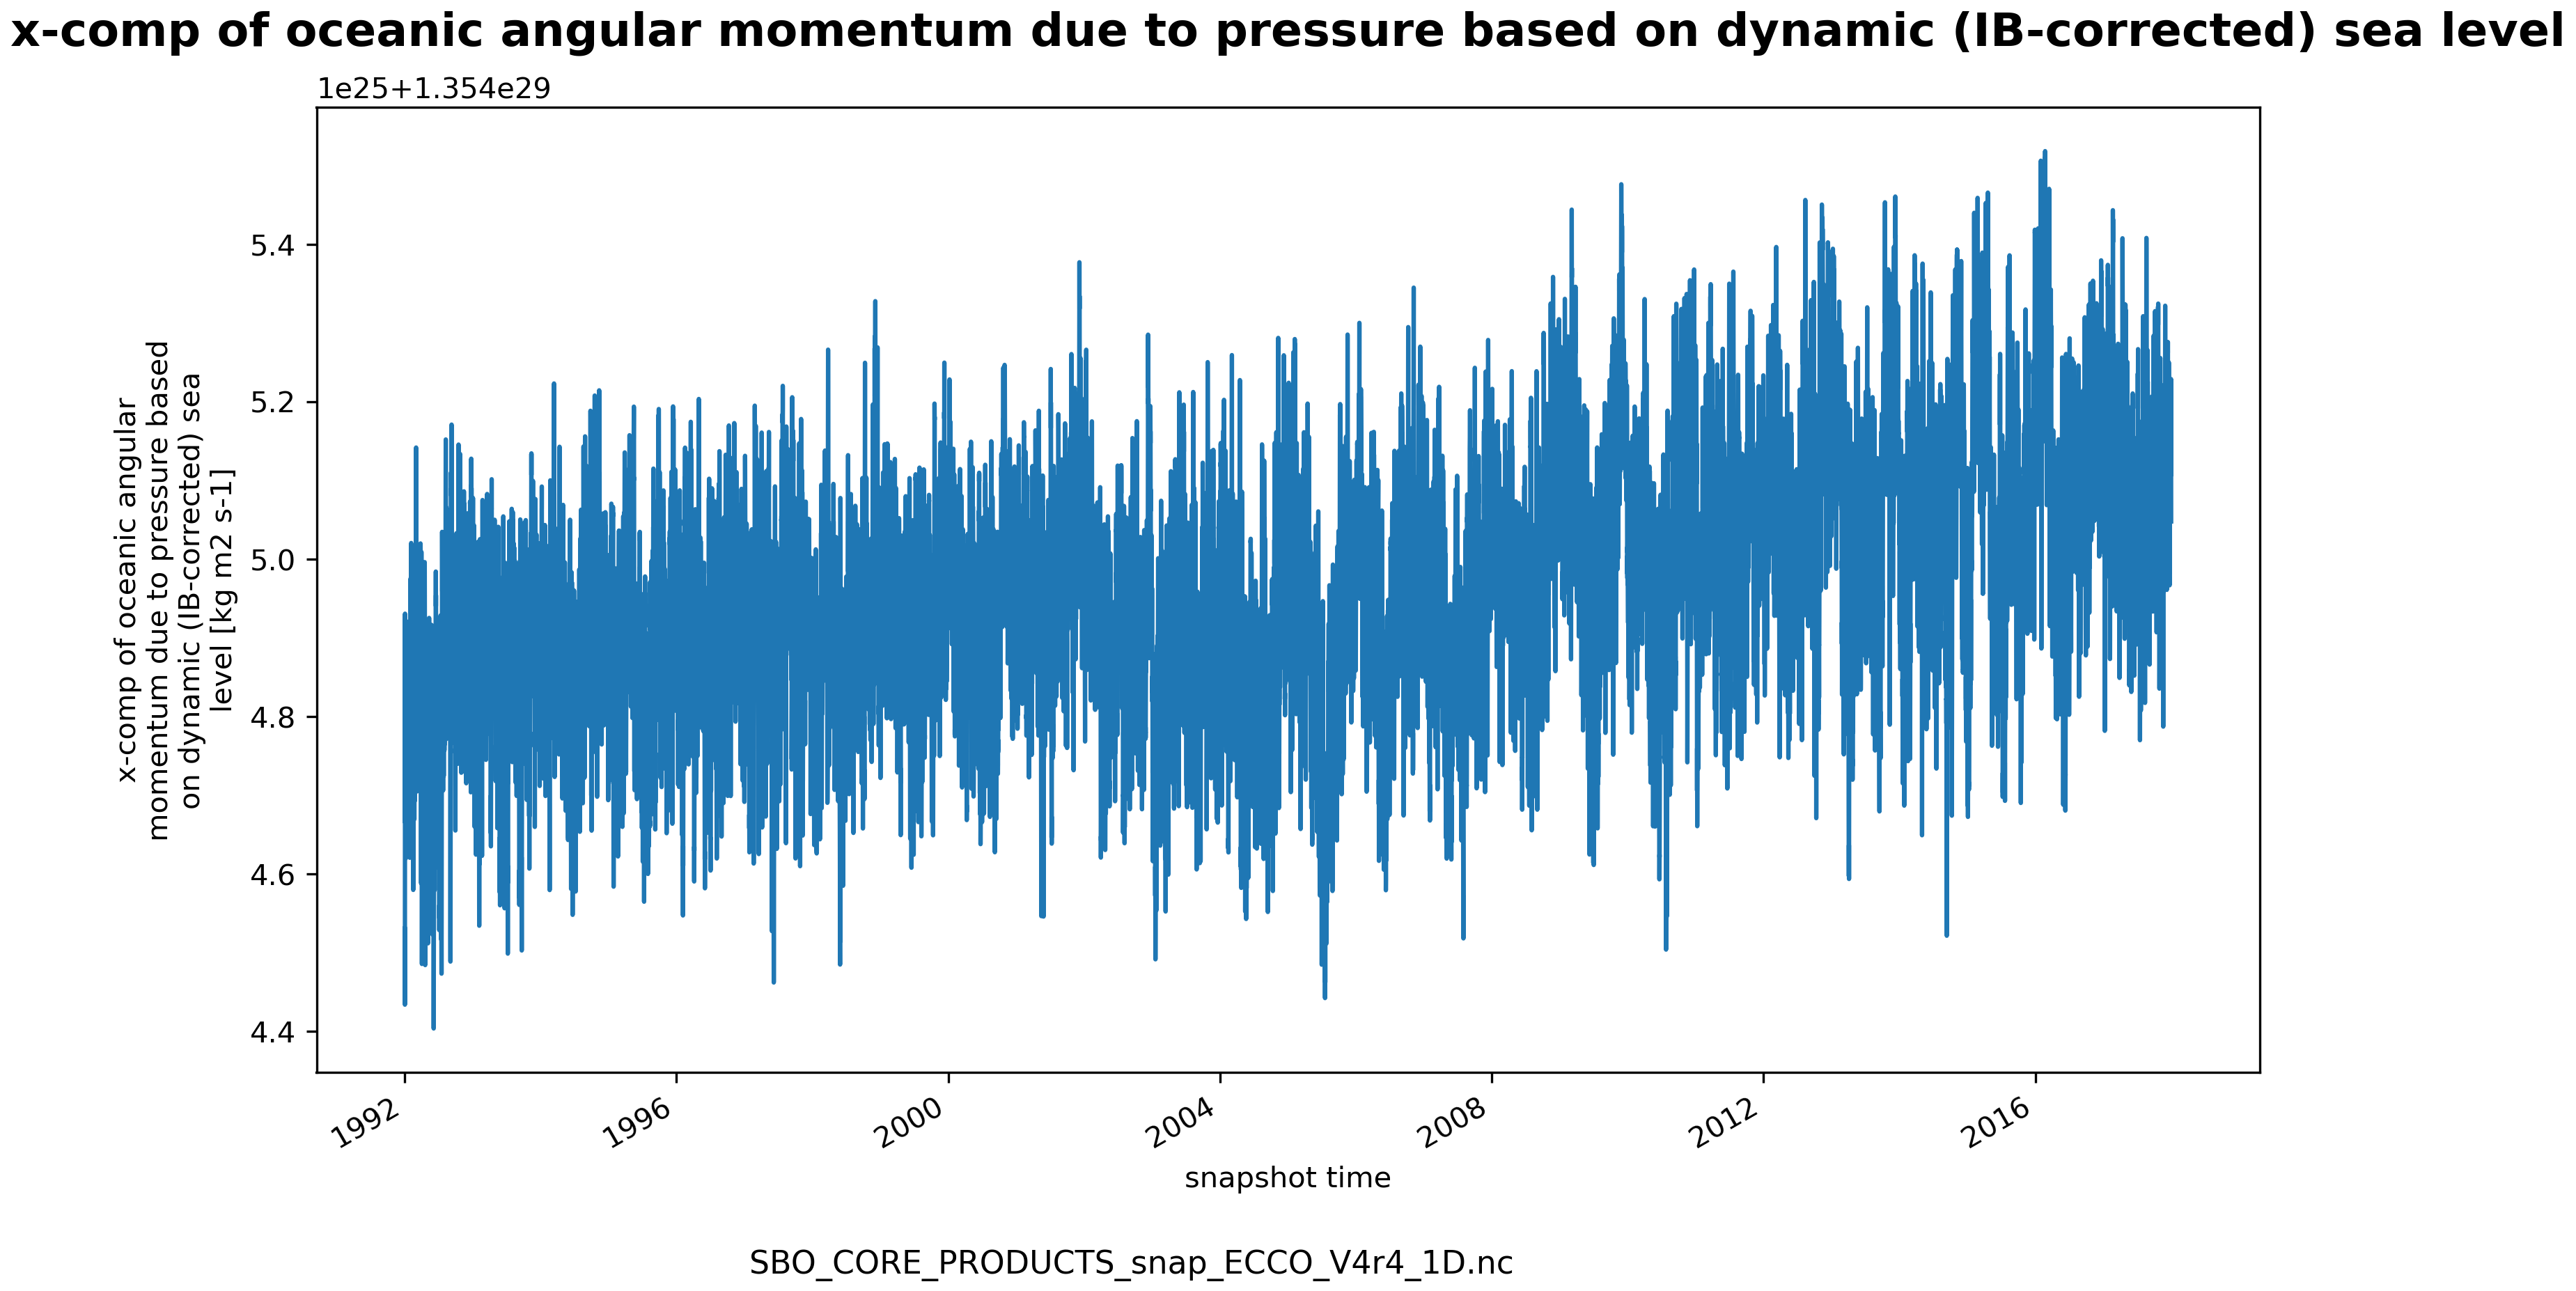
\includegraphics[scale=0.55]{../images/plots/oneD_plots/SBO_Core_Products/xoamp_dsl.png}
\caption{Dataset: SBO\_CORE\_PRODUCTS Variable: xoamp\_dsl}
\label{tab:table-SBO_CORE_PRODUCTS_xoamp_dsl-Plot}
\end{figure}
\pagebreak
\subsubsection{1D Variable xoamp\_fw}
\begin{longtable}{|m{0.06\textwidth}|m{0.41\textwidth}|m{0.39\textwidth}|m{0.06\textwidth}|}
\caption{CDL description of SBO\_CORE\_PRODUCTS's xoamp\_fw variable}
\label{tab:table-SBO_CORE_PRODUCTS_xoamp_fw} \\ 
\hline \endhead \hline \endfoot
\rowcolor{lightgray} \textbf{Storage Type} & \textbf{Variable Name} & \textbf{Description} & \textbf{Unit} \\ \hline
float64 & xoamp\_fw & x-comp of oceanic angular momentum due to freshwater flux & kg m2 s-1 \\ \hline
\rowcolor{lightgray}  \multicolumn{4}{|p{1.00\textwidth}|}{\textbf{CDL Description}} \\ \hline
\multicolumn{4}{|p{1.00\textwidth}|}{\makecell{\parbox{1\textwidth}{float64 xoamp\_fw(time)\\
\hspace*{0.5cm}xoamp\_fw: \_FillValue = 9.969209968386869e+36\\
\hspace*{0.5cm}xoamp\_fw: coverage\_content\_type = modelResult\\
\hspace*{0.5cm}xoamp\_fw: long\_name = x: comp of oceanic angular momentum due to freshwater flux\\
\hspace*{0.5cm}xoamp\_fw: units = kg m2 s: 1\\
\hspace*{0.5cm}xoamp\_fw: valid\_min = 1.805799644912138e+24\\
\hspace*{0.5cm}xoamp\_fw: valid\_max = 3.351358892803656e+24\\
\hspace*{0.5cm}xoamp\_fw: coordinates = time}}} \\ \hline
\rowcolor{lightgray} \multicolumn{4}{|p{1.00\textwidth}|}{\textbf{Comments}} \\ \hline
\multicolumn{4}{|p{1\textwidth}|}{N/A} \\ \hline
\end{longtable}

\begin{figure}[H]
\centering
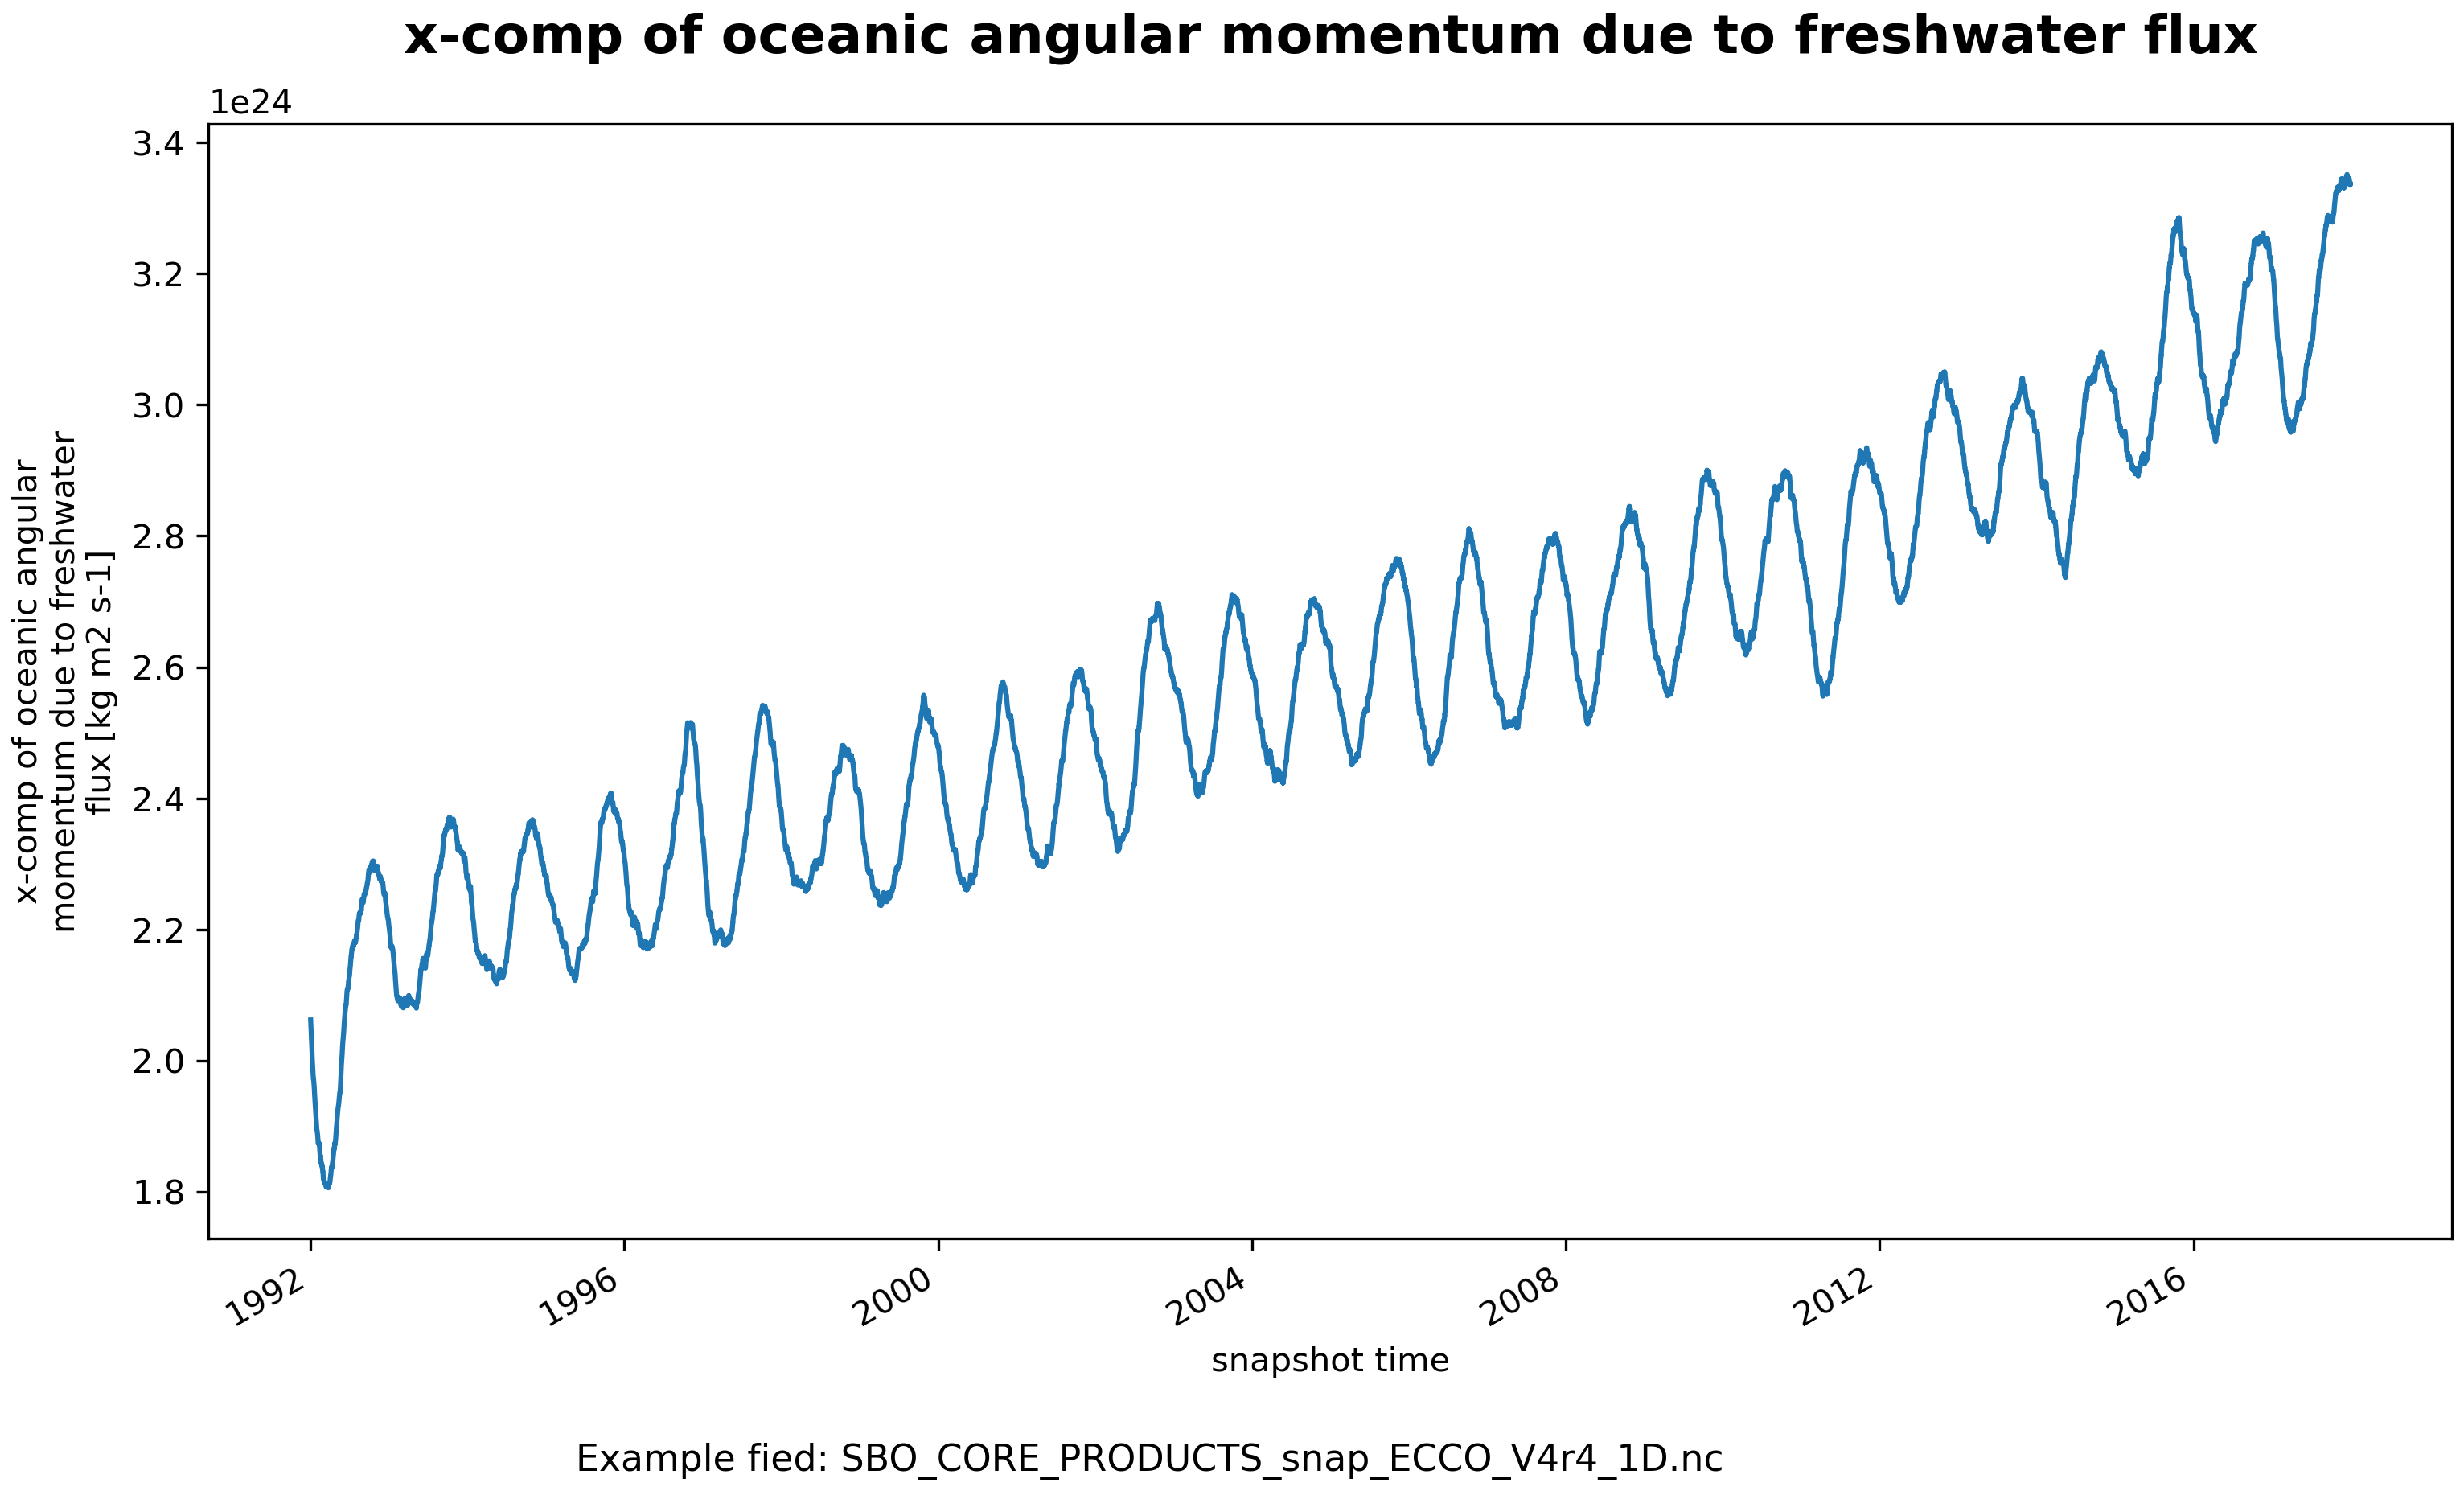
\includegraphics[scale=0.55]{../images/plots/oneD_plots/SBO_Core_Products/xoamp_fw.png}
\caption{Dataset: SBO\_CORE\_PRODUCTS Variable: xoamp\_fw}
\label{tab:table-SBO_CORE_PRODUCTS_xoamp_fw-Plot}
\end{figure}
\pagebreak
\subsubsection{1D Variable ycom}
\begin{longtable}{|m{0.06\textwidth}|m{0.41\textwidth}|m{0.39\textwidth}|m{0.06\textwidth}|}
\caption{CDL description of SBO\_CORE\_PRODUCTS's ycom variable}
\label{tab:table-SBO_CORE_PRODUCTS_ycom} \\ 
\hline \endhead \hline \endfoot
\rowcolor{lightgray} \textbf{Storage Type} & \textbf{Variable Name} & \textbf{Description} & \textbf{Unit} \\ \hline
float64 & ycom & y-comp of center-of-mass of ocean & m \\ \hline
\rowcolor{lightgray}  \multicolumn{4}{|p{1.00\textwidth}|}{\textbf{CDL Description}} \\ \hline
\multicolumn{4}{|p{1.00\textwidth}|}{\makecell{\parbox{1\textwidth}{float64 ycom(time)\\
\hspace*{0.5cm}ycom: \_FillValue = 9.969209968386869e+36\\
\hspace*{0.5cm}ycom: coverage\_content\_type = modelResult\\
\hspace*{0.5cm}ycom: long\_name = y: comp of center: of: mass of ocean\\
\hspace*{0.5cm}ycom: units = m\\
\hspace*{0.5cm}ycom: valid\_min = : 466387.24450374383\\
\hspace*{0.5cm}ycom: valid\_max = : 466327.21844756586\\
\hspace*{0.5cm}ycom: coordinates = time}}} \\ \hline
\rowcolor{lightgray} \multicolumn{4}{|p{1.00\textwidth}|}{\textbf{Comments}} \\ \hline
\multicolumn{4}{|p{1\textwidth}|}{N/A} \\ \hline
\end{longtable}

\begin{figure}[H]
\centering
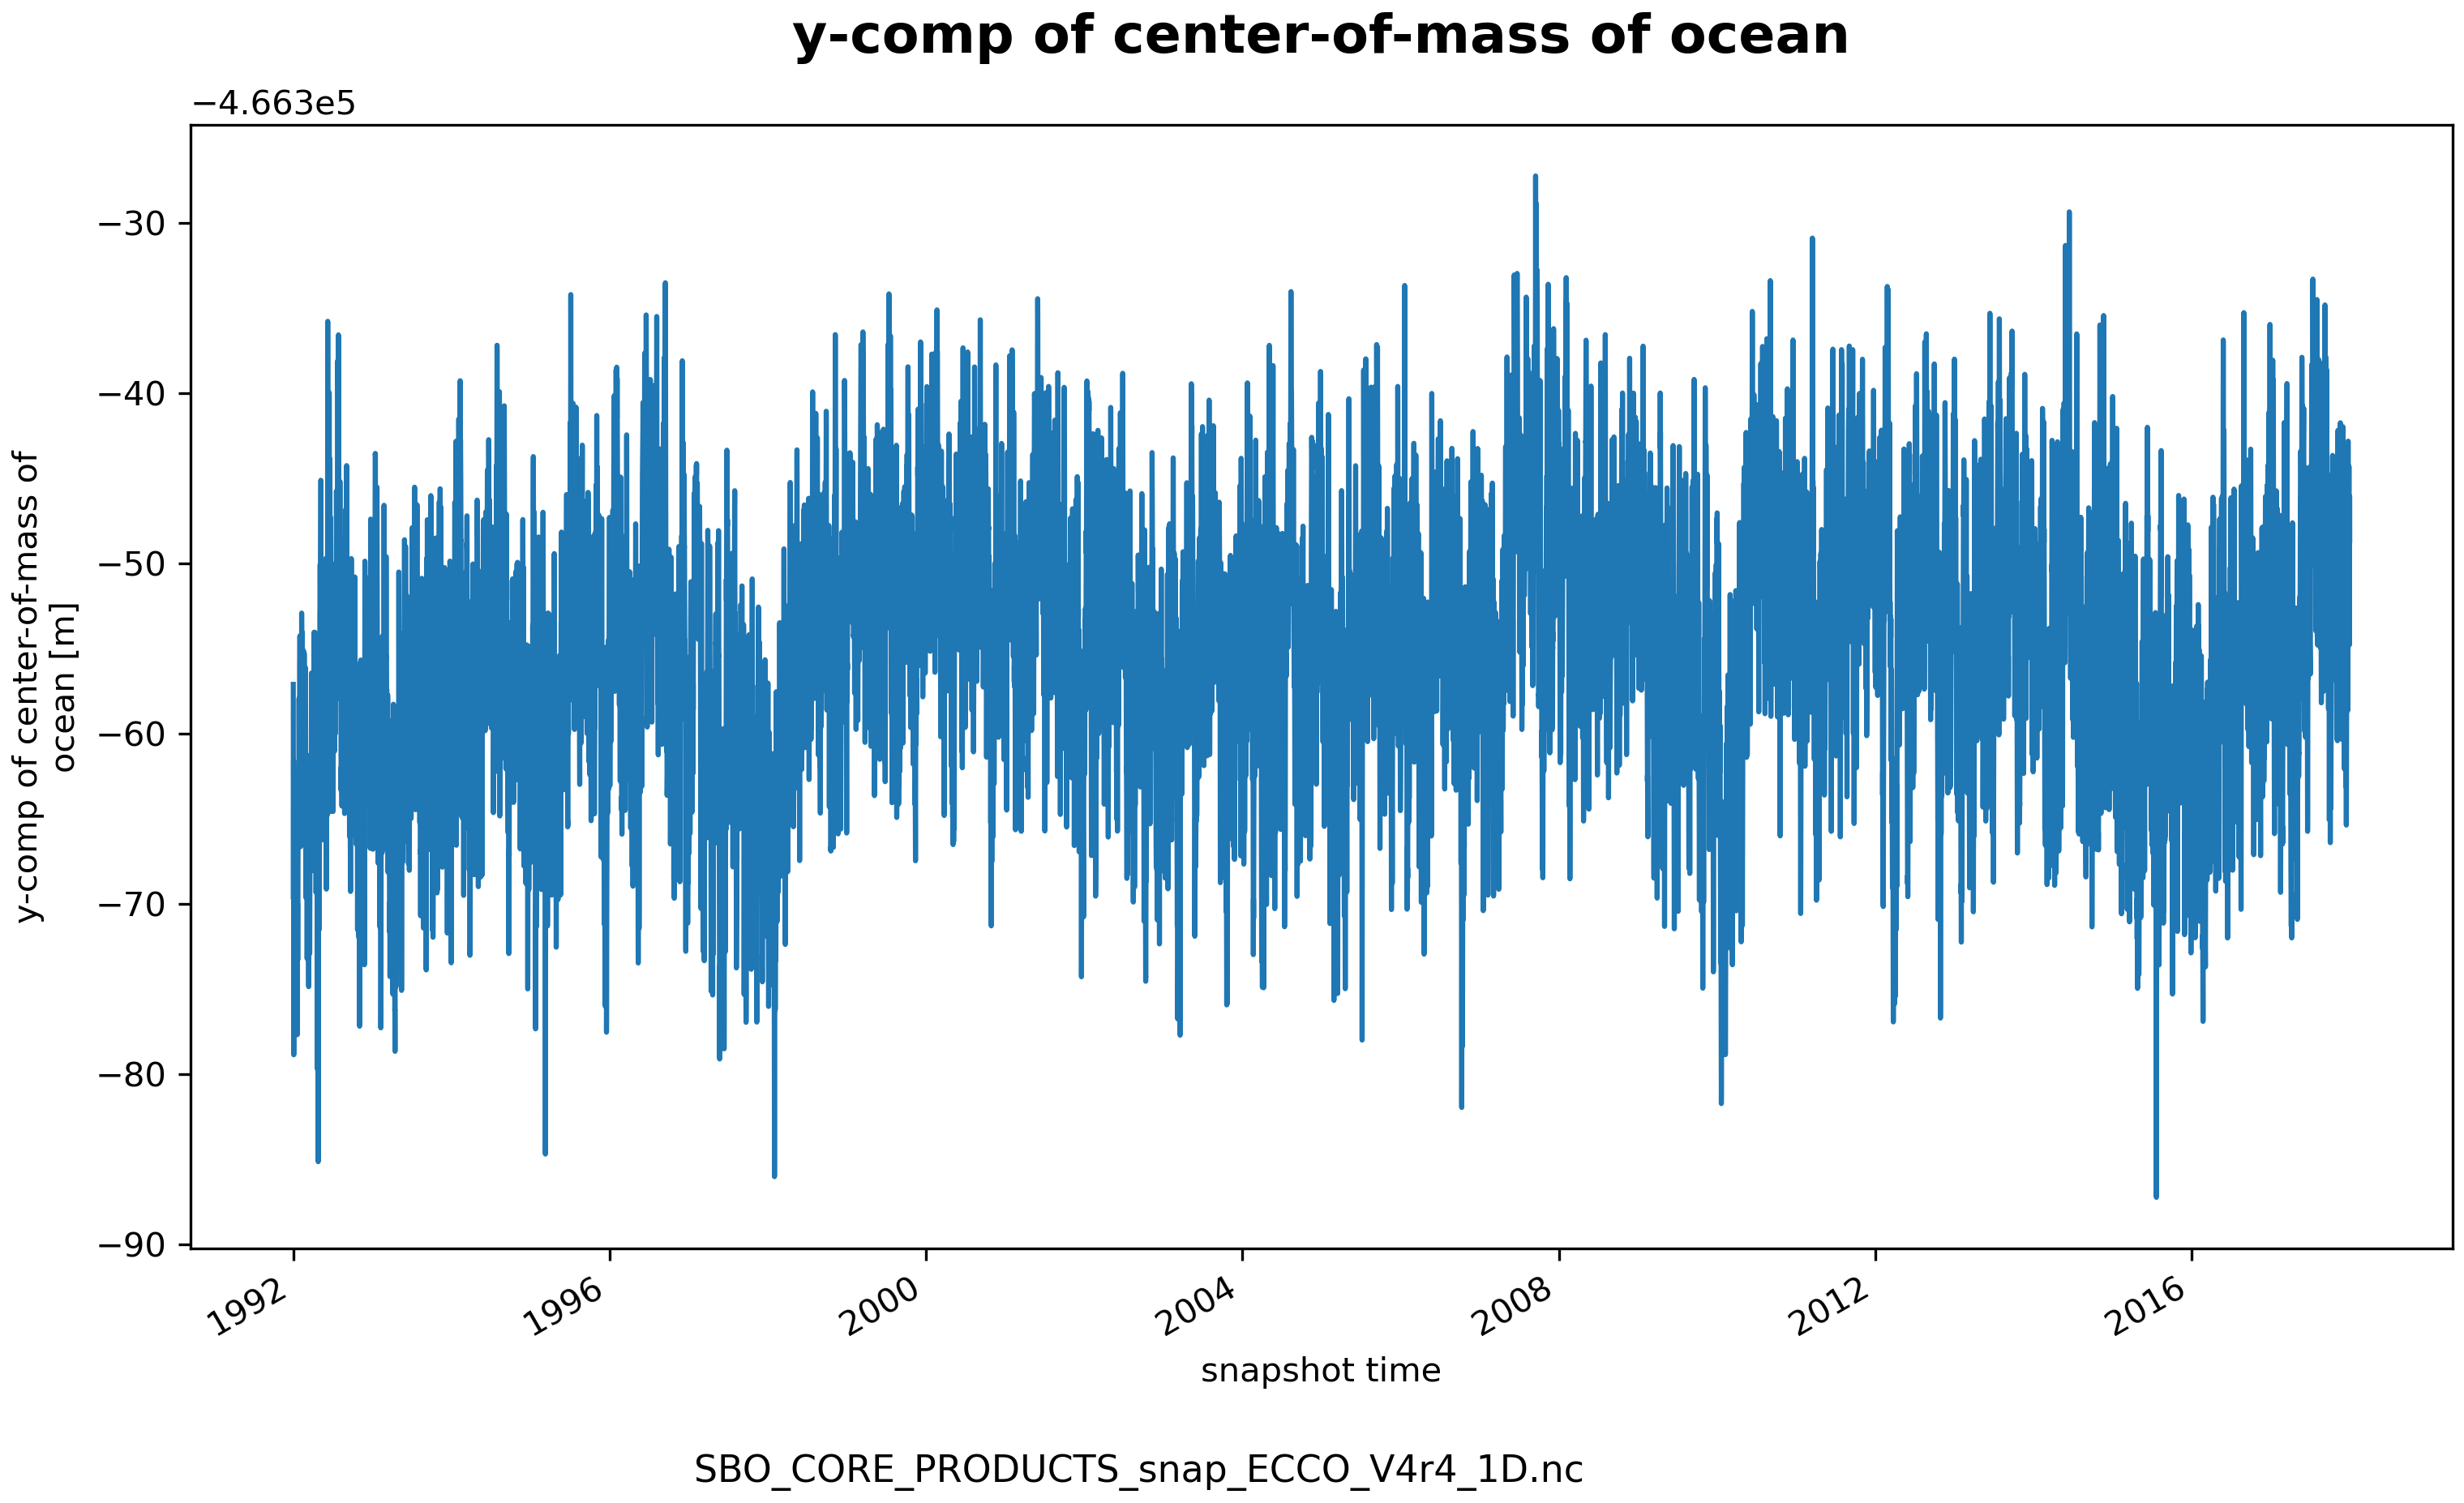
\includegraphics[scale=0.55]{../images/plots/oneD_plots/SBO_Core_Products/ycom.png}
\caption{Dataset: SBO\_CORE\_PRODUCTS Variable: ycom}
\label{tab:table-SBO_CORE_PRODUCTS_ycom-Plot}
\end{figure}
\pagebreak
\subsubsection{1D Variable ycom\_fw}
\begin{longtable}{|m{0.06\textwidth}|m{0.41\textwidth}|m{0.39\textwidth}|m{0.06\textwidth}|}
\caption{CDL description of SBO\_CORE\_PRODUCTS's ycom\_fw variable}
\label{tab:table-SBO_CORE_PRODUCTS_ycom_fw} \\ 
\hline \endhead \hline \endfoot
\rowcolor{lightgray} \textbf{Storage Type} & \textbf{Variable Name} & \textbf{Description} & \textbf{Unit} \\ \hline
float64 & ycom\_fw & y-comp of center-of-mass of freshwater flux & m \\ \hline
\rowcolor{lightgray}  \multicolumn{4}{|p{1.00\textwidth}|}{\textbf{CDL Description}} \\ \hline
\multicolumn{4}{|p{1.00\textwidth}|}{\makecell{\parbox{1\textwidth}{float64 ycom\_fw(time)\\
\hspace*{0.5cm}ycom\_fw: \_FillValue = 9.969209968386869e+36\\
\hspace*{0.5cm}ycom\_fw: coverage\_content\_type = modelResult\\
\hspace*{0.5cm}ycom\_fw: long\_name = y: comp of center: of: mass of freshwater flux\\
\hspace*{0.5cm}ycom\_fw: units = m\\
\hspace*{0.5cm}ycom\_fw: valid\_min = : 324750.41529212013\\
\hspace*{0.5cm}ycom\_fw: valid\_max = : 324750.4152921157\\
\hspace*{0.5cm}ycom\_fw: coordinates = time}}} \\ \hline
\rowcolor{lightgray} \multicolumn{4}{|p{1.00\textwidth}|}{\textbf{Comments}} \\ \hline
\multicolumn{4}{|p{1\textwidth}|}{N/A} \\ \hline
\end{longtable}

\begin{figure}[H]
\centering
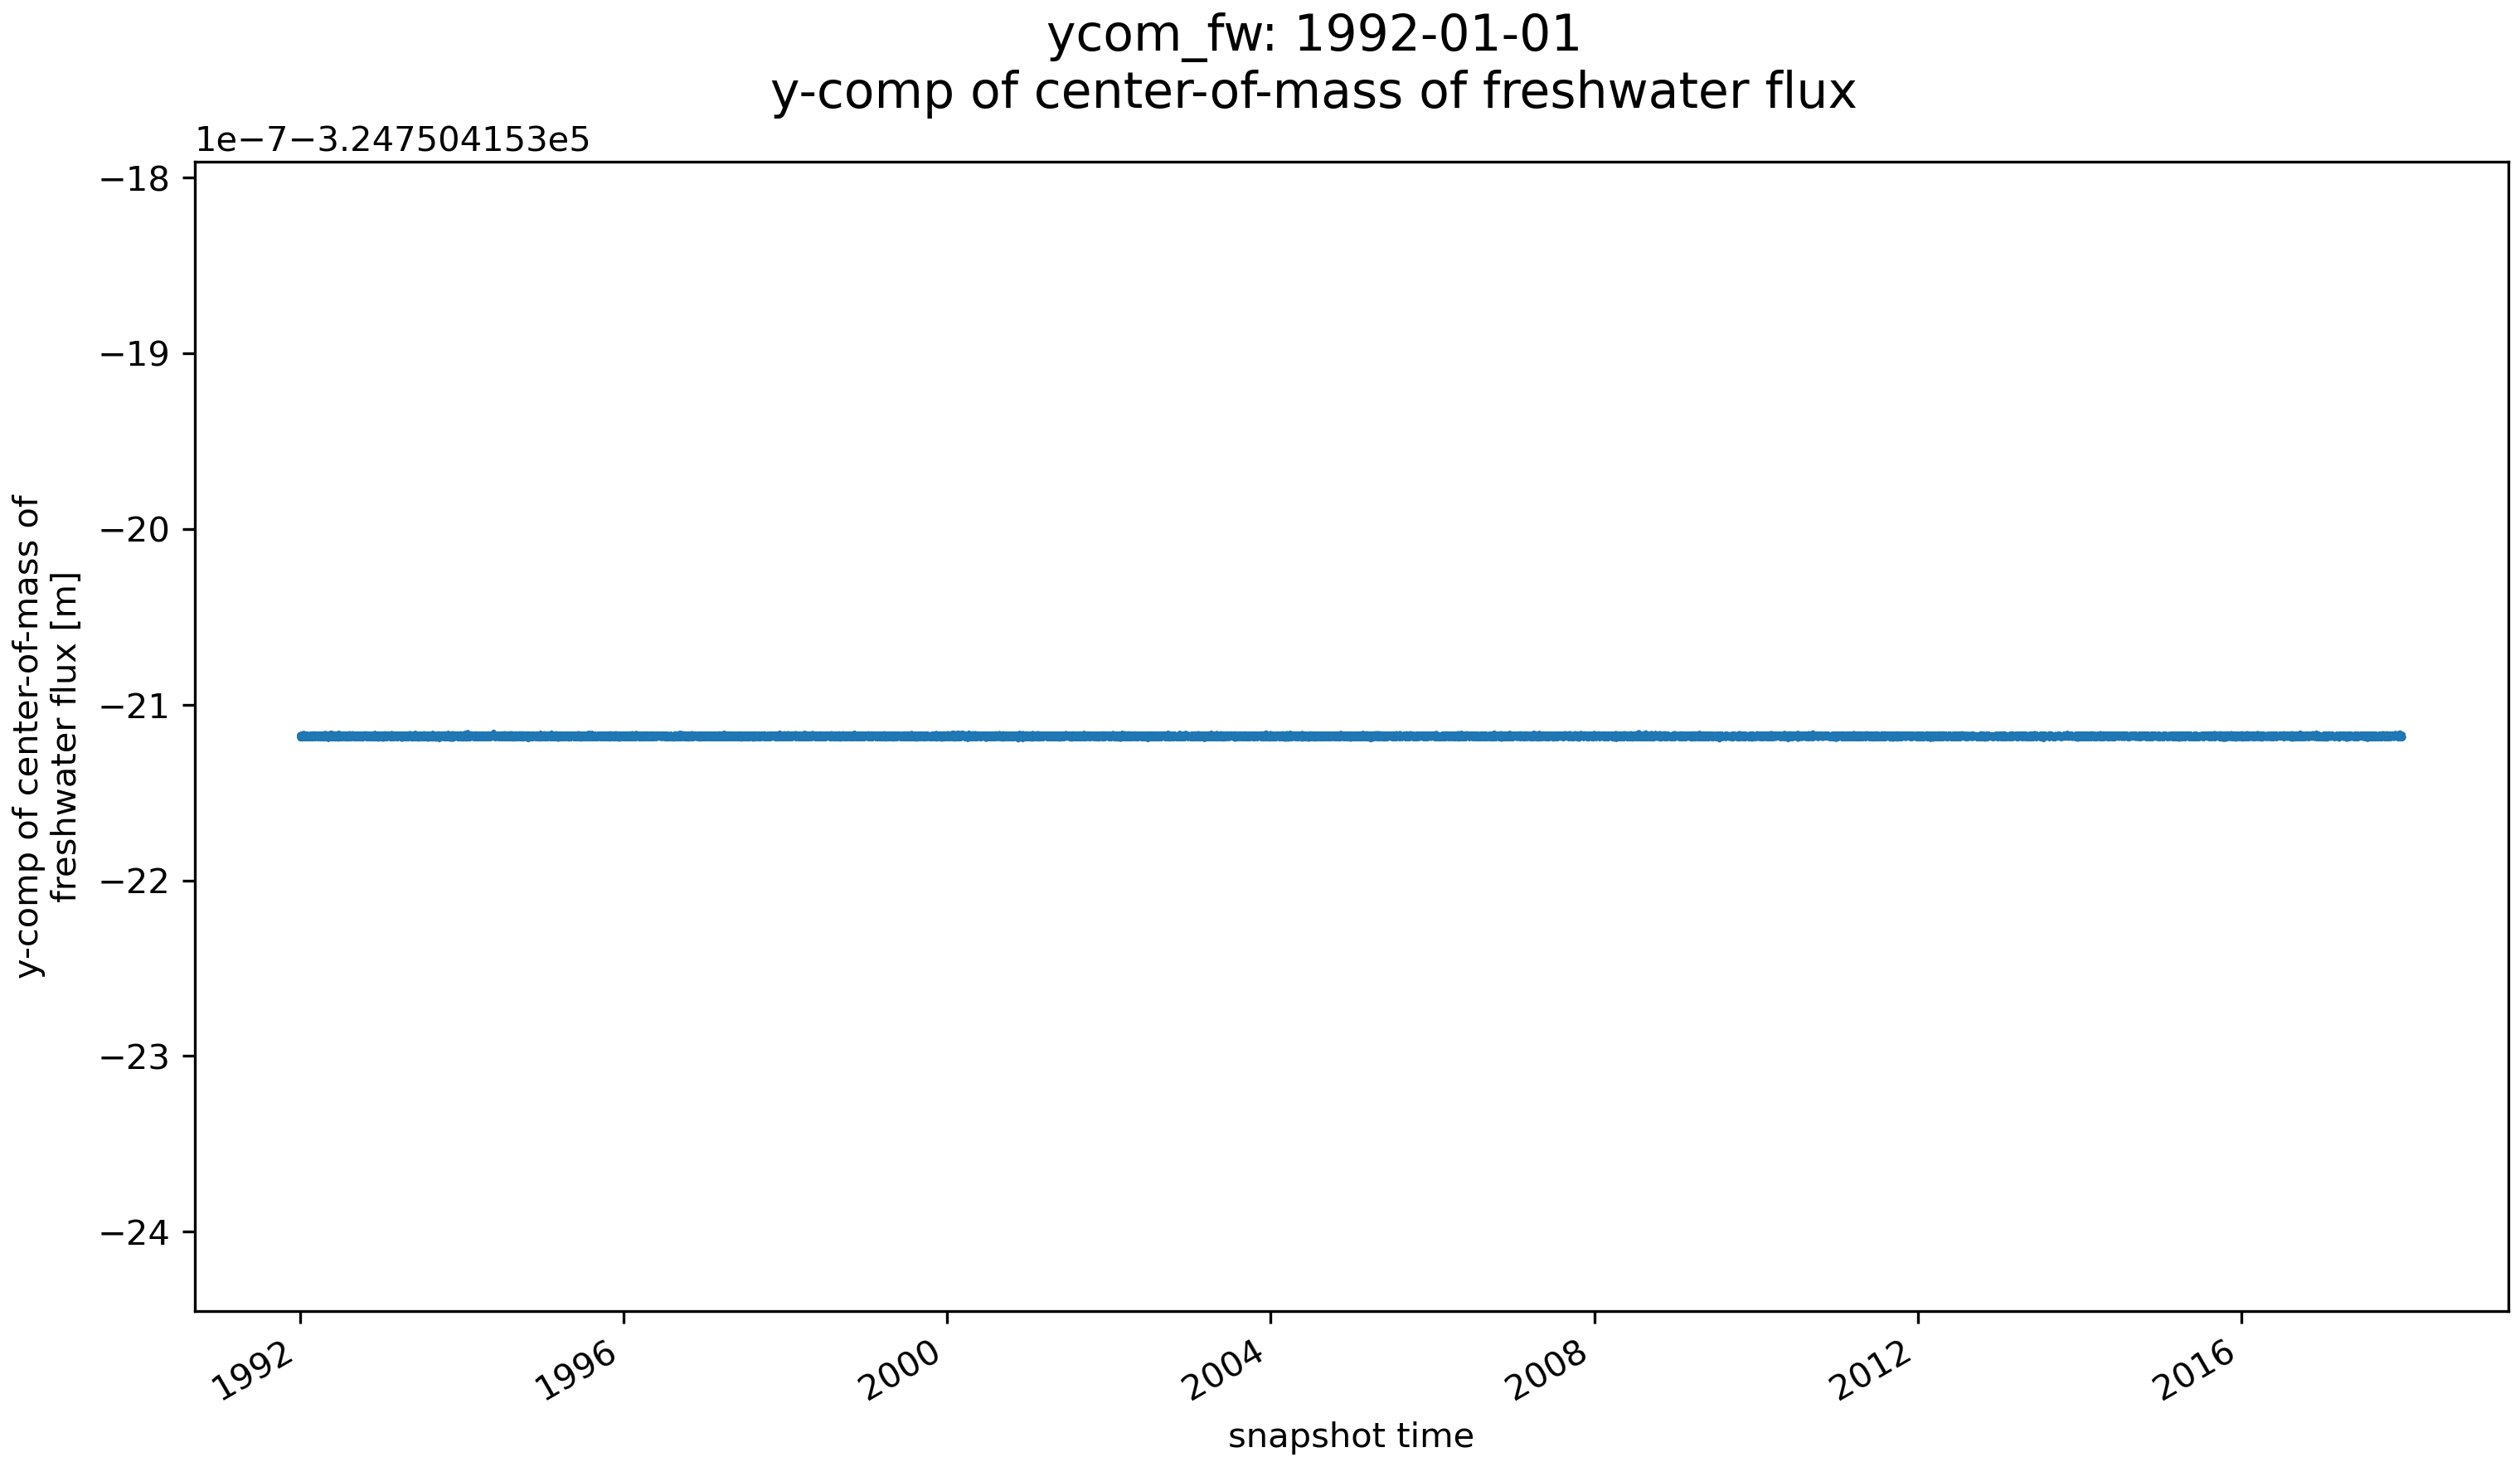
\includegraphics[scale=0.55]{../images/plots/oneD_plots/SBO_Core_Products/ycom_fw.png}
\caption{Dataset: SBO\_CORE\_PRODUCTS Variable: ycom\_fw}
\label{tab:table-SBO_CORE_PRODUCTS_ycom_fw-Plot}
\end{figure}
\pagebreak
\subsubsection{1D Variable yoamc}
\begin{longtable}{|m{0.06\textwidth}|m{0.41\textwidth}|m{0.39\textwidth}|m{0.06\textwidth}|}
\caption{CDL description of SBO\_CORE\_PRODUCTS's yoamc variable}
\label{tab:table-SBO_CORE_PRODUCTS_yoamc} \\ 
\hline \endhead \hline \endfoot
\rowcolor{lightgray} \textbf{Storage Type} & \textbf{Variable Name} & \textbf{Description} & \textbf{Unit} \\ \hline
float64 & yoamc & y-comp of oceanic angular momentum due to currents & kg m2 s-1 \\ \hline
\rowcolor{lightgray}  \multicolumn{4}{|p{1.00\textwidth}|}{\textbf{CDL Description}} \\ \hline
\multicolumn{4}{|p{1.00\textwidth}|}{\makecell{\parbox{1\textwidth}{float64 yoamc(time)\\
\hspace*{0.5cm}yoamc: \_FillValue = 9.969209968386869e+36\\
\hspace*{0.5cm}yoamc: coverage\_content\_type = modelResult\\
\hspace*{0.5cm}yoamc: long\_name = y: comp of oceanic angular momentum due to currents\\
\hspace*{0.5cm}yoamc: units = kg m2 s: 1\\
\hspace*{0.5cm}yoamc: valid\_min = : 2.19249690136359e+24\\
\hspace*{0.5cm}yoamc: valid\_max = 4.179441018940977e+24\\
\hspace*{0.5cm}yoamc: coordinates = time}}} \\ \hline
\rowcolor{lightgray} \multicolumn{4}{|p{1.00\textwidth}|}{\textbf{Comments}} \\ \hline
\multicolumn{4}{|p{1\textwidth}|}{N/A} \\ \hline
\end{longtable}

\begin{figure}[H]
\centering
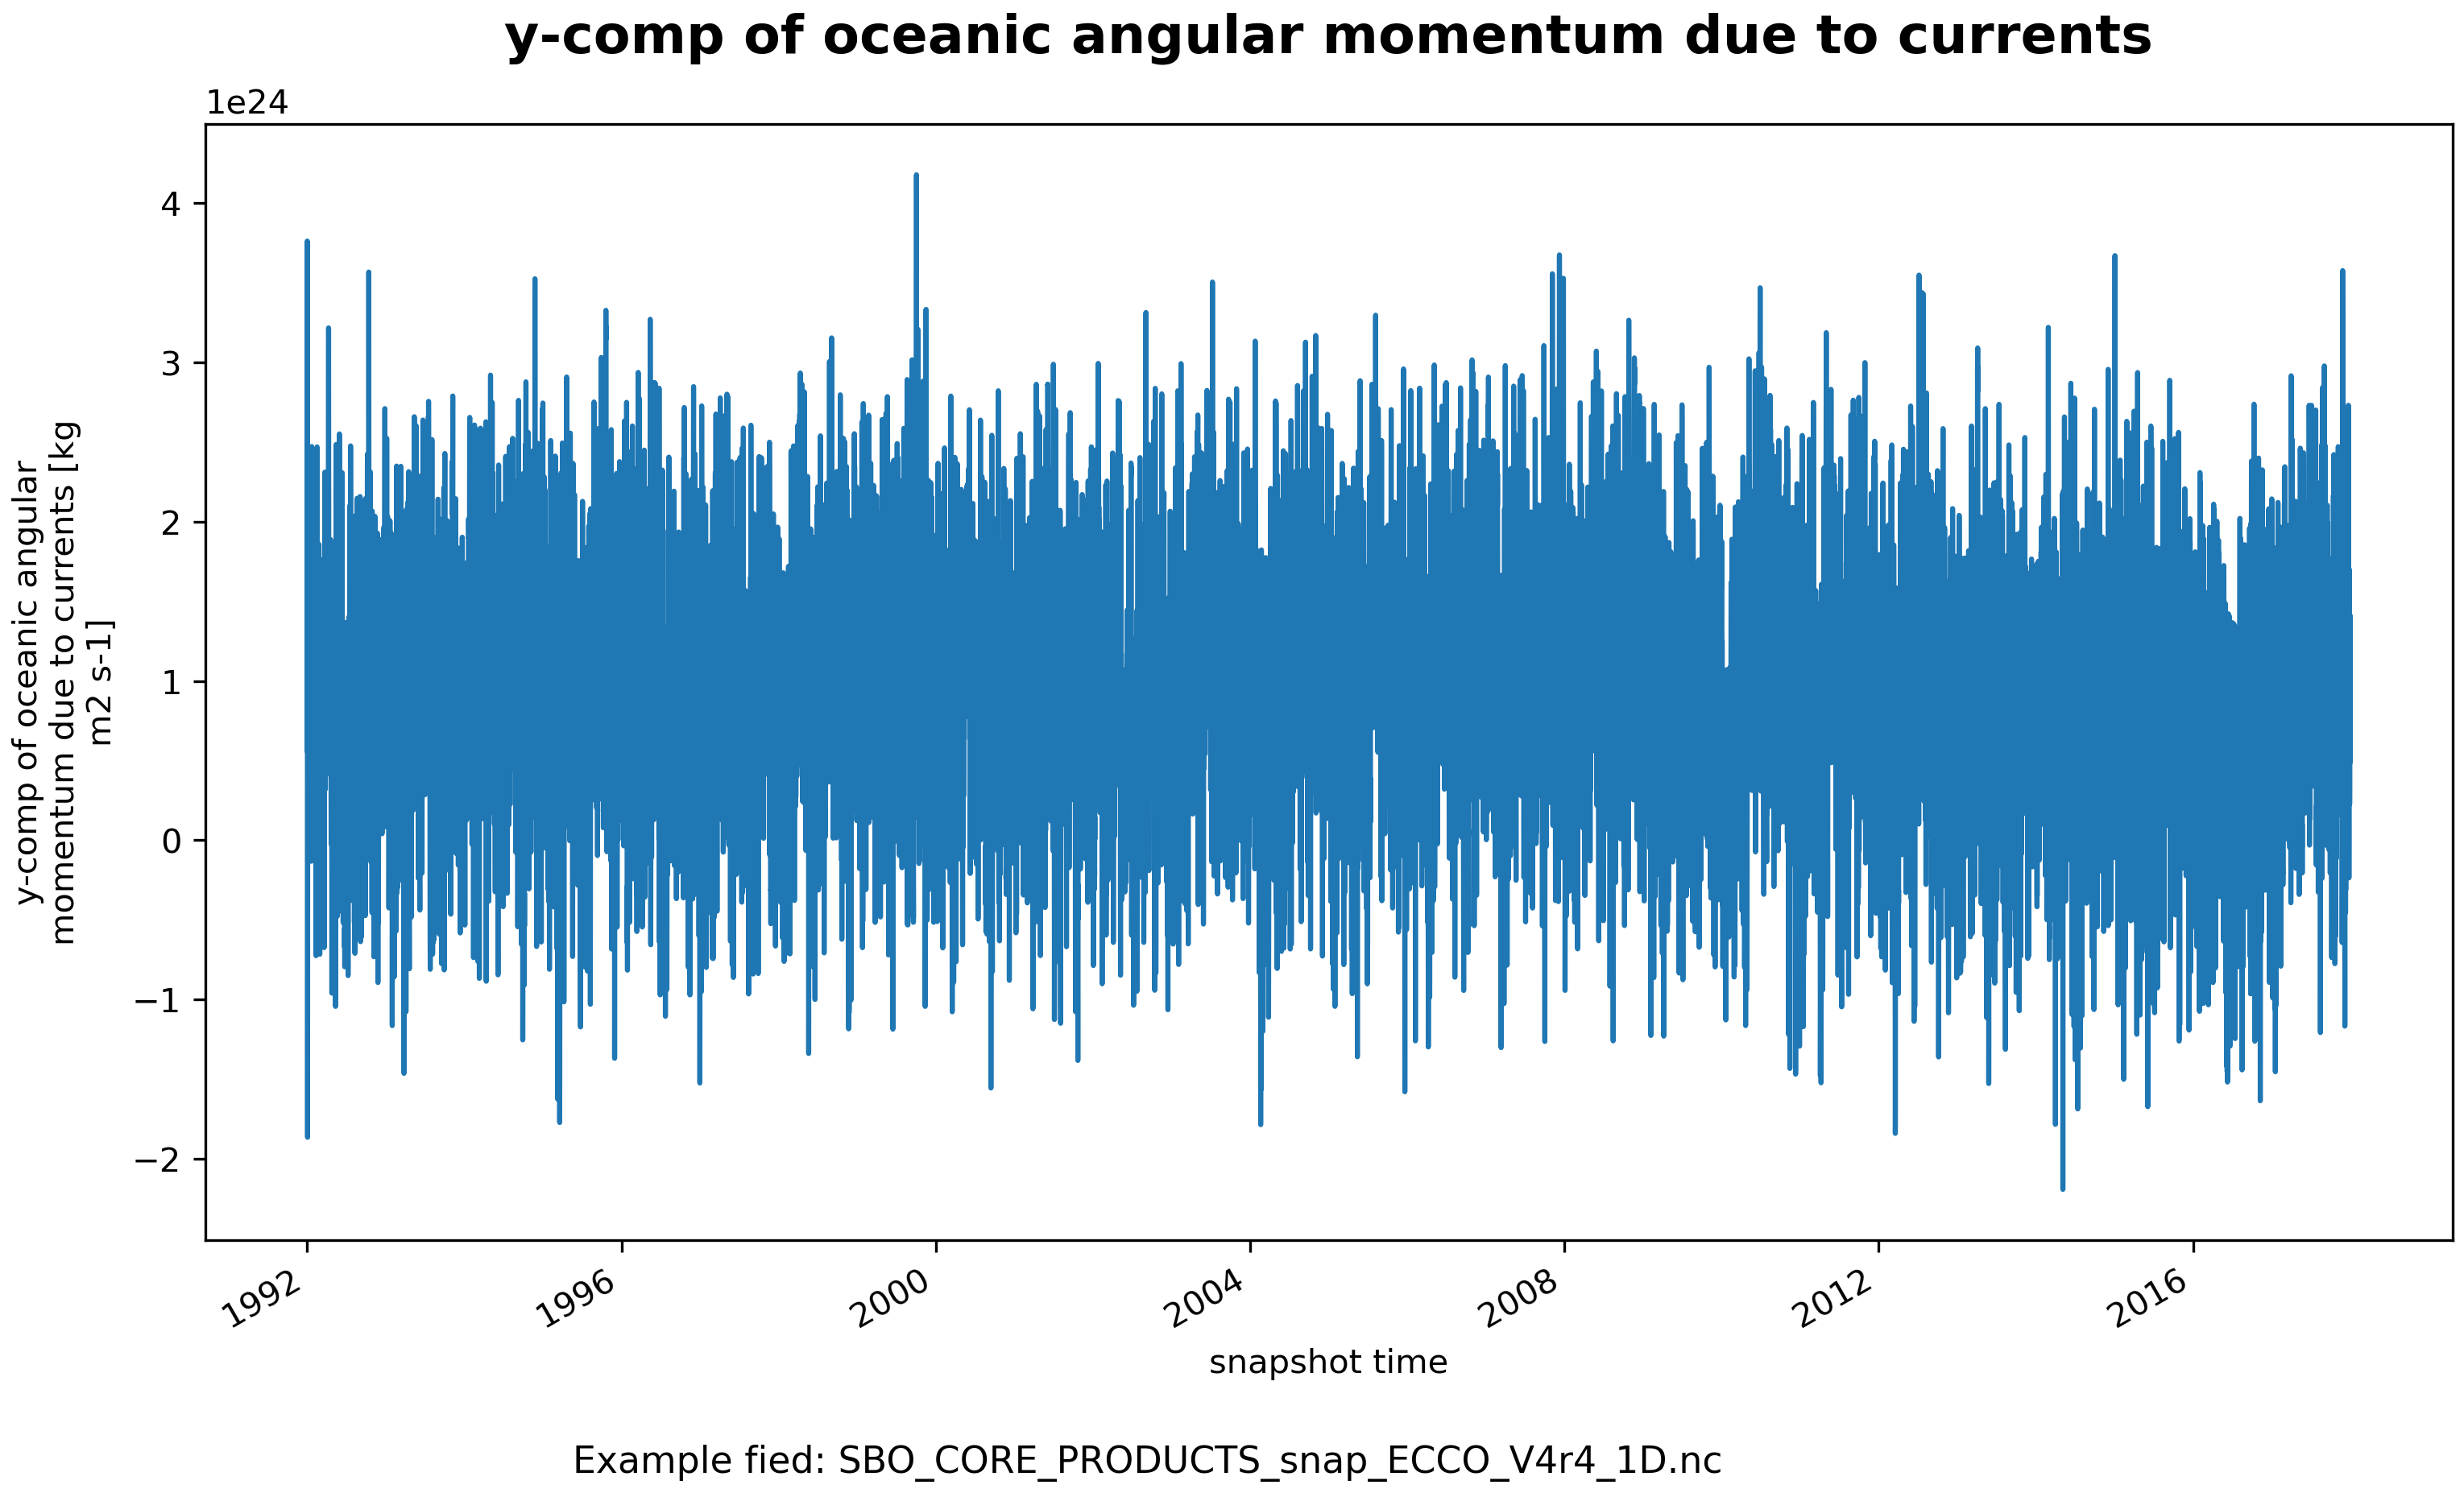
\includegraphics[scale=0.55]{../images/plots/oneD_plots/SBO_Core_Products/yoamc.png}
\caption{Dataset: SBO\_CORE\_PRODUCTS Variable: yoamc}
\label{tab:table-SBO_CORE_PRODUCTS_yoamc-Plot}
\end{figure}
\pagebreak
\subsubsection{1D Variable yoamc\_si}
\begin{longtable}{|m{0.06\textwidth}|m{0.41\textwidth}|m{0.39\textwidth}|m{0.06\textwidth}|}
\caption{CDL description of SBO\_CORE\_PRODUCTS's yoamc\_si variable}
\label{tab:table-SBO_CORE_PRODUCTS_yoamc_si} \\ 
\hline \endhead \hline \endfoot
\rowcolor{lightgray} \textbf{Storage Type} & \textbf{Variable Name} & \textbf{Description} & \textbf{Unit} \\ \hline
float64 & yoamc\_si & y-comp of oceanic angular momentum due to sea-ice motion & kg m2 s-1 \\ \hline
\rowcolor{lightgray}  \multicolumn{4}{|p{1.00\textwidth}|}{\textbf{CDL Description}} \\ \hline
\multicolumn{4}{|p{1.00\textwidth}|}{\makecell{\parbox{1\textwidth}{float64 yoamc\_si(time)\\
\hspace*{0.5cm}yoamc\_si: \_FillValue = 9.969209968386869e+36\\
\hspace*{0.5cm}yoamc\_si: coverage\_content\_type = modelResult\\
\hspace*{0.5cm}yoamc\_si: long\_name = y: comp of oceanic angular momentum due to sea: ice motion\\
\hspace*{0.5cm}yoamc\_si: units = kg m2 s: 1\\
\hspace*{0.5cm}yoamc\_si: valid\_min = : 1.176556337395274e+22\\
\hspace*{0.5cm}yoamc\_si: valid\_max = 1.6107851446370722e+22\\
\hspace*{0.5cm}yoamc\_si: coordinates = time}}} \\ \hline
\rowcolor{lightgray} \multicolumn{4}{|p{1.00\textwidth}|}{\textbf{Comments}} \\ \hline
\multicolumn{4}{|p{1\textwidth}|}{N/A} \\ \hline
\end{longtable}

\begin{figure}[H]
\centering
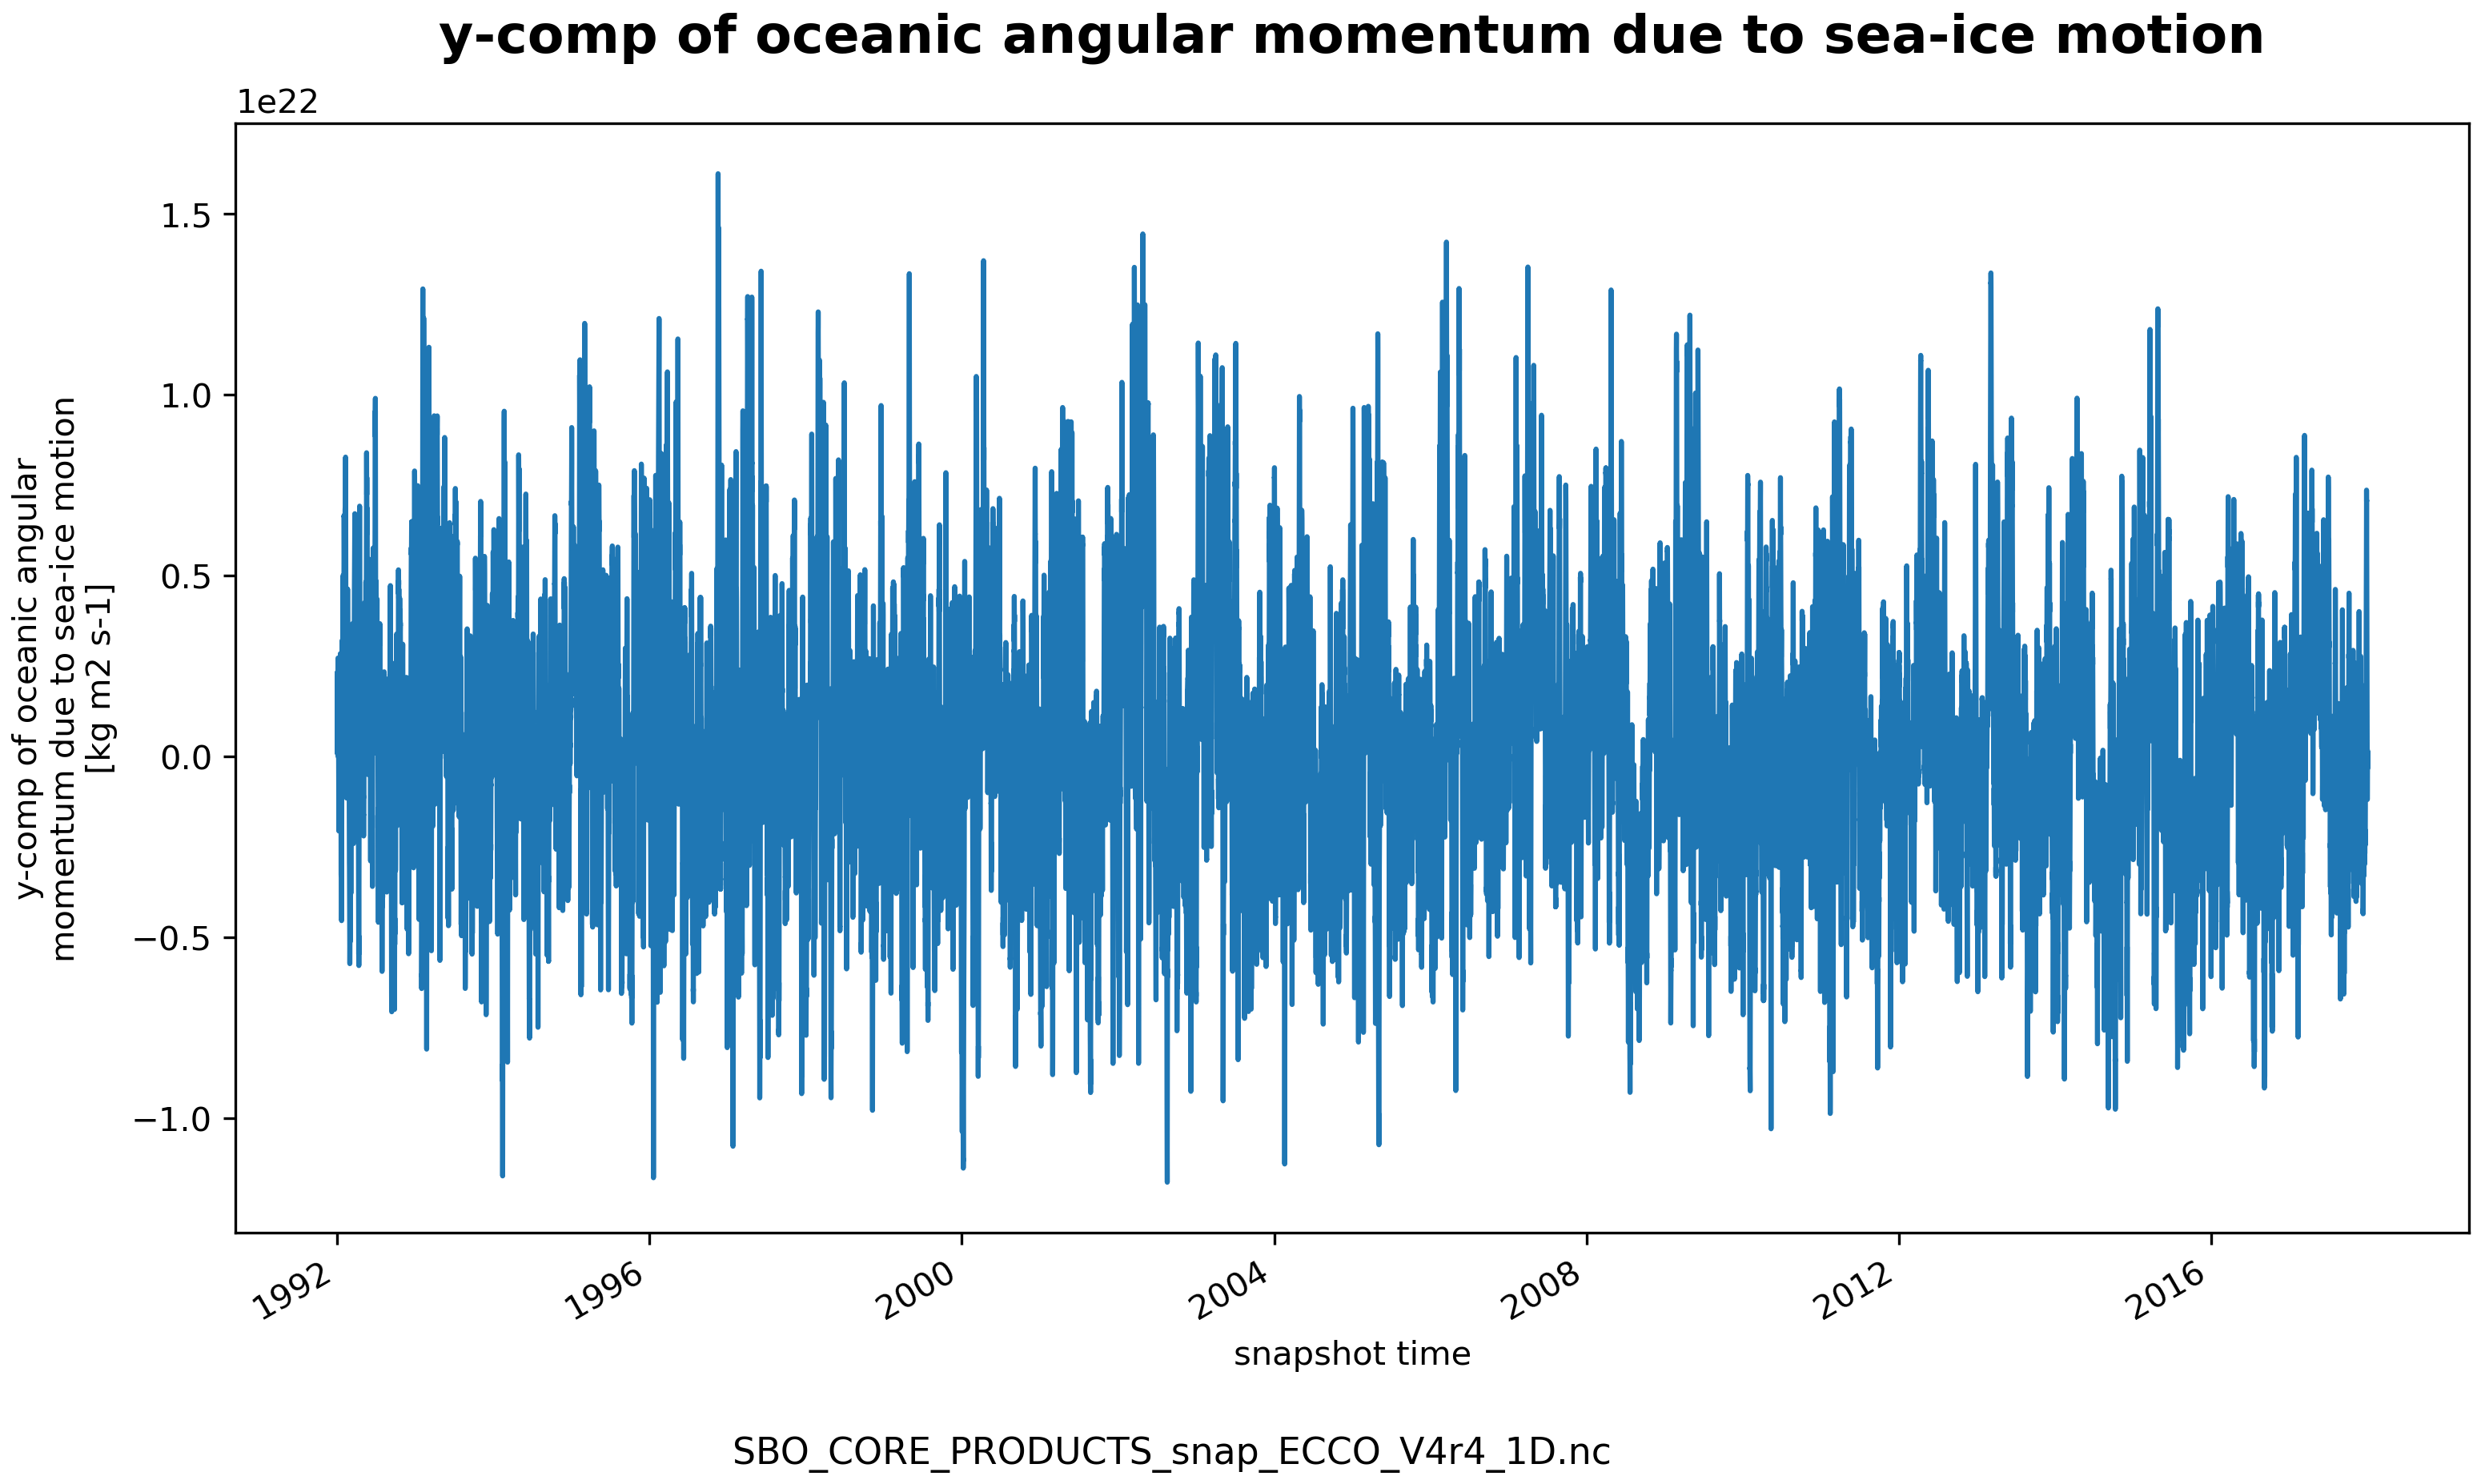
\includegraphics[scale=0.55]{../images/plots/oneD_plots/SBO_Core_Products/yoamc_si.png}
\caption{Dataset: SBO\_CORE\_PRODUCTS Variable: yoamc\_si}
\label{tab:table-SBO_CORE_PRODUCTS_yoamc_si-Plot}
\end{figure}
\pagebreak
\subsubsection{1D Variable yoamp}
\begin{longtable}{|m{0.06\textwidth}|m{0.41\textwidth}|m{0.39\textwidth}|m{0.06\textwidth}|}
\caption{CDL description of SBO\_CORE\_PRODUCTS's yoamp variable}
\label{tab:table-SBO_CORE_PRODUCTS_yoamp} \\ 
\hline \endhead \hline \endfoot
\rowcolor{lightgray} \textbf{Storage Type} & \textbf{Variable Name} & \textbf{Description} & \textbf{Unit} \\ \hline
float64 & yoamp & y-comp of oceanic angular momentum due to pressure & kg m2 s-1 \\ \hline
\rowcolor{lightgray}  \multicolumn{4}{|p{1.00\textwidth}|}{\textbf{CDL Description}} \\ \hline
\multicolumn{4}{|p{1.00\textwidth}|}{\makecell{\parbox{1\textwidth}{float64 yoamp(time)\\
\hspace*{0.5cm}yoamp: \_FillValue = 9.969209968386869e+36\\
\hspace*{0.5cm}yoamp: coverage\_content\_type = modelResult\\
\hspace*{0.5cm}yoamp: long\_name = y: comp of oceanic angular momentum due to pressure\\
\hspace*{0.5cm}yoamp: units = kg m2 s: 1\\
\hspace*{0.5cm}yoamp: valid\_min = 1.0476388397938864e+29\\
\hspace*{0.5cm}yoamp: valid\_max = 1.0478581623131764e+29\\
\hspace*{0.5cm}yoamp: coordinates = time}}} \\ \hline
\rowcolor{lightgray} \multicolumn{4}{|p{1.00\textwidth}|}{\textbf{Comments}} \\ \hline
\multicolumn{4}{|p{1\textwidth}|}{N/A} \\ \hline
\end{longtable}

\begin{figure}[H]
\centering
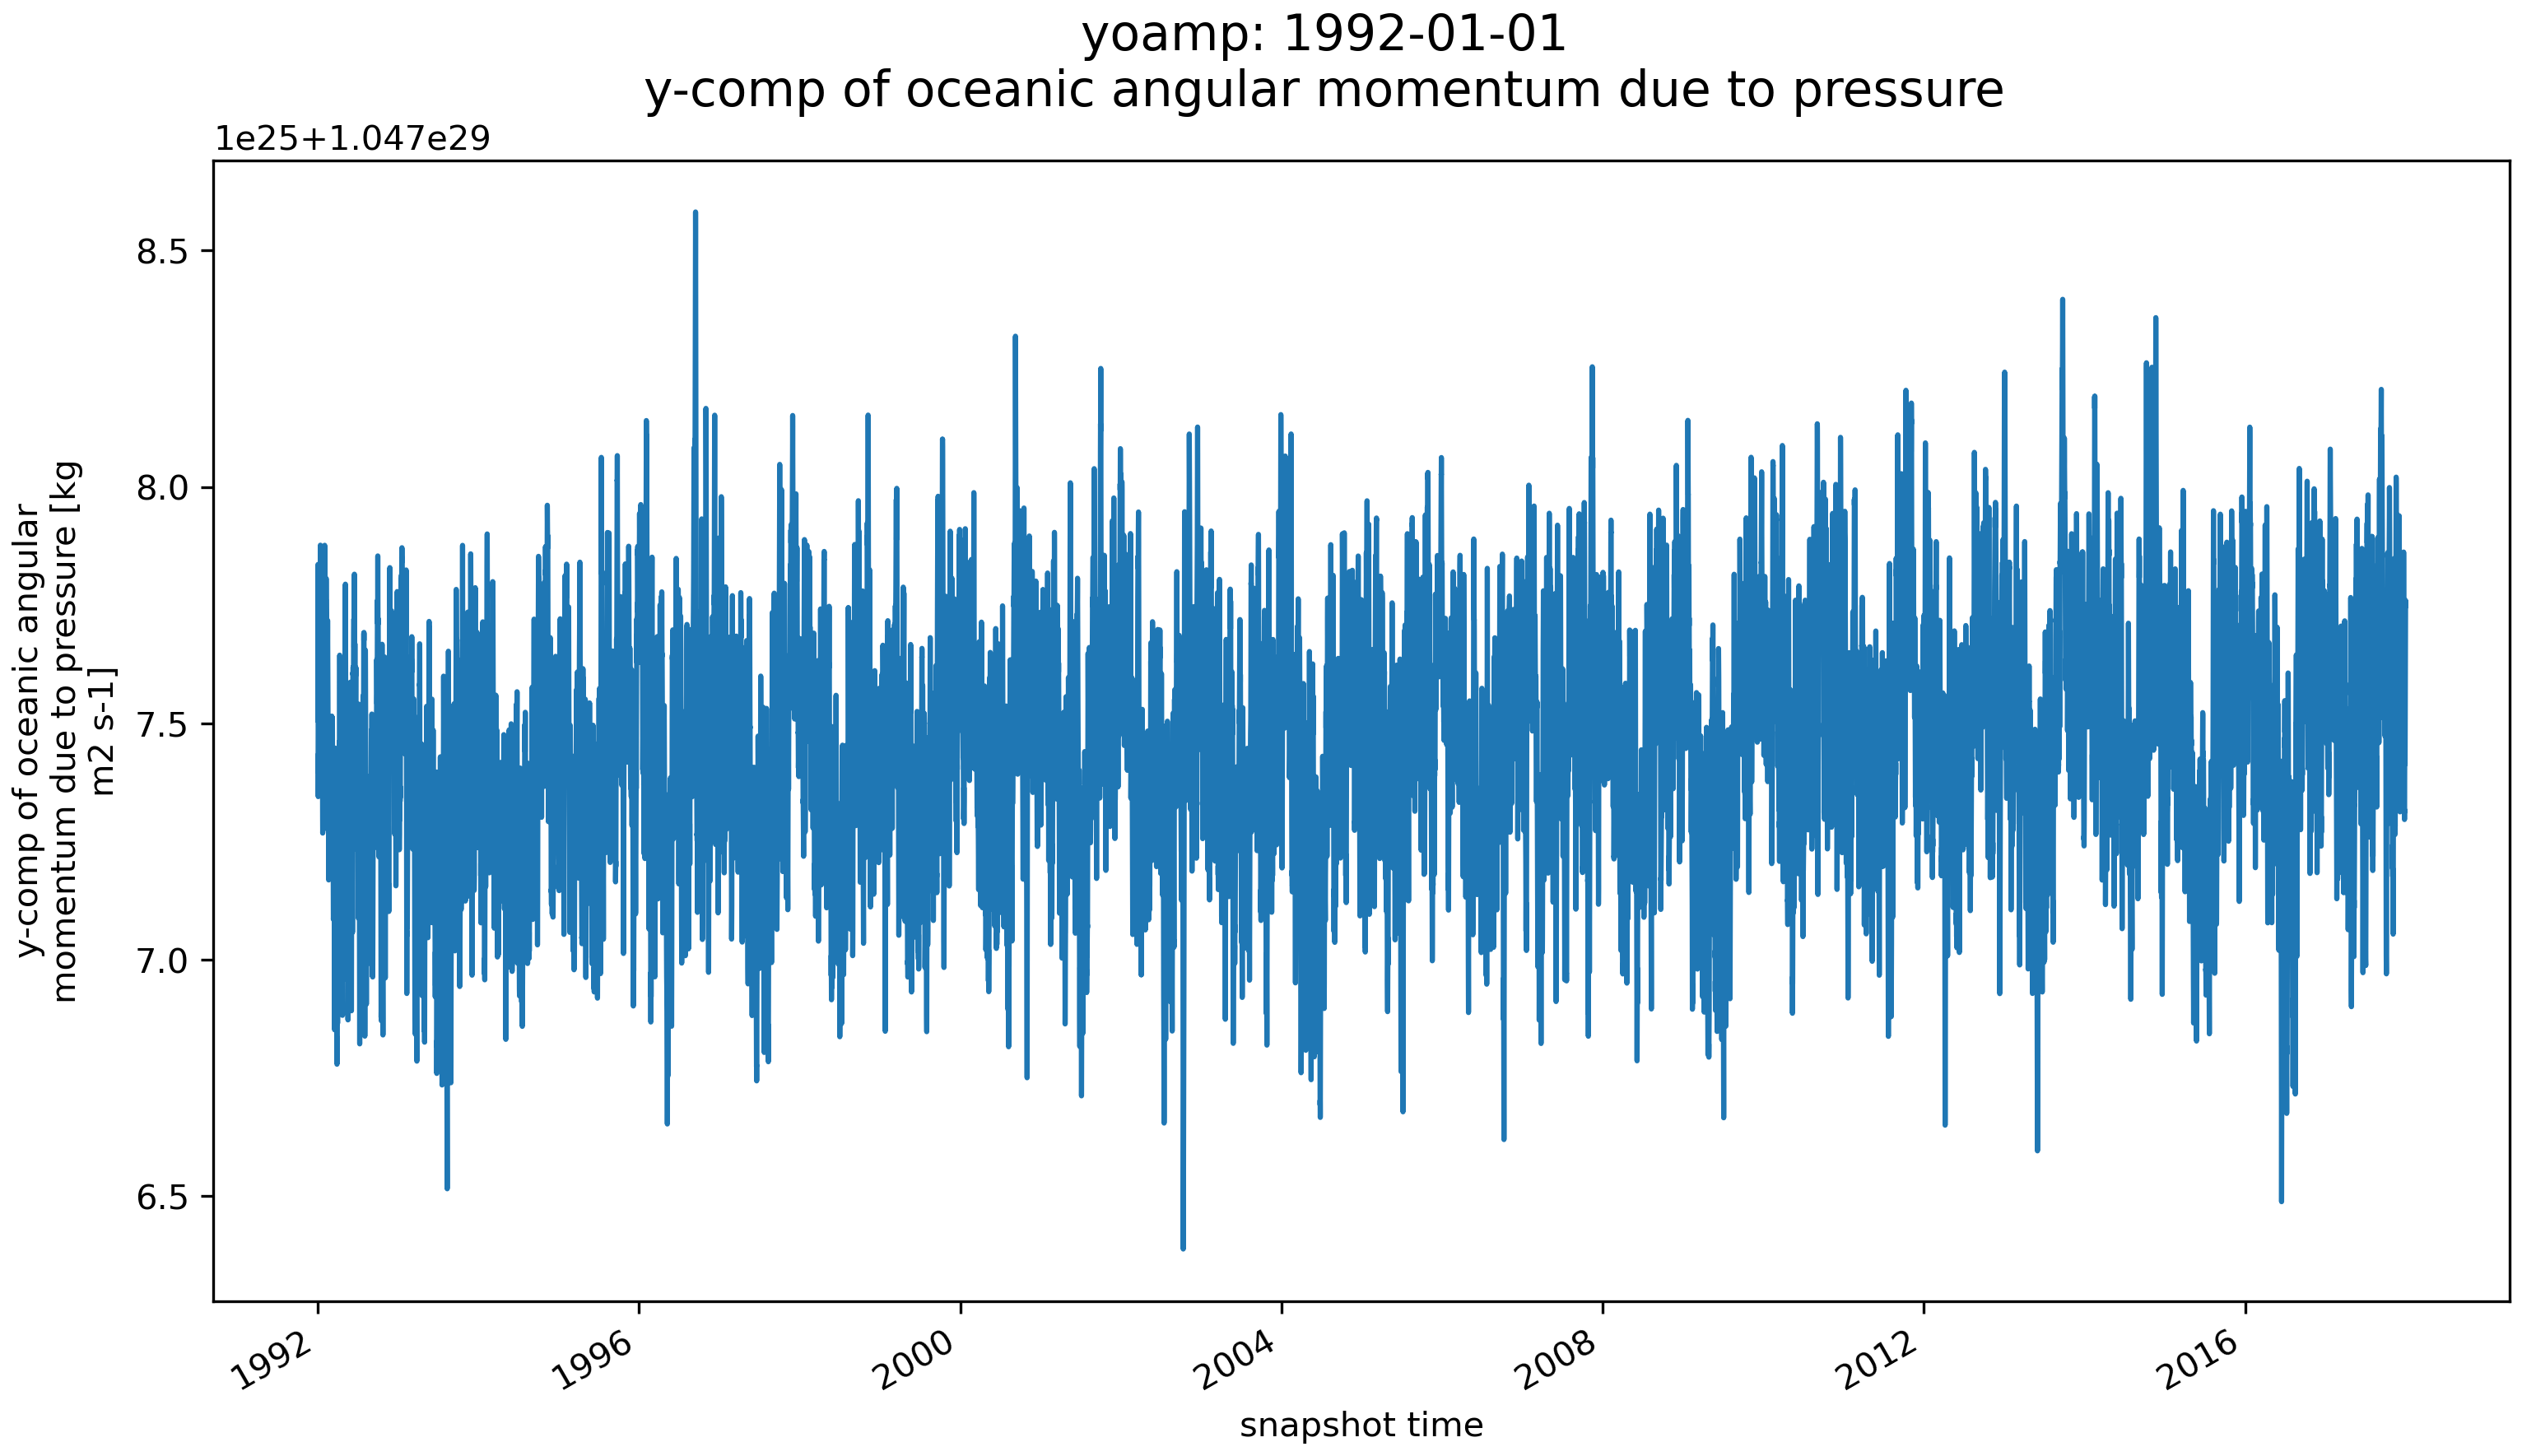
\includegraphics[scale=0.55]{../images/plots/oneD_plots/SBO_Core_Products/yoamp.png}
\caption{Dataset: SBO\_CORE\_PRODUCTS Variable: yoamp}
\label{tab:table-SBO_CORE_PRODUCTS_yoamp-Plot}
\end{figure}
\pagebreak
\subsubsection{1D Variable yoamp\_dsl}
\begin{longtable}{|m{0.06\textwidth}|m{0.41\textwidth}|m{0.39\textwidth}|m{0.06\textwidth}|}
\caption{CDL description of SBO\_CORE\_PRODUCTS's yoamp\_dsl variable}
\label{tab:table-SBO_CORE_PRODUCTS_yoamp_dsl} \\ 
\hline \endhead \hline \endfoot
\rowcolor{lightgray} \textbf{Storage Type} & \textbf{Variable Name} & \textbf{Description} & \textbf{Unit} \\ \hline
float64 & yoamp\_dsl & y-comp of oceanic angular momentum due to pressure based on dynamic (IB-corrected) sea level & kg m2 s-1 \\ \hline
\rowcolor{lightgray}  \multicolumn{4}{|p{1.00\textwidth}|}{\textbf{CDL Description}} \\ \hline
\multicolumn{4}{|p{1.00\textwidth}|}{\makecell{\parbox{1\textwidth}{float64 yoamp\_dsl(time)\\
\hspace*{0.5cm}yoamp\_dsl: \_FillValue = 9.969209968386869e+36\\
\hspace*{0.5cm}yoamp\_dsl: coverage\_content\_type = modelResult\\
\hspace*{0.5cm}yoamp\_dsl: long\_name = y: comp of oceanic angular momentum due to pressure based on dynamic (IB: corrected) sea level\\
\hspace*{0.5cm}yoamp\_dsl: units = kg m2 s: 1\\
\hspace*{0.5cm}yoamp\_dsl: valid\_min = 1.0476994334049981e+29\\
\hspace*{0.5cm}yoamp\_dsl: valid\_max = 1.0478187262074598e+29\\
\hspace*{0.5cm}yoamp\_dsl: coordinates = time}}} \\ \hline
\rowcolor{lightgray} \multicolumn{4}{|p{1.00\textwidth}|}{\textbf{Comments}} \\ \hline
\multicolumn{4}{|p{1\textwidth}|}{N/A} \\ \hline
\end{longtable}

\begin{figure}[H]
\centering
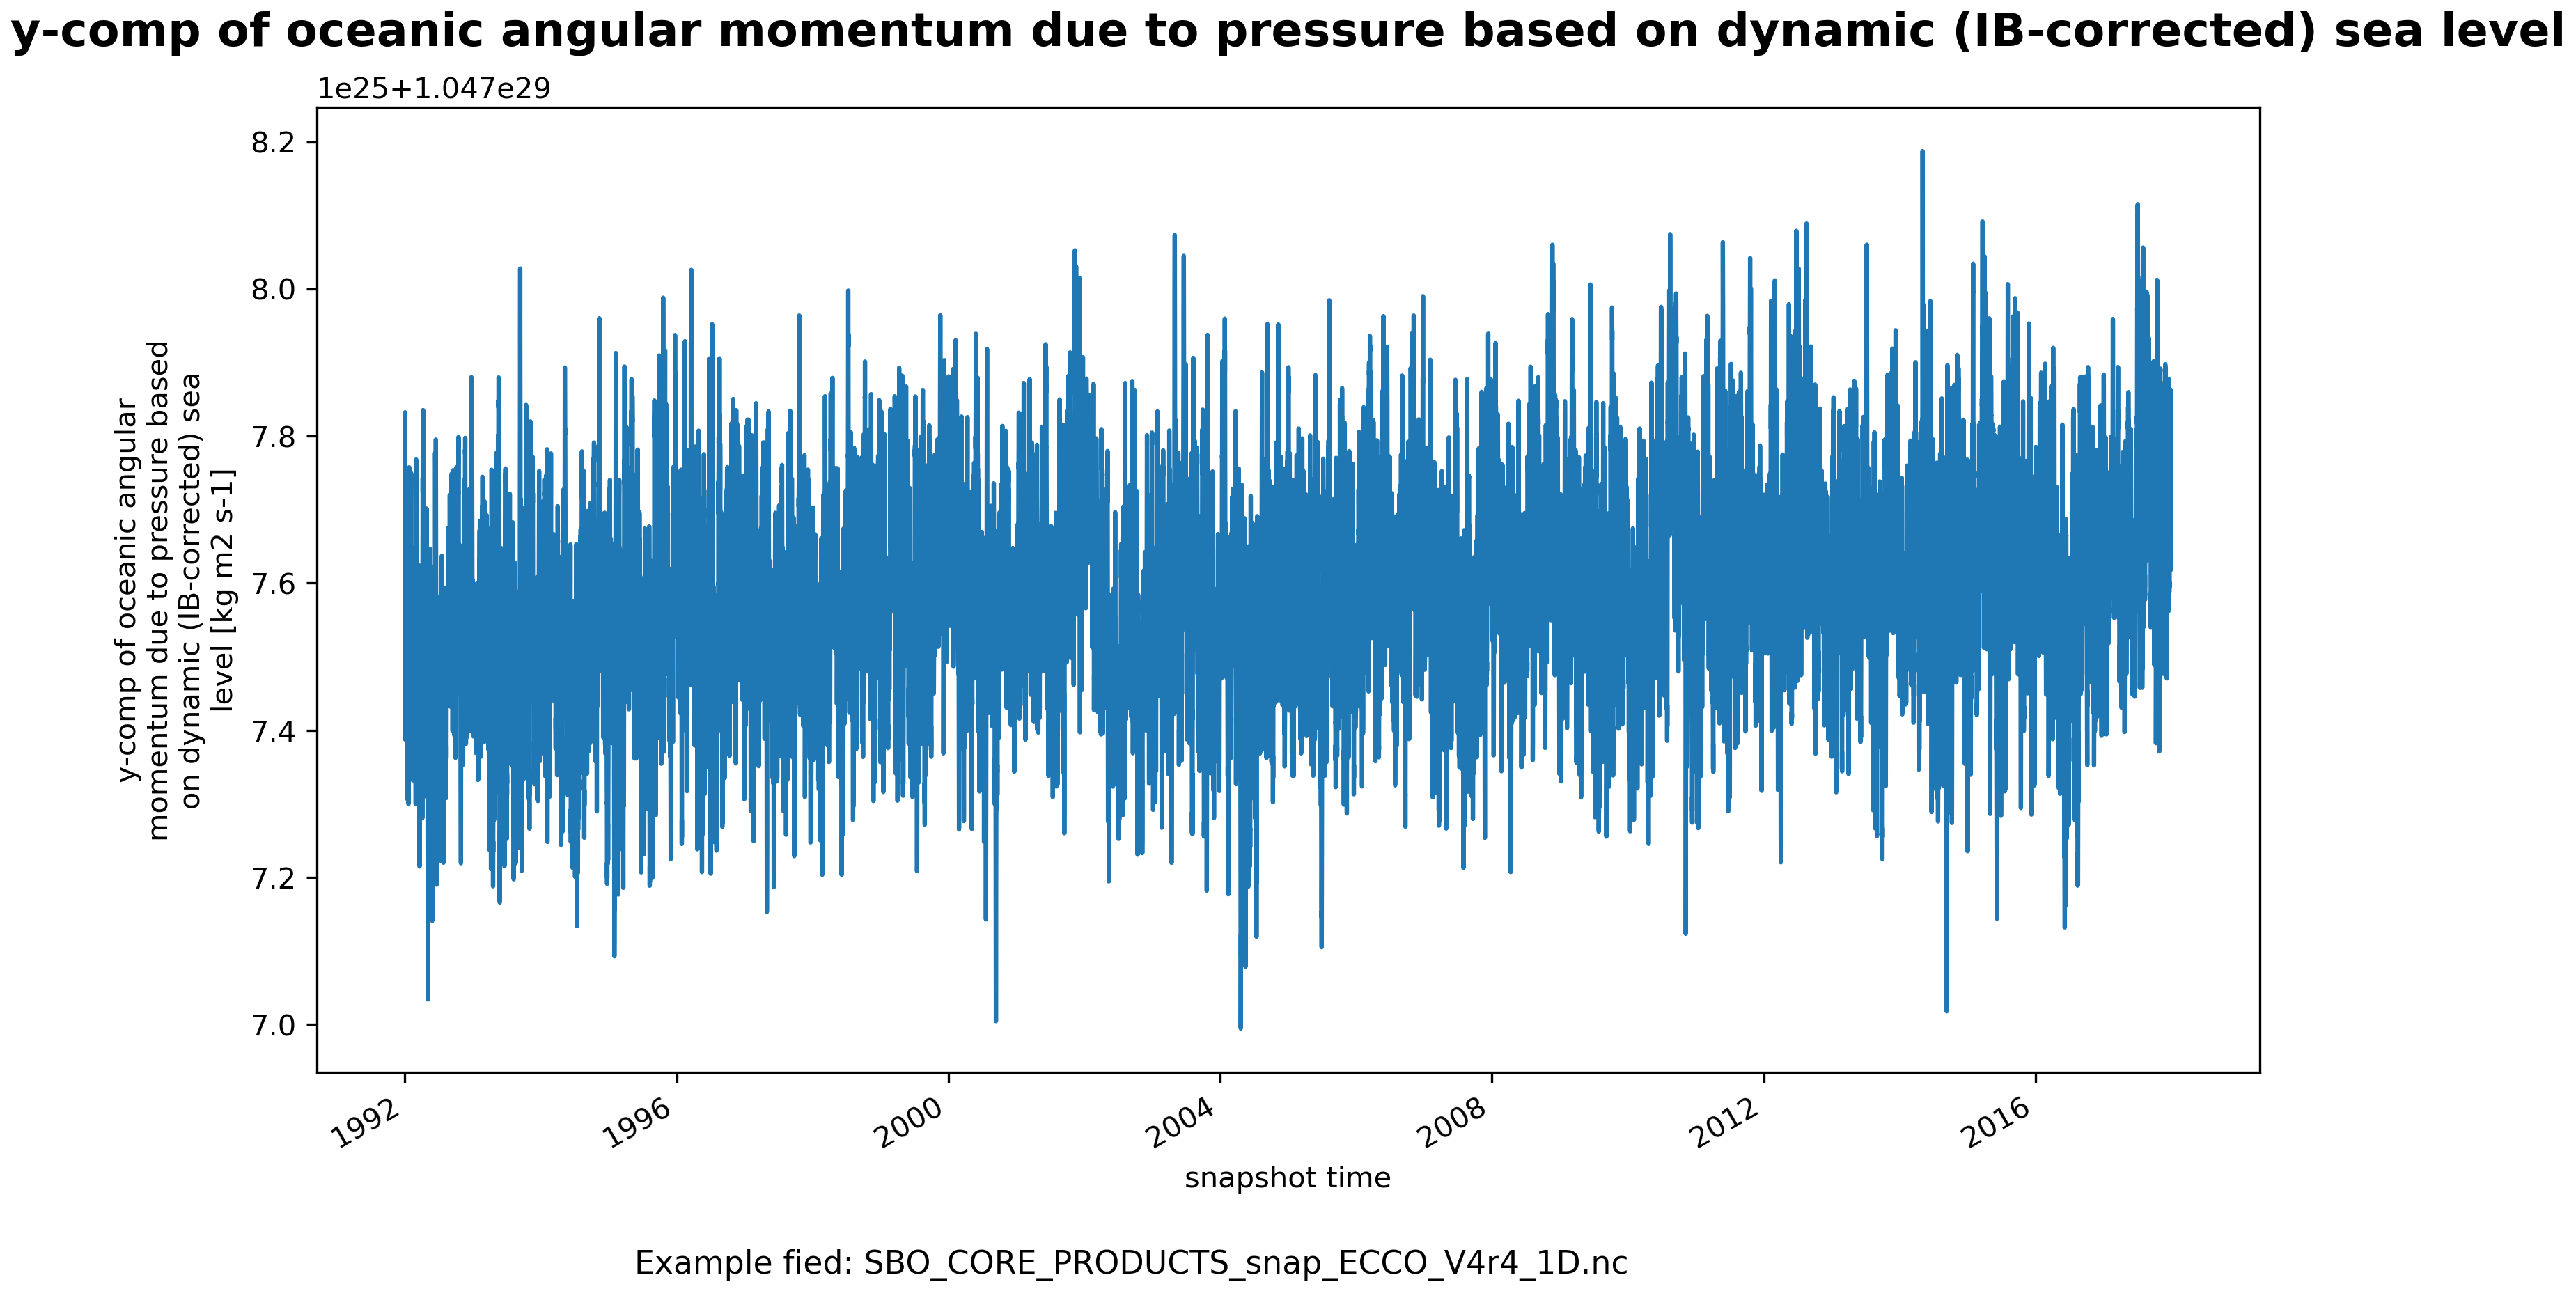
\includegraphics[scale=0.55]{../images/plots/oneD_plots/SBO_Core_Products/yoamp_dsl.png}
\caption{Dataset: SBO\_CORE\_PRODUCTS Variable: yoamp\_dsl}
\label{tab:table-SBO_CORE_PRODUCTS_yoamp_dsl-Plot}
\end{figure}
\pagebreak
\subsubsection{1D Variable yoamp\_fw}
\begin{longtable}{|m{0.06\textwidth}|m{0.41\textwidth}|m{0.39\textwidth}|m{0.06\textwidth}|}
\caption{CDL description of SBO\_CORE\_PRODUCTS's yoamp\_fw variable}
\label{tab:table-SBO_CORE_PRODUCTS_yoamp_fw} \\ 
\hline \endhead \hline \endfoot
\rowcolor{lightgray} \textbf{Storage Type} & \textbf{Variable Name} & \textbf{Description} & \textbf{Unit} \\ \hline
float64 & yoamp\_fw & y-comp of oceanic angular momentum due to freshwater flux & kg m2 s-1 \\ \hline
\rowcolor{lightgray}  \multicolumn{4}{|p{1.00\textwidth}|}{\textbf{CDL Description}} \\ \hline
\multicolumn{4}{|p{1.00\textwidth}|}{\makecell{\parbox{1\textwidth}{float64 yoamp\_fw(time)\\
\hspace*{0.5cm}yoamp\_fw: \_FillValue = 9.969209968386869e+36\\
\hspace*{0.5cm}yoamp\_fw: coverage\_content\_type = modelResult\\
\hspace*{0.5cm}yoamp\_fw: long\_name = y: comp of oceanic angular momentum due to freshwater flux\\
\hspace*{0.5cm}yoamp\_fw: units = kg m2 s: 1\\
\hspace*{0.5cm}yoamp\_fw: valid\_min = 2.6255410225894626e+24\\
\hspace*{0.5cm}yoamp\_fw: valid\_max = 4.872705717529432e+24\\
\hspace*{0.5cm}yoamp\_fw: coordinates = time}}} \\ \hline
\rowcolor{lightgray} \multicolumn{4}{|p{1.00\textwidth}|}{\textbf{Comments}} \\ \hline
\multicolumn{4}{|p{1\textwidth}|}{N/A} \\ \hline
\end{longtable}

\begin{figure}[H]
\centering
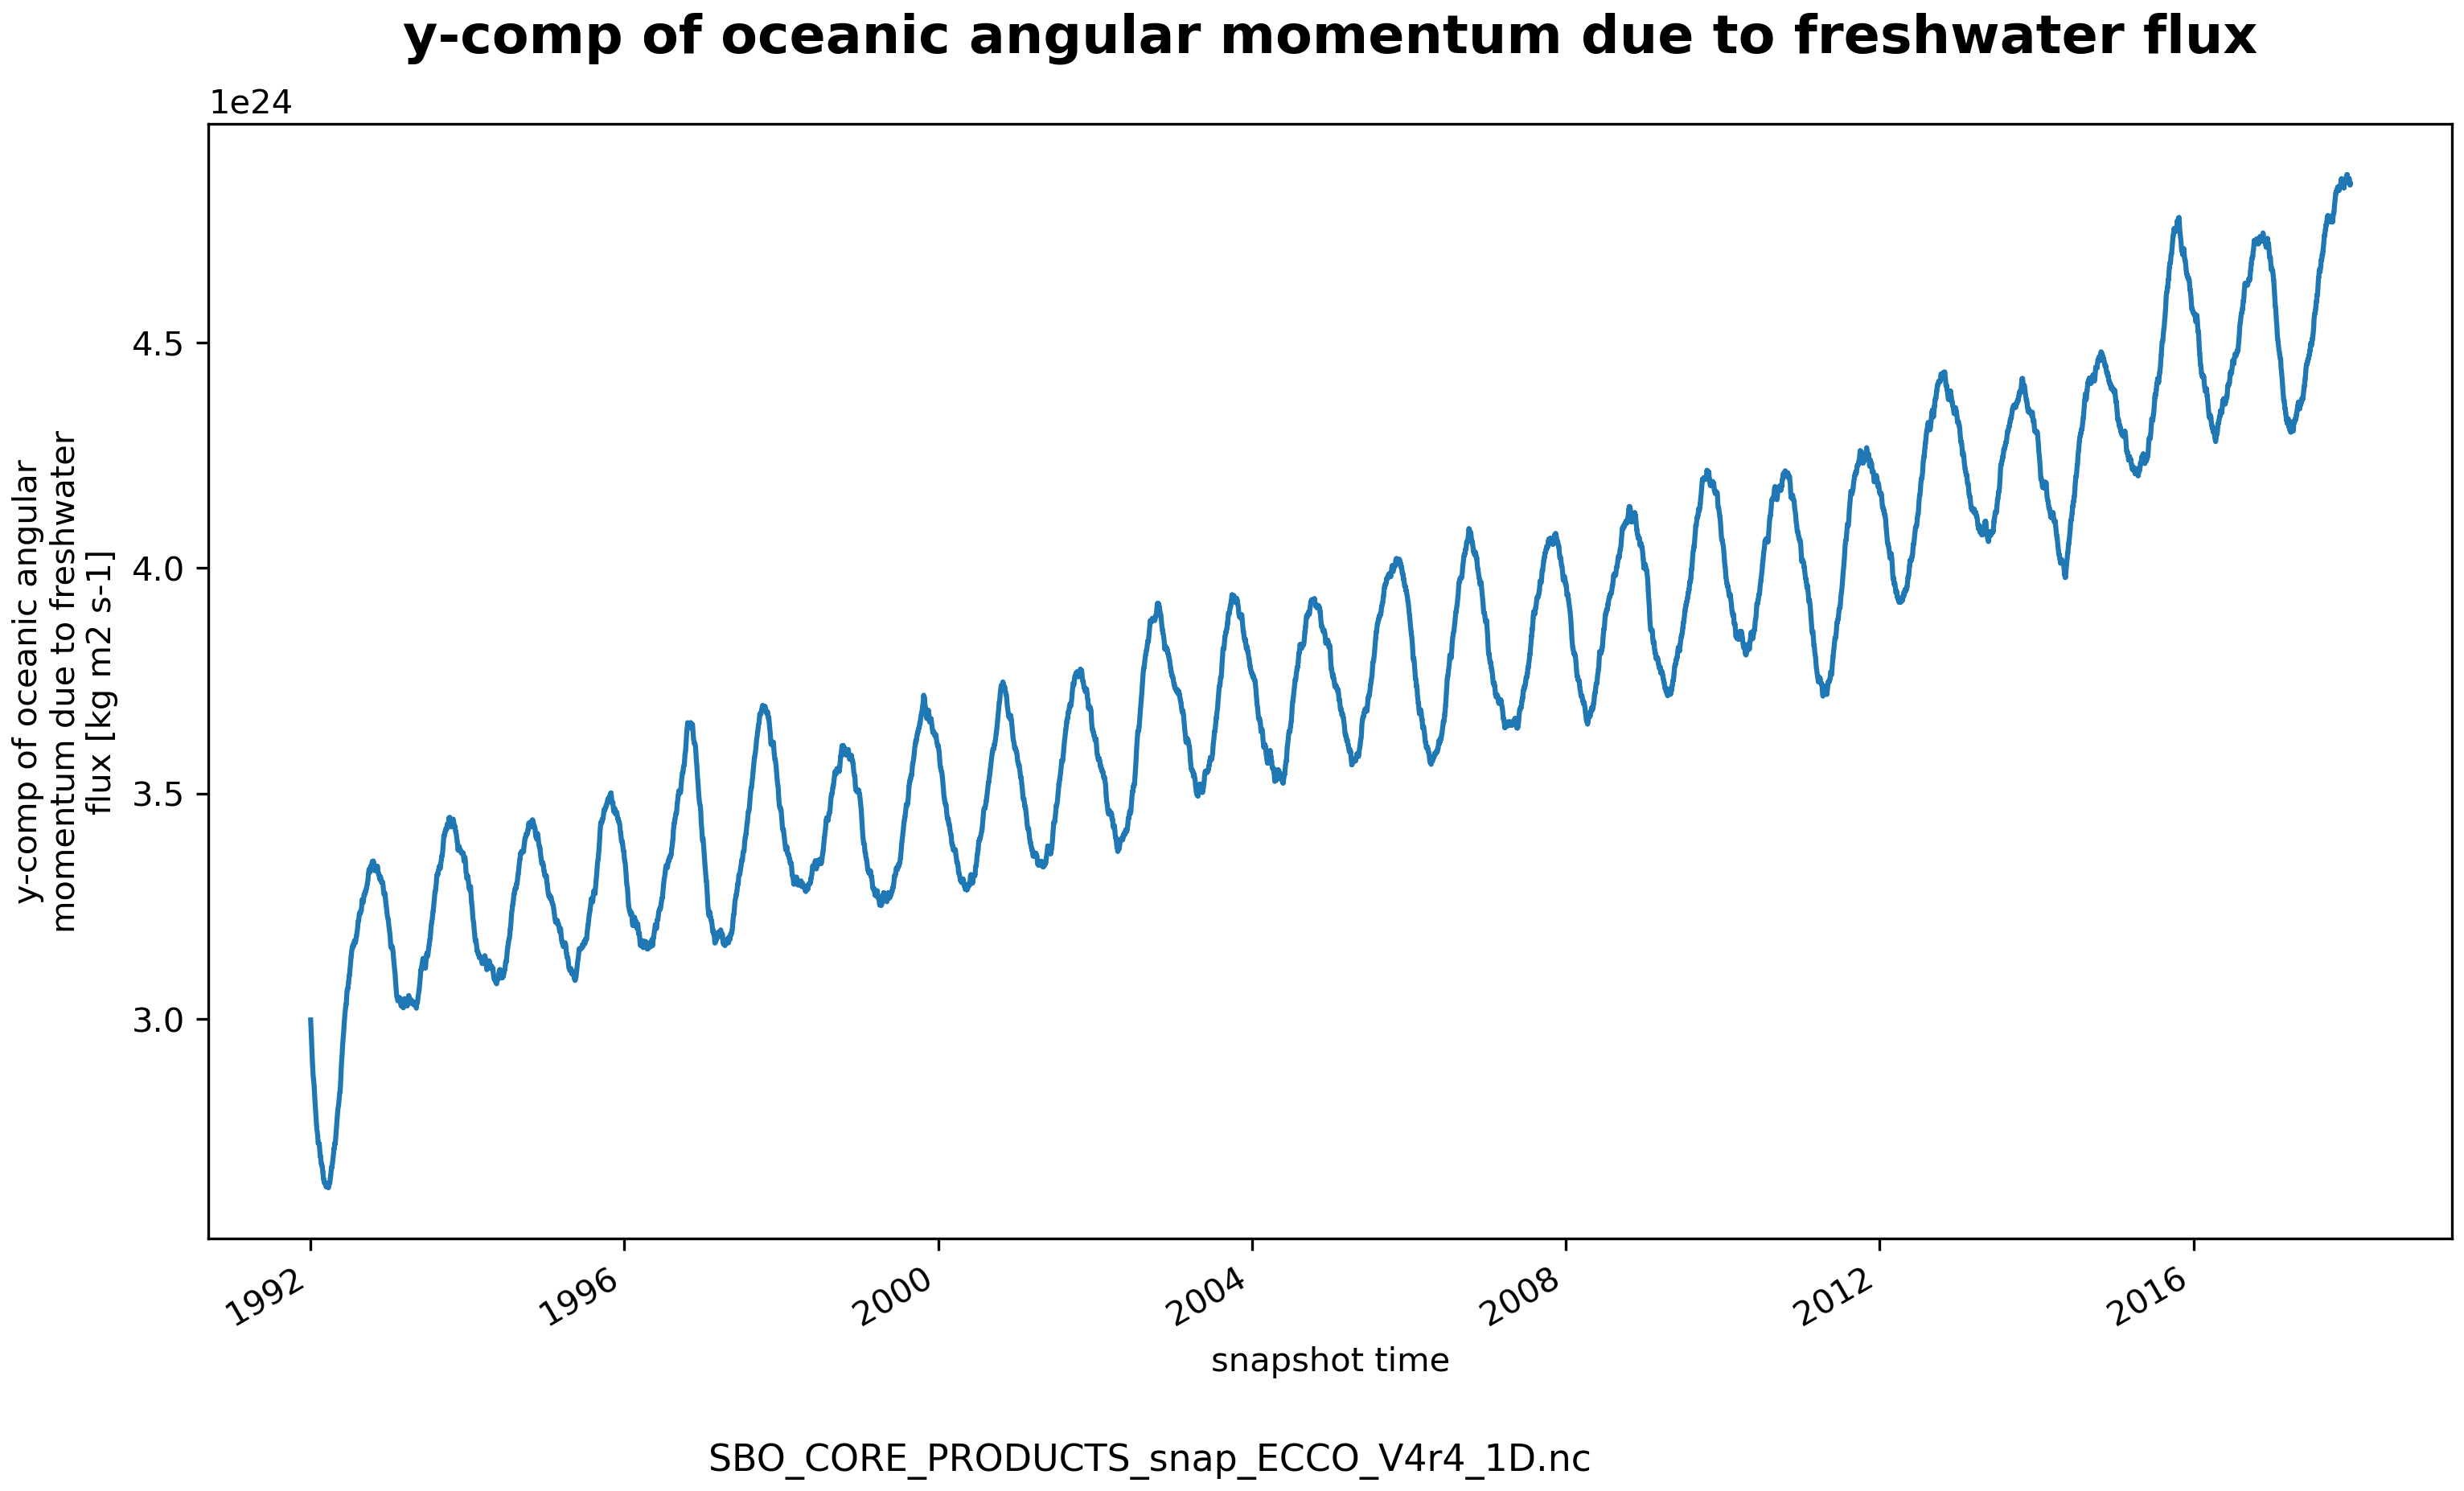
\includegraphics[scale=0.55]{../images/plots/oneD_plots/SBO_Core_Products/yoamp_fw.png}
\caption{Dataset: SBO\_CORE\_PRODUCTS Variable: yoamp\_fw}
\label{tab:table-SBO_CORE_PRODUCTS_yoamp_fw-Plot}
\end{figure}
\pagebreak
\subsubsection{1D Variable zcom}
\begin{longtable}{|m{0.06\textwidth}|m{0.41\textwidth}|m{0.39\textwidth}|m{0.06\textwidth}|}
\caption{CDL description of SBO\_CORE\_PRODUCTS's zcom variable}
\label{tab:table-SBO_CORE_PRODUCTS_zcom} \\ 
\hline \endhead \hline \endfoot
\rowcolor{lightgray} \textbf{Storage Type} & \textbf{Variable Name} & \textbf{Description} & \textbf{Unit} \\ \hline
float64 & zcom & z-comp of center-of-mass of ocean & m \\ \hline
\rowcolor{lightgray}  \multicolumn{4}{|p{1.00\textwidth}|}{\textbf{CDL Description}} \\ \hline
\multicolumn{4}{|p{1.00\textwidth}|}{\makecell{\parbox{1\textwidth}{float64 zcom(time)\\
\hspace*{0.5cm}zcom: \_FillValue = 9.969209968386869e+36\\
\hspace*{0.5cm}zcom: coverage\_content\_type = modelResult\\
\hspace*{0.5cm}zcom: long\_name = z: comp of center: of: mass of ocean\\
\hspace*{0.5cm}zcom: units = m\\
\hspace*{0.5cm}zcom: valid\_min = : 875420.3898804963\\
\hspace*{0.5cm}zcom: valid\_max = : 875350.3238026679\\
\hspace*{0.5cm}zcom: coordinates = time}}} \\ \hline
\rowcolor{lightgray} \multicolumn{4}{|p{1.00\textwidth}|}{\textbf{Comments}} \\ \hline
\multicolumn{4}{|p{1\textwidth}|}{N/A} \\ \hline
\end{longtable}

\begin{figure}[H]
\centering
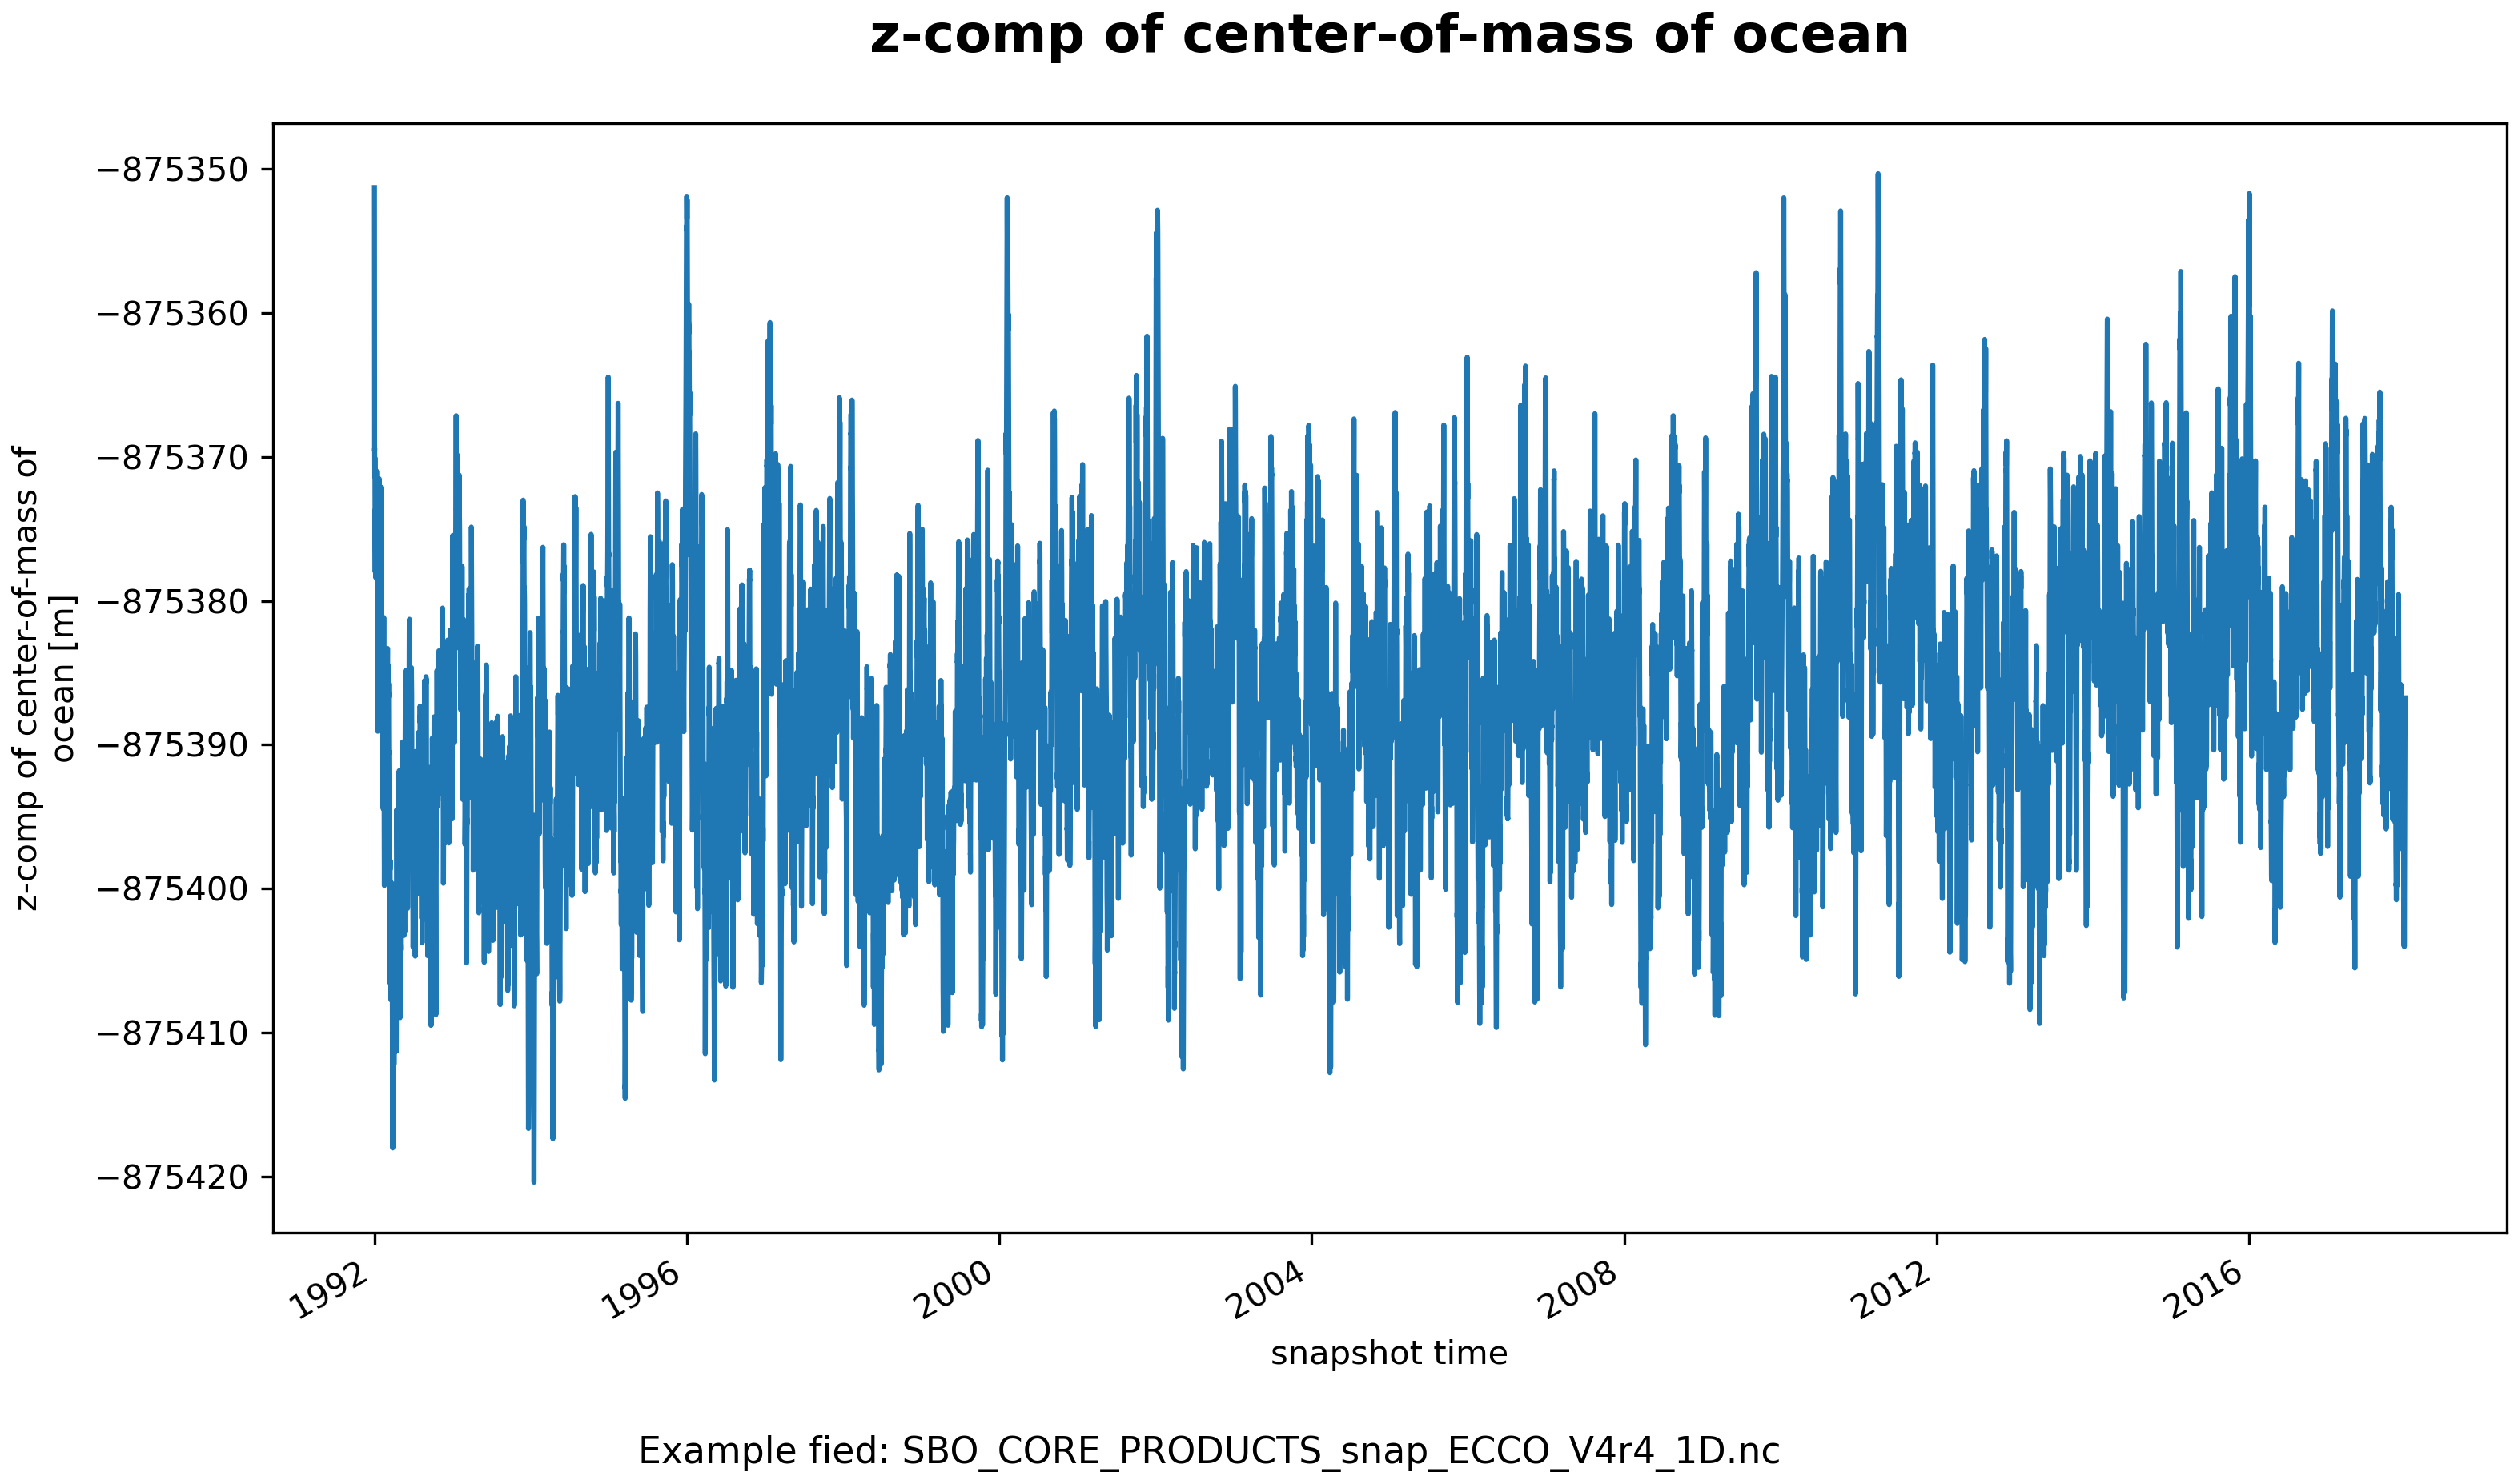
\includegraphics[scale=0.55]{../images/plots/oneD_plots/SBO_Core_Products/zcom.png}
\caption{Dataset: SBO\_CORE\_PRODUCTS Variable: zcom}
\label{tab:table-SBO_CORE_PRODUCTS_zcom-Plot}
\end{figure}
\pagebreak
\subsubsection{1D Variable zcom\_fw}
\begin{longtable}{|m{0.06\textwidth}|m{0.41\textwidth}|m{0.39\textwidth}|m{0.06\textwidth}|}
\caption{CDL description of SBO\_CORE\_PRODUCTS's zcom\_fw variable}
\label{tab:table-SBO_CORE_PRODUCTS_zcom_fw} \\ 
\hline \endhead \hline \endfoot
\rowcolor{lightgray} \textbf{Storage Type} & \textbf{Variable Name} & \textbf{Description} & \textbf{Unit} \\ \hline
float64 & zcom\_fw & z-comp of center-of-mass of freshater flux & m \\ \hline
\rowcolor{lightgray}  \multicolumn{4}{|p{1.00\textwidth}|}{\textbf{CDL Description}} \\ \hline
\multicolumn{4}{|p{1.00\textwidth}|}{\makecell{\parbox{1\textwidth}{float64 zcom\_fw(time)\\
\hspace*{0.5cm}zcom\_fw: \_FillValue = 9.969209968386869e+36\\
\hspace*{0.5cm}zcom\_fw: coverage\_content\_type = modelResult\\
\hspace*{0.5cm}zcom\_fw: long\_name = z: comp of center: of: mass of freshater flux\\
\hspace*{0.5cm}zcom\_fw: units = m\\
\hspace*{0.5cm}zcom\_fw: valid\_min = : 648386.5781734617\\
\hspace*{0.5cm}zcom\_fw: valid\_max = : 648386.5781734567\\
\hspace*{0.5cm}zcom\_fw: coordinates = time}}} \\ \hline
\rowcolor{lightgray} \multicolumn{4}{|p{1.00\textwidth}|}{\textbf{Comments}} \\ \hline
\multicolumn{4}{|p{1\textwidth}|}{N/A} \\ \hline
\end{longtable}

\begin{figure}[H]
\centering
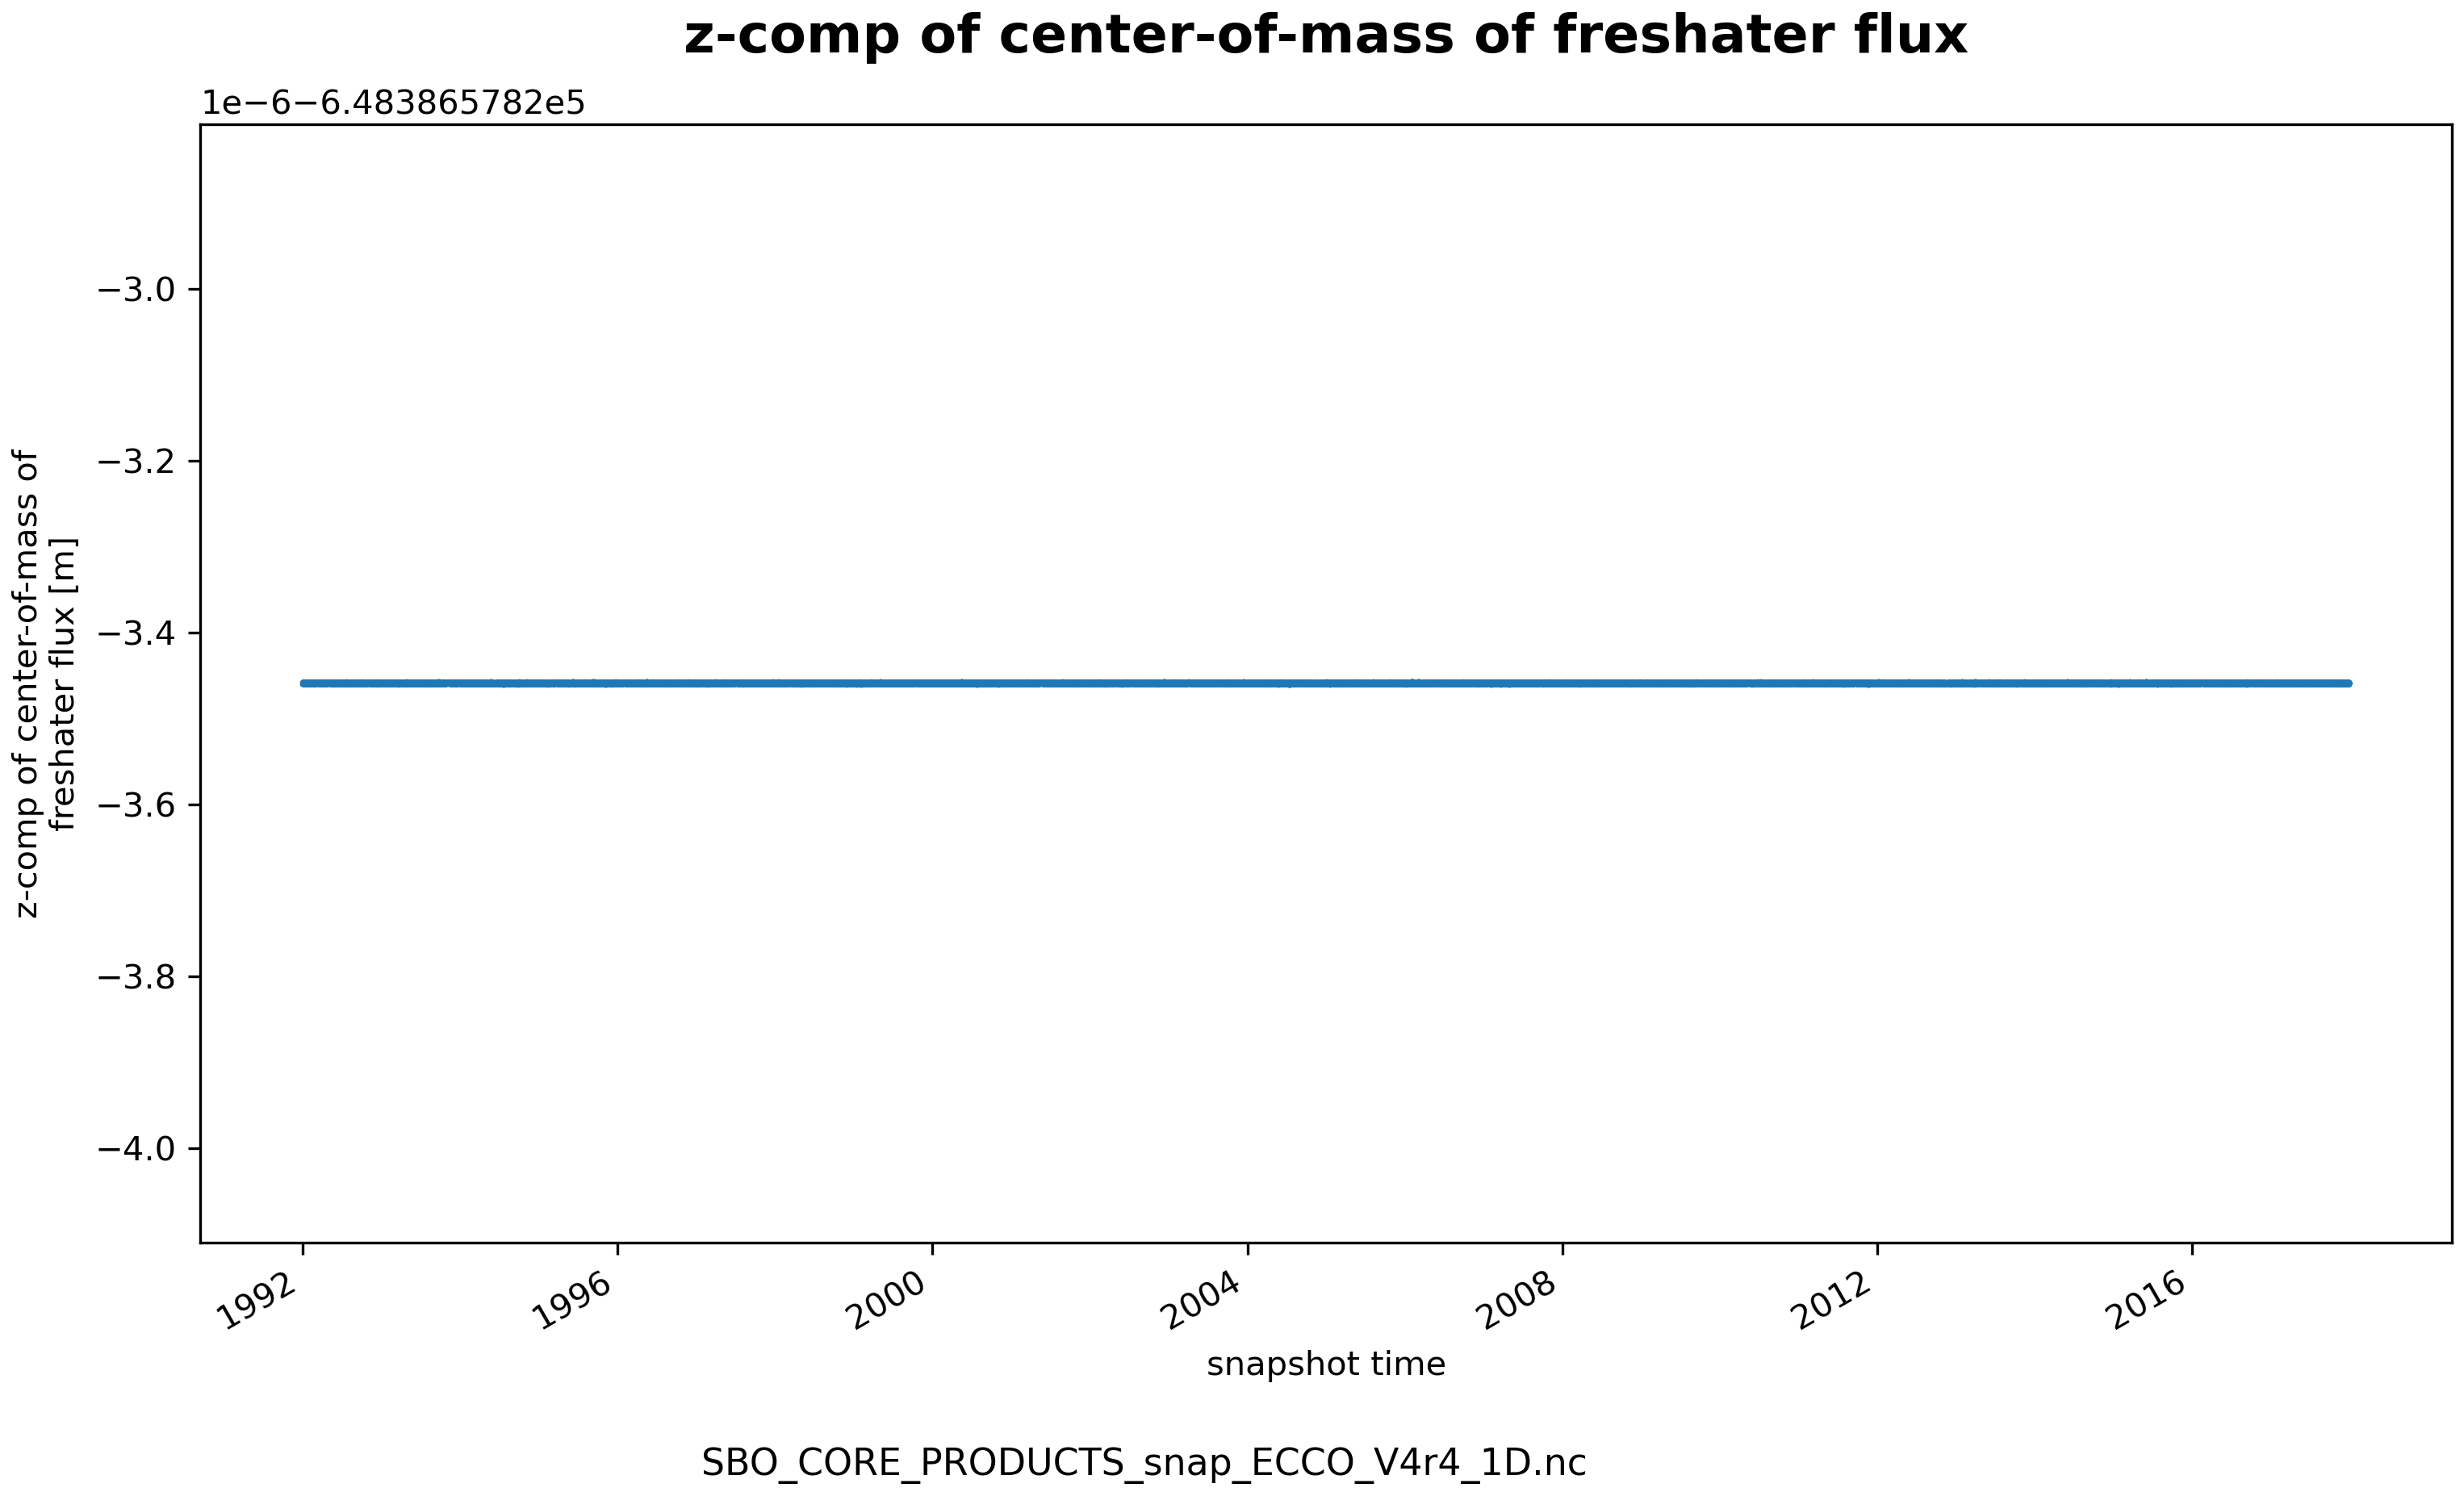
\includegraphics[scale=0.55]{../images/plots/oneD_plots/SBO_Core_Products/zcom_fw.png}
\caption{Dataset: SBO\_CORE\_PRODUCTS Variable: zcom\_fw}
\label{tab:table-SBO_CORE_PRODUCTS_zcom_fw-Plot}
\end{figure}
\pagebreak
\subsubsection{1D Variable zoamc}
\begin{longtable}{|m{0.06\textwidth}|m{0.41\textwidth}|m{0.39\textwidth}|m{0.06\textwidth}|}
\caption{CDL description of SBO\_CORE\_PRODUCTS's zoamc variable}
\label{tab:table-SBO_CORE_PRODUCTS_zoamc} \\ 
\hline \endhead \hline \endfoot
\rowcolor{lightgray} \textbf{Storage Type} & \textbf{Variable Name} & \textbf{Description} & \textbf{Unit} \\ \hline
float64 & zoamc & z-comp of oceanic angular momentum due to currents & kg m2 s-1 \\ \hline
\rowcolor{lightgray}  \multicolumn{4}{|p{1.00\textwidth}|}{\textbf{CDL Description}} \\ \hline
\multicolumn{4}{|p{1.00\textwidth}|}{\makecell{\parbox{1\textwidth}{float64 zoamc(time)\\
\hspace*{0.5cm}zoamc: \_FillValue = 9.969209968386869e+36\\
\hspace*{0.5cm}zoamc: coverage\_content\_type = modelResult\\
\hspace*{0.5cm}zoamc: long\_name = z: comp of oceanic angular momentum due to currents\\
\hspace*{0.5cm}zoamc: units = kg m2 s: 1\\
\hspace*{0.5cm}zoamc: valid\_min = 7.331764457927521e+24\\
\hspace*{0.5cm}zoamc: valid\_max = 2.207264300276968e+25\\
\hspace*{0.5cm}zoamc: coordinates = time}}} \\ \hline
\rowcolor{lightgray} \multicolumn{4}{|p{1.00\textwidth}|}{\textbf{Comments}} \\ \hline
\multicolumn{4}{|p{1\textwidth}|}{N/A} \\ \hline
\end{longtable}

\begin{figure}[H]
\centering
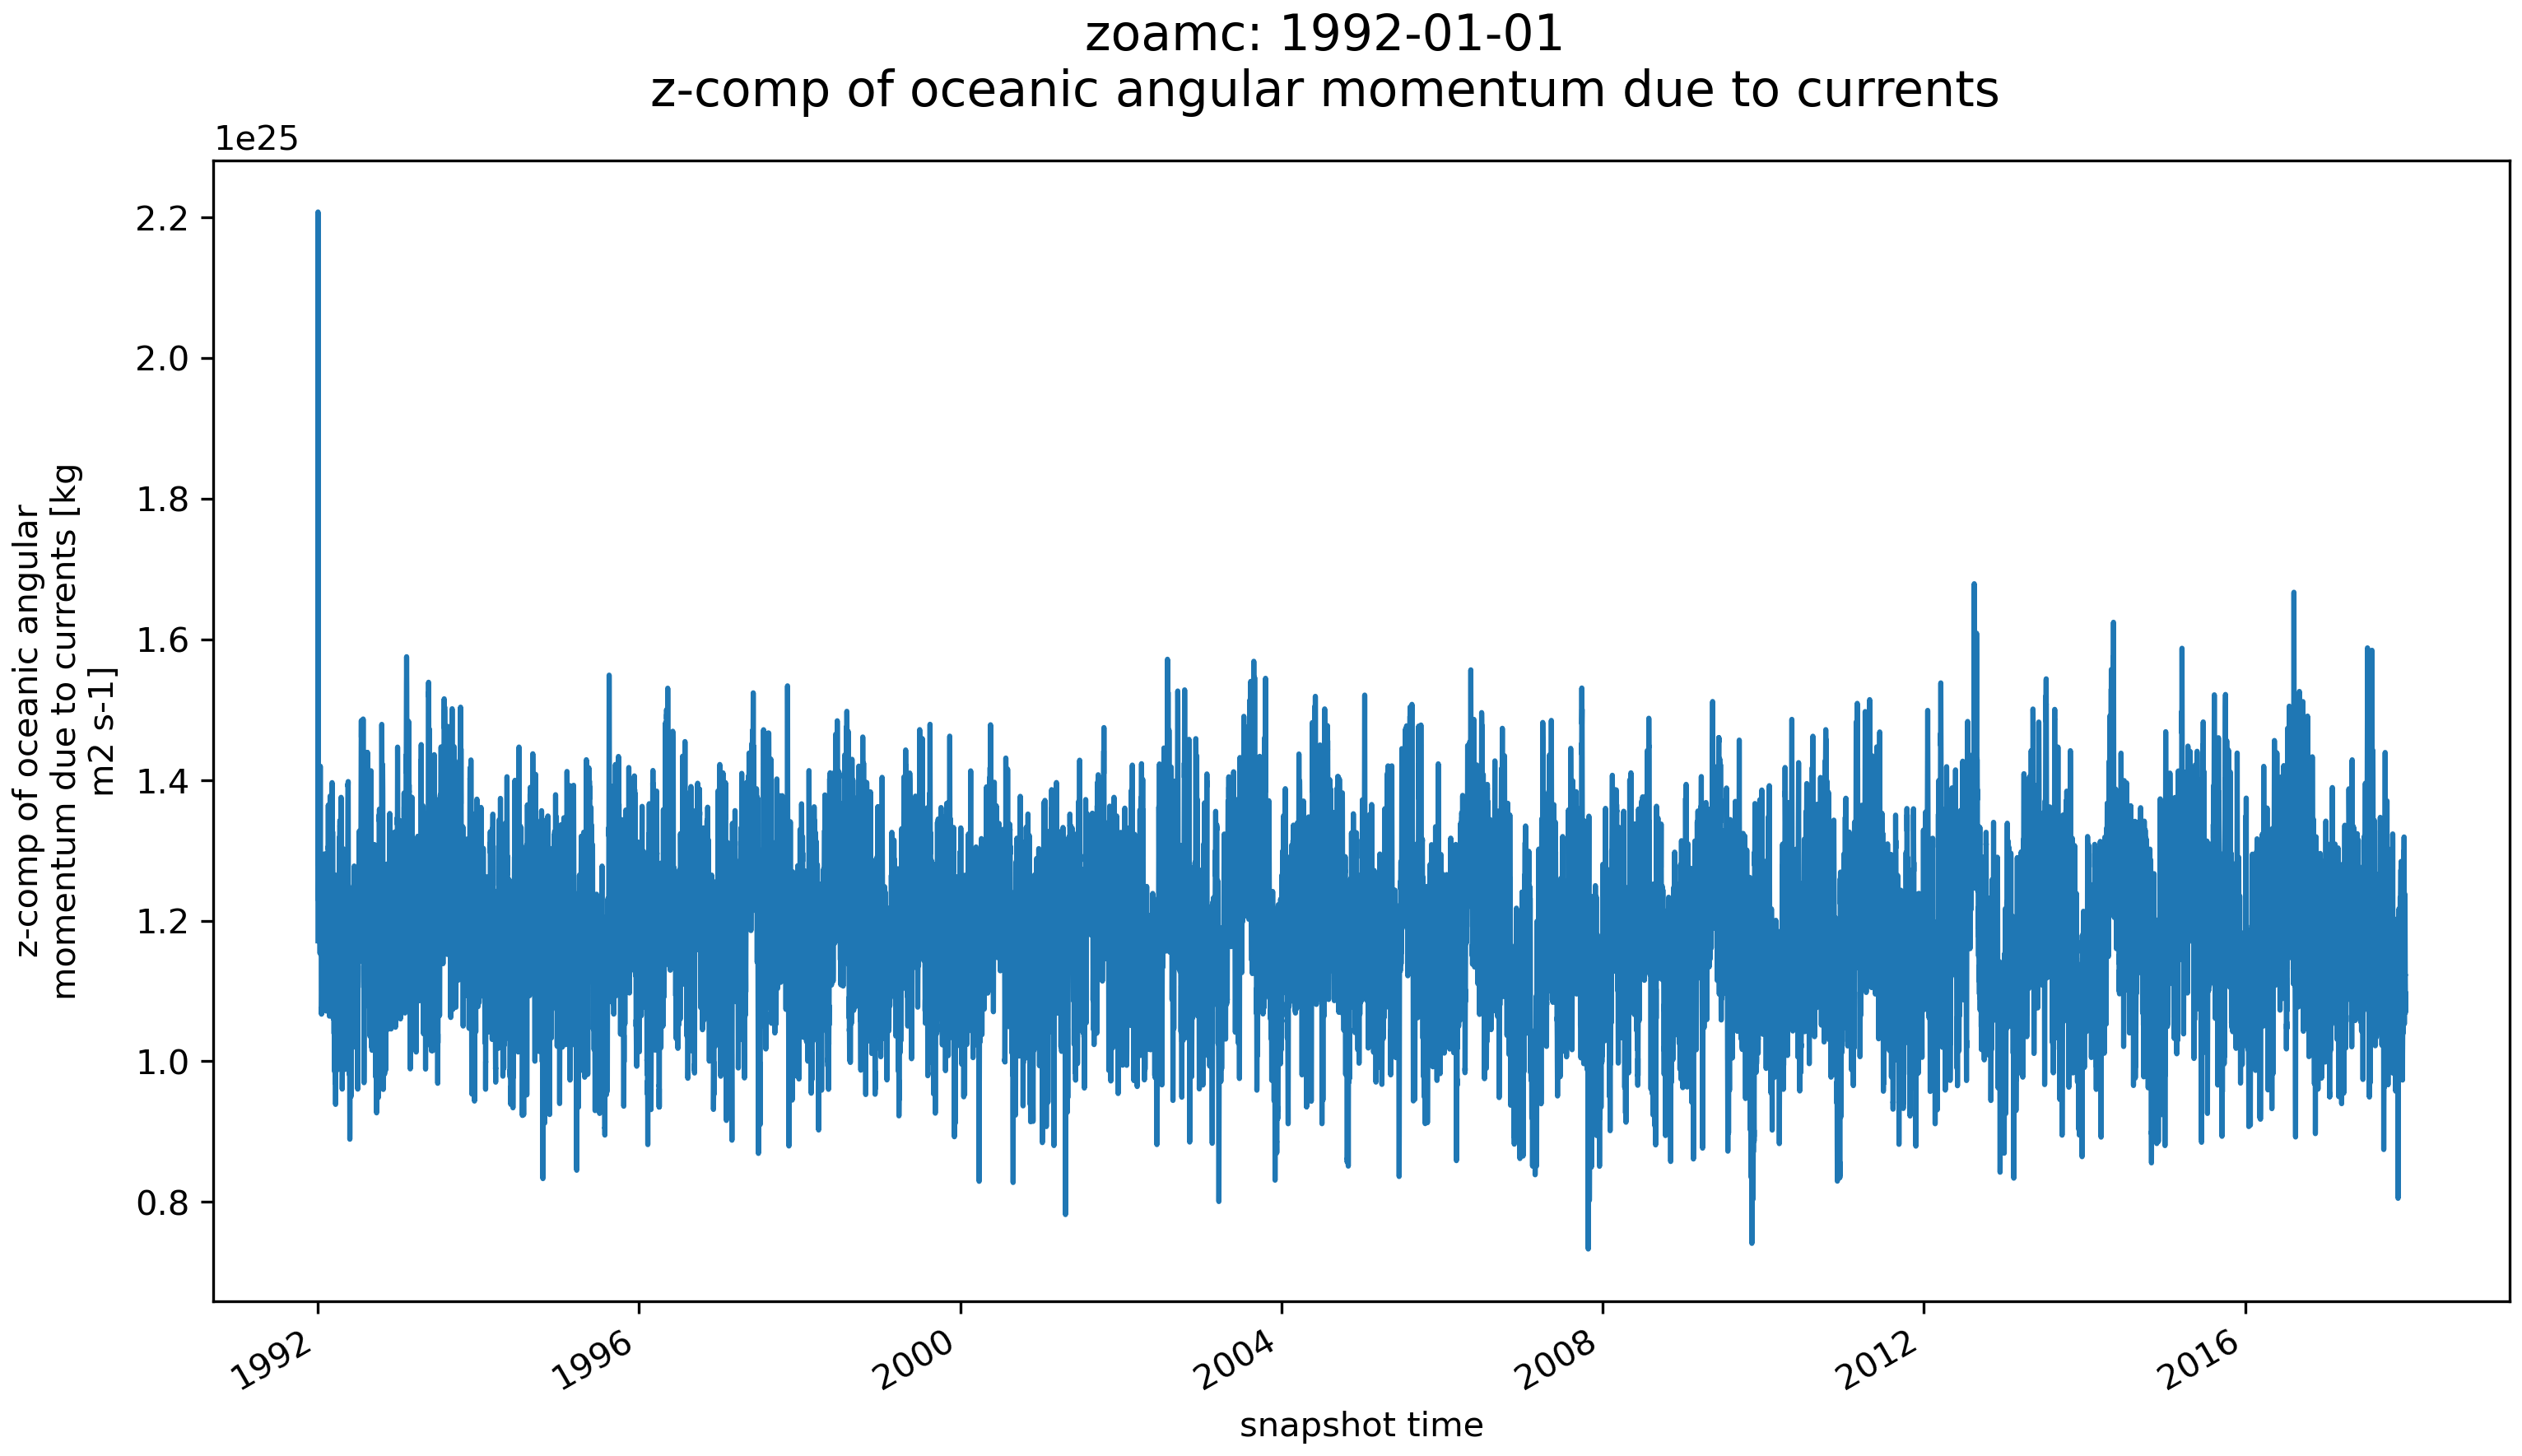
\includegraphics[scale=0.55]{../images/plots/oneD_plots/SBO_Core_Products/zoamc.png}
\caption{Dataset: SBO\_CORE\_PRODUCTS Variable: zoamc}
\label{tab:table-SBO_CORE_PRODUCTS_zoamc-Plot}
\end{figure}
\pagebreak
\subsubsection{1D Variable zoamc\_si}
\begin{longtable}{|m{0.06\textwidth}|m{0.41\textwidth}|m{0.39\textwidth}|m{0.06\textwidth}|}
\caption{CDL description of SBO\_CORE\_PRODUCTS's zoamc\_si variable}
\label{tab:table-SBO_CORE_PRODUCTS_zoamc_si} \\ 
\hline \endhead \hline \endfoot
\rowcolor{lightgray} \textbf{Storage Type} & \textbf{Variable Name} & \textbf{Description} & \textbf{Unit} \\ \hline
float64 & zoamc\_si & z-comp of oceanic angular momentum due to sea-ice motion & kg m2 s-1 \\ \hline
\rowcolor{lightgray}  \multicolumn{4}{|p{1.00\textwidth}|}{\textbf{CDL Description}} \\ \hline
\multicolumn{4}{|p{1.00\textwidth}|}{\makecell{\parbox{1\textwidth}{float64 zoamc\_si(time)\\
\hspace*{0.5cm}zoamc\_si: \_FillValue = 9.969209968386869e+36\\
\hspace*{0.5cm}zoamc\_si: coverage\_content\_type = modelResult\\
\hspace*{0.5cm}zoamc\_si: long\_name = z: comp of oceanic angular momentum due to sea: ice motion\\
\hspace*{0.5cm}zoamc\_si: units = kg m2 s: 1\\
\hspace*{0.5cm}zoamc\_si: valid\_min = : 5.909426721868294e+21\\
\hspace*{0.5cm}zoamc\_si: valid\_max = 5.930388258256482e+21\\
\hspace*{0.5cm}zoamc\_si: coordinates = time}}} \\ \hline
\rowcolor{lightgray} \multicolumn{4}{|p{1.00\textwidth}|}{\textbf{Comments}} \\ \hline
\multicolumn{4}{|p{1\textwidth}|}{N/A} \\ \hline
\end{longtable}

\begin{figure}[H]
\centering
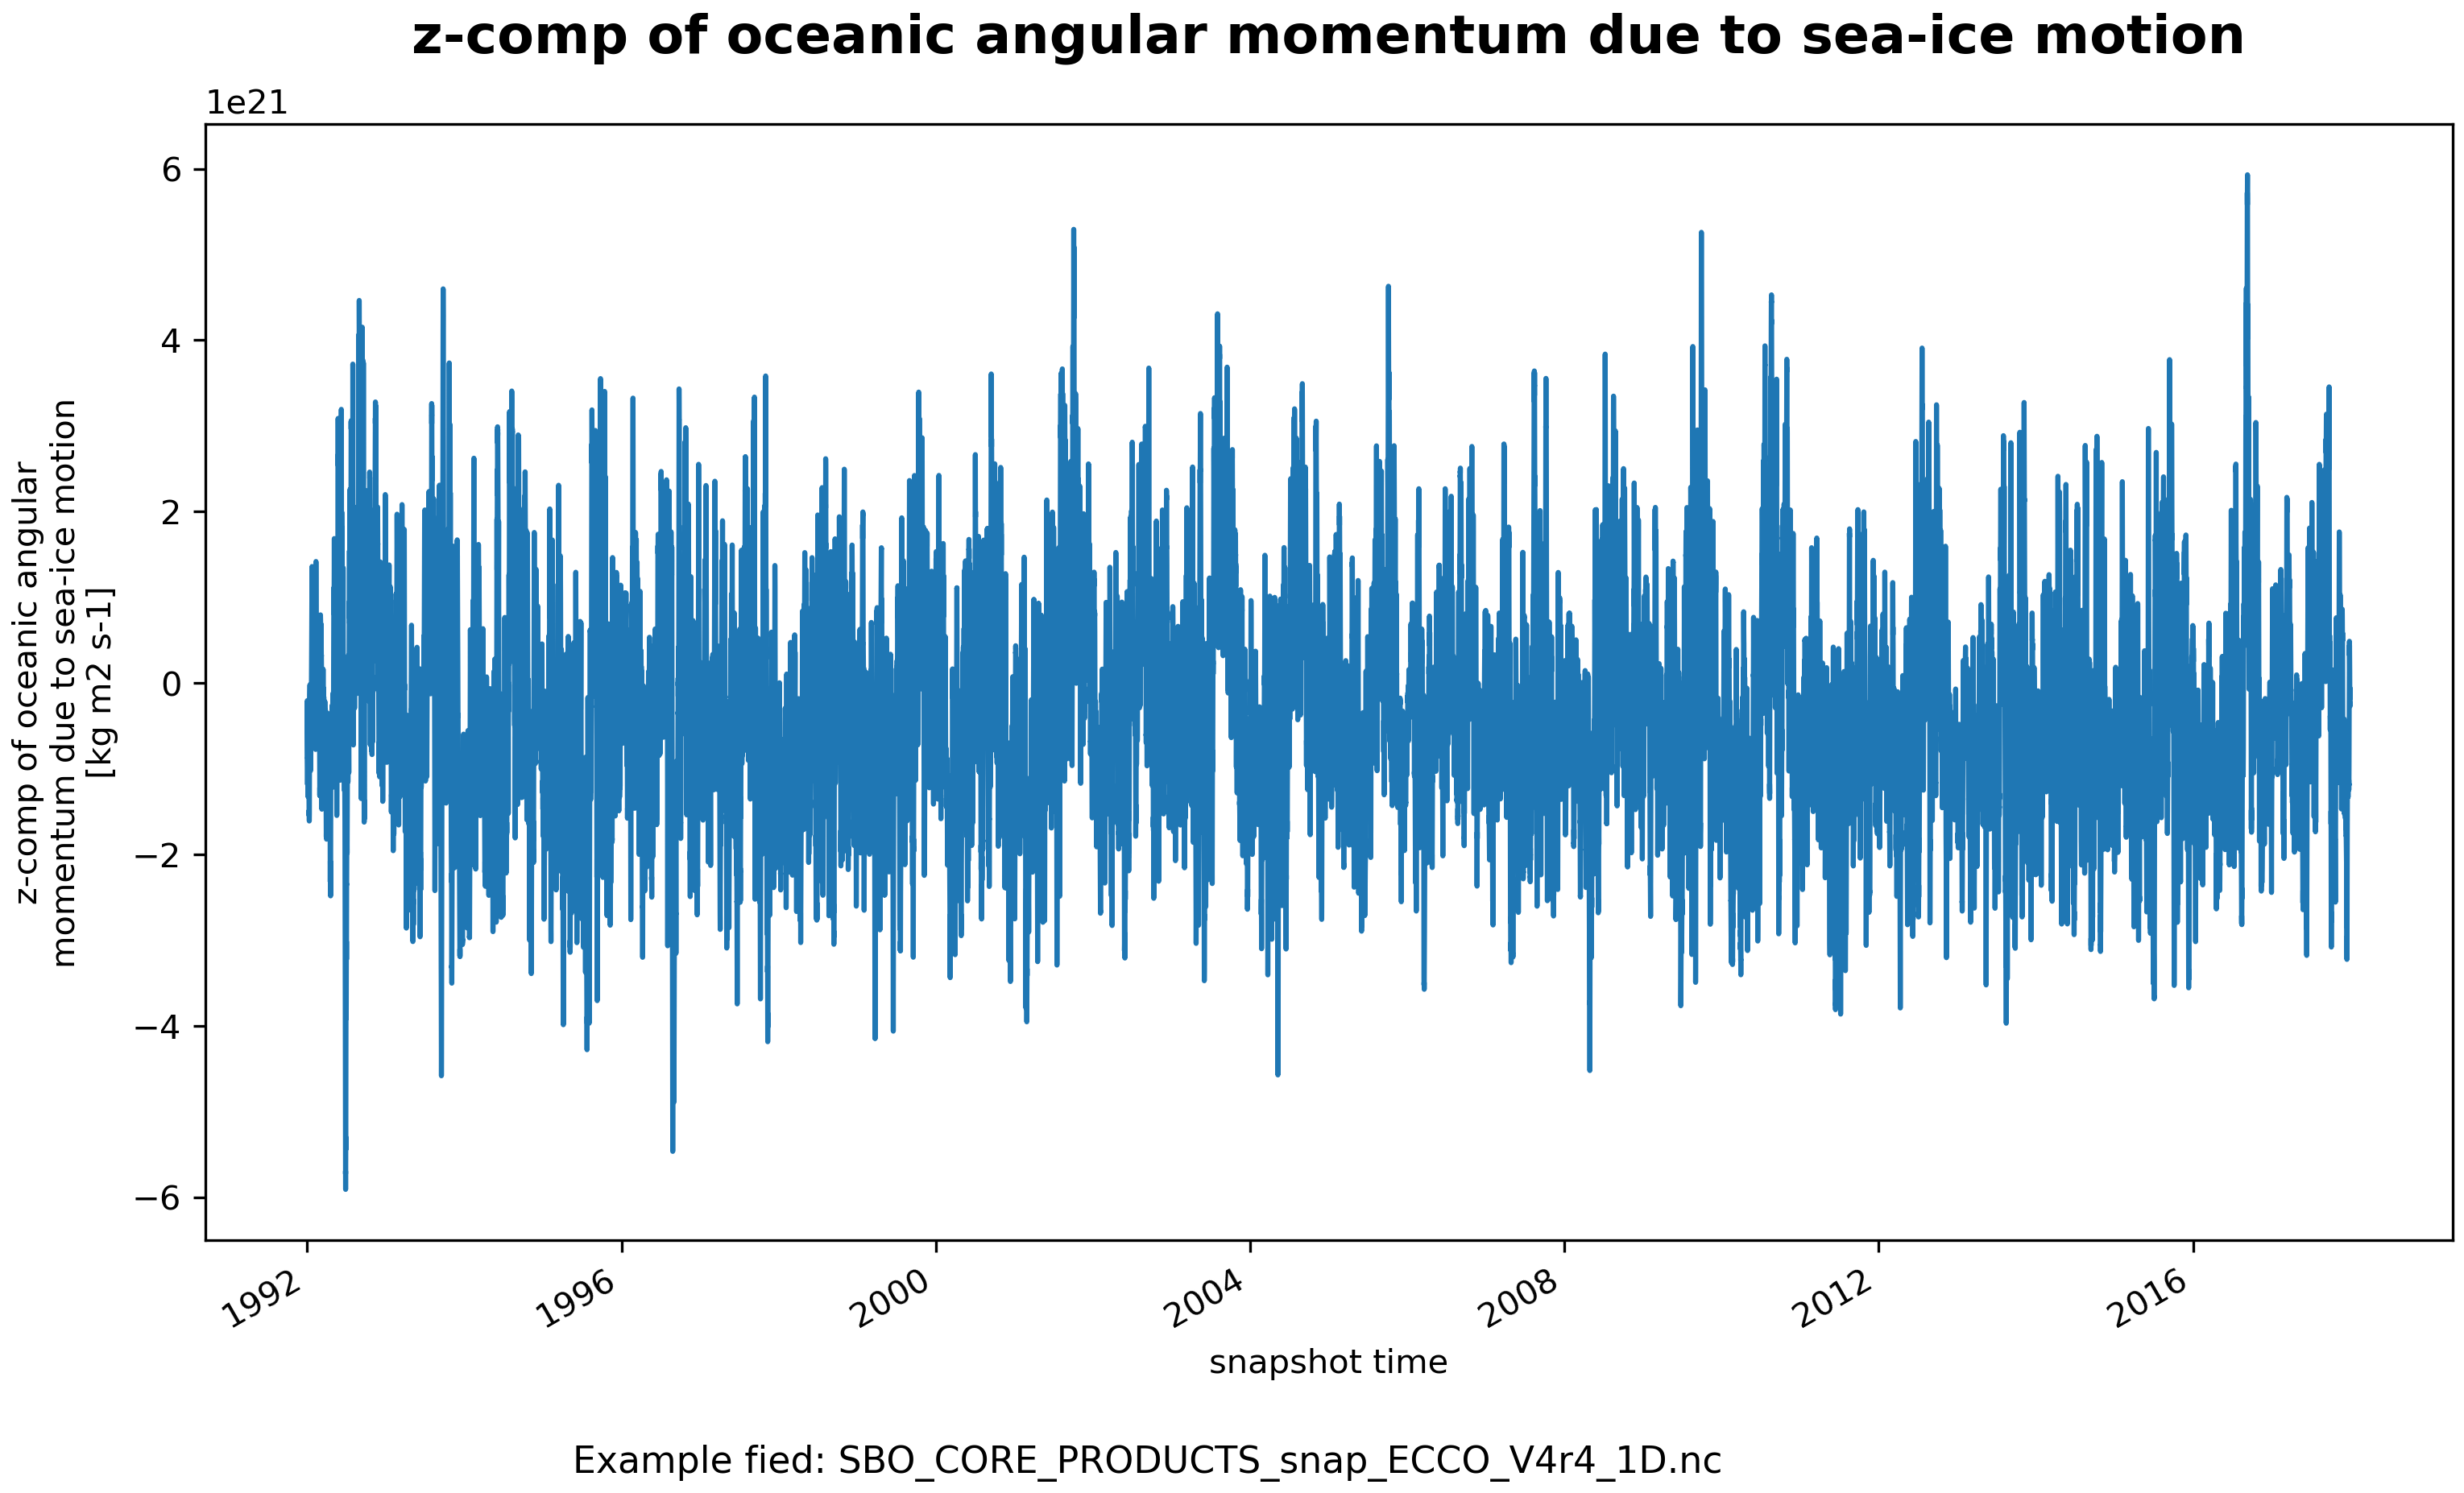
\includegraphics[scale=0.55]{../images/plots/oneD_plots/SBO_Core_Products/zoamc_si.png}
\caption{Dataset: SBO\_CORE\_PRODUCTS Variable: zoamc\_si}
\label{tab:table-SBO_CORE_PRODUCTS_zoamc_si-Plot}
\end{figure}
\pagebreak
\subsubsection{1D Variable zoamp}
\begin{longtable}{|m{0.06\textwidth}|m{0.41\textwidth}|m{0.39\textwidth}|m{0.06\textwidth}|}
\caption{CDL description of SBO\_CORE\_PRODUCTS's zoamp variable}
\label{tab:table-SBO_CORE_PRODUCTS_zoamp} \\ 
\hline \endhead \hline \endfoot
\rowcolor{lightgray} \textbf{Storage Type} & \textbf{Variable Name} & \textbf{Description} & \textbf{Unit} \\ \hline
float64 & zoamp & z-comp of oceanic angular momentum due to pressure & kg m2 s-1 \\ \hline
\rowcolor{lightgray}  \multicolumn{4}{|p{1.00\textwidth}|}{\textbf{CDL Description}} \\ \hline
\multicolumn{4}{|p{1.00\textwidth}|}{\makecell{\parbox{1\textwidth}{float64 zoamp(time)\\
\hspace*{0.5cm}zoamp: \_FillValue = 9.969209968386869e+36\\
\hspace*{0.5cm}zoamp: coverage\_content\_type = modelResult\\
\hspace*{0.5cm}zoamp: long\_name = z: comp of oceanic angular momentum due to pressure\\
\hspace*{0.5cm}zoamp: units = kg m2 s: 1\\
\hspace*{0.5cm}zoamp: valid\_min = 2.927645942668479e+30\\
\hspace*{0.5cm}zoamp: valid\_max = 2.9277200254389854e+30\\
\hspace*{0.5cm}zoamp: coordinates = time}}} \\ \hline
\rowcolor{lightgray} \multicolumn{4}{|p{1.00\textwidth}|}{\textbf{Comments}} \\ \hline
\multicolumn{4}{|p{1\textwidth}|}{N/A} \\ \hline
\end{longtable}

\begin{figure}[H]
\centering
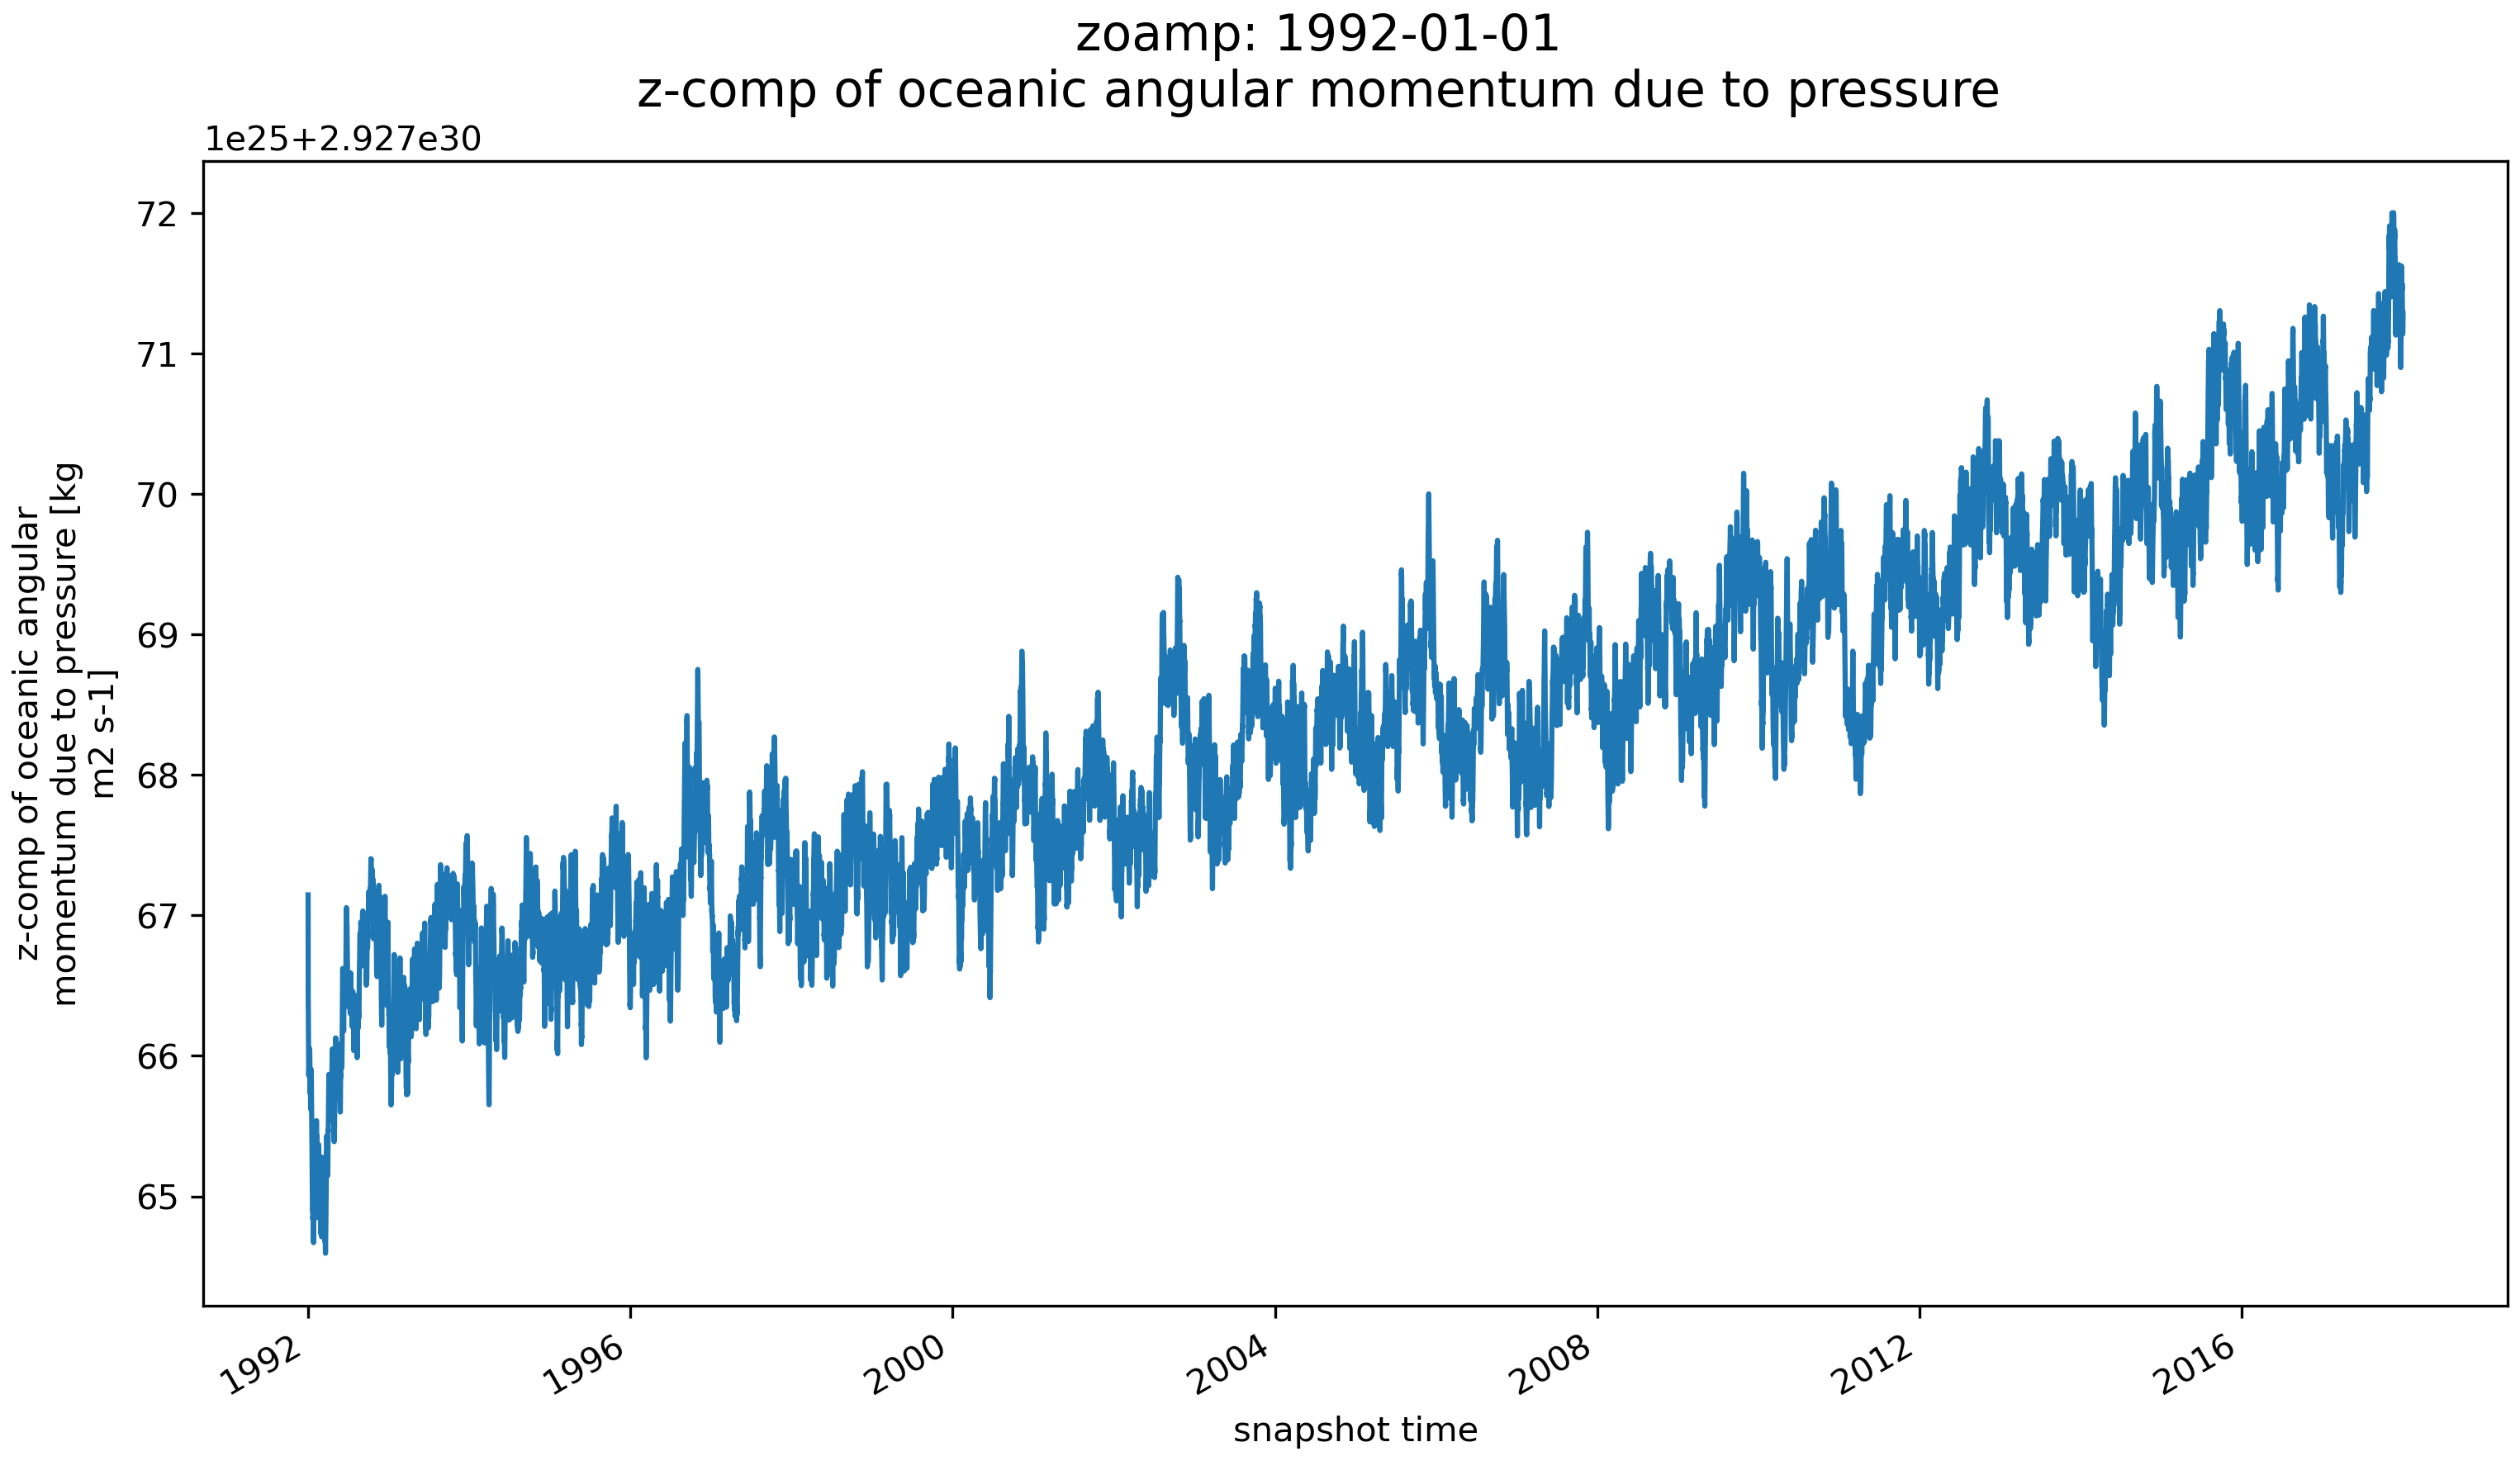
\includegraphics[scale=0.55]{../images/plots/oneD_plots/SBO_Core_Products/zoamp.png}
\caption{Dataset: SBO\_CORE\_PRODUCTS Variable: zoamp}
\label{tab:table-SBO_CORE_PRODUCTS_zoamp-Plot}
\end{figure}
\pagebreak
\subsubsection{1D Variable zoamp\_dsl}
\begin{longtable}{|m{0.06\textwidth}|m{0.41\textwidth}|m{0.39\textwidth}|m{0.06\textwidth}|}
\caption{CDL description of SBO\_CORE\_PRODUCTS's zoamp\_dsl variable}
\label{tab:table-SBO_CORE_PRODUCTS_zoamp_dsl} \\ 
\hline \endhead \hline \endfoot
\rowcolor{lightgray} \textbf{Storage Type} & \textbf{Variable Name} & \textbf{Description} & \textbf{Unit} \\ \hline
float64 & zoamp\_dsl & z-comp of oceanic angular momentum due to pressure based on dynamic (IB-corrected) sea level & kg m2 s-1 \\ \hline
\rowcolor{lightgray}  \multicolumn{4}{|p{1.00\textwidth}|}{\textbf{CDL Description}} \\ \hline
\multicolumn{4}{|p{1.00\textwidth}|}{\makecell{\parbox{1\textwidth}{float64 zoamp\_dsl(time)\\
\hspace*{0.5cm}zoamp\_dsl: \_FillValue = 9.969209968386869e+36\\
\hspace*{0.5cm}zoamp\_dsl: coverage\_content\_type = modelResult\\
\hspace*{0.5cm}zoamp\_dsl: long\_name = z: comp of oceanic angular momentum due to pressure based on dynamic (IB: corrected) sea level\\
\hspace*{0.5cm}zoamp\_dsl: units = kg m2 s: 1\\
\hspace*{0.5cm}zoamp\_dsl: valid\_min = 2.9276609546728614e+30\\
\hspace*{0.5cm}zoamp\_dsl: valid\_max = 2.9277328440911863e+30\\
\hspace*{0.5cm}zoamp\_dsl: coordinates = time}}} \\ \hline
\rowcolor{lightgray} \multicolumn{4}{|p{1.00\textwidth}|}{\textbf{Comments}} \\ \hline
\multicolumn{4}{|p{1\textwidth}|}{N/A} \\ \hline
\end{longtable}

\begin{figure}[H]
\centering
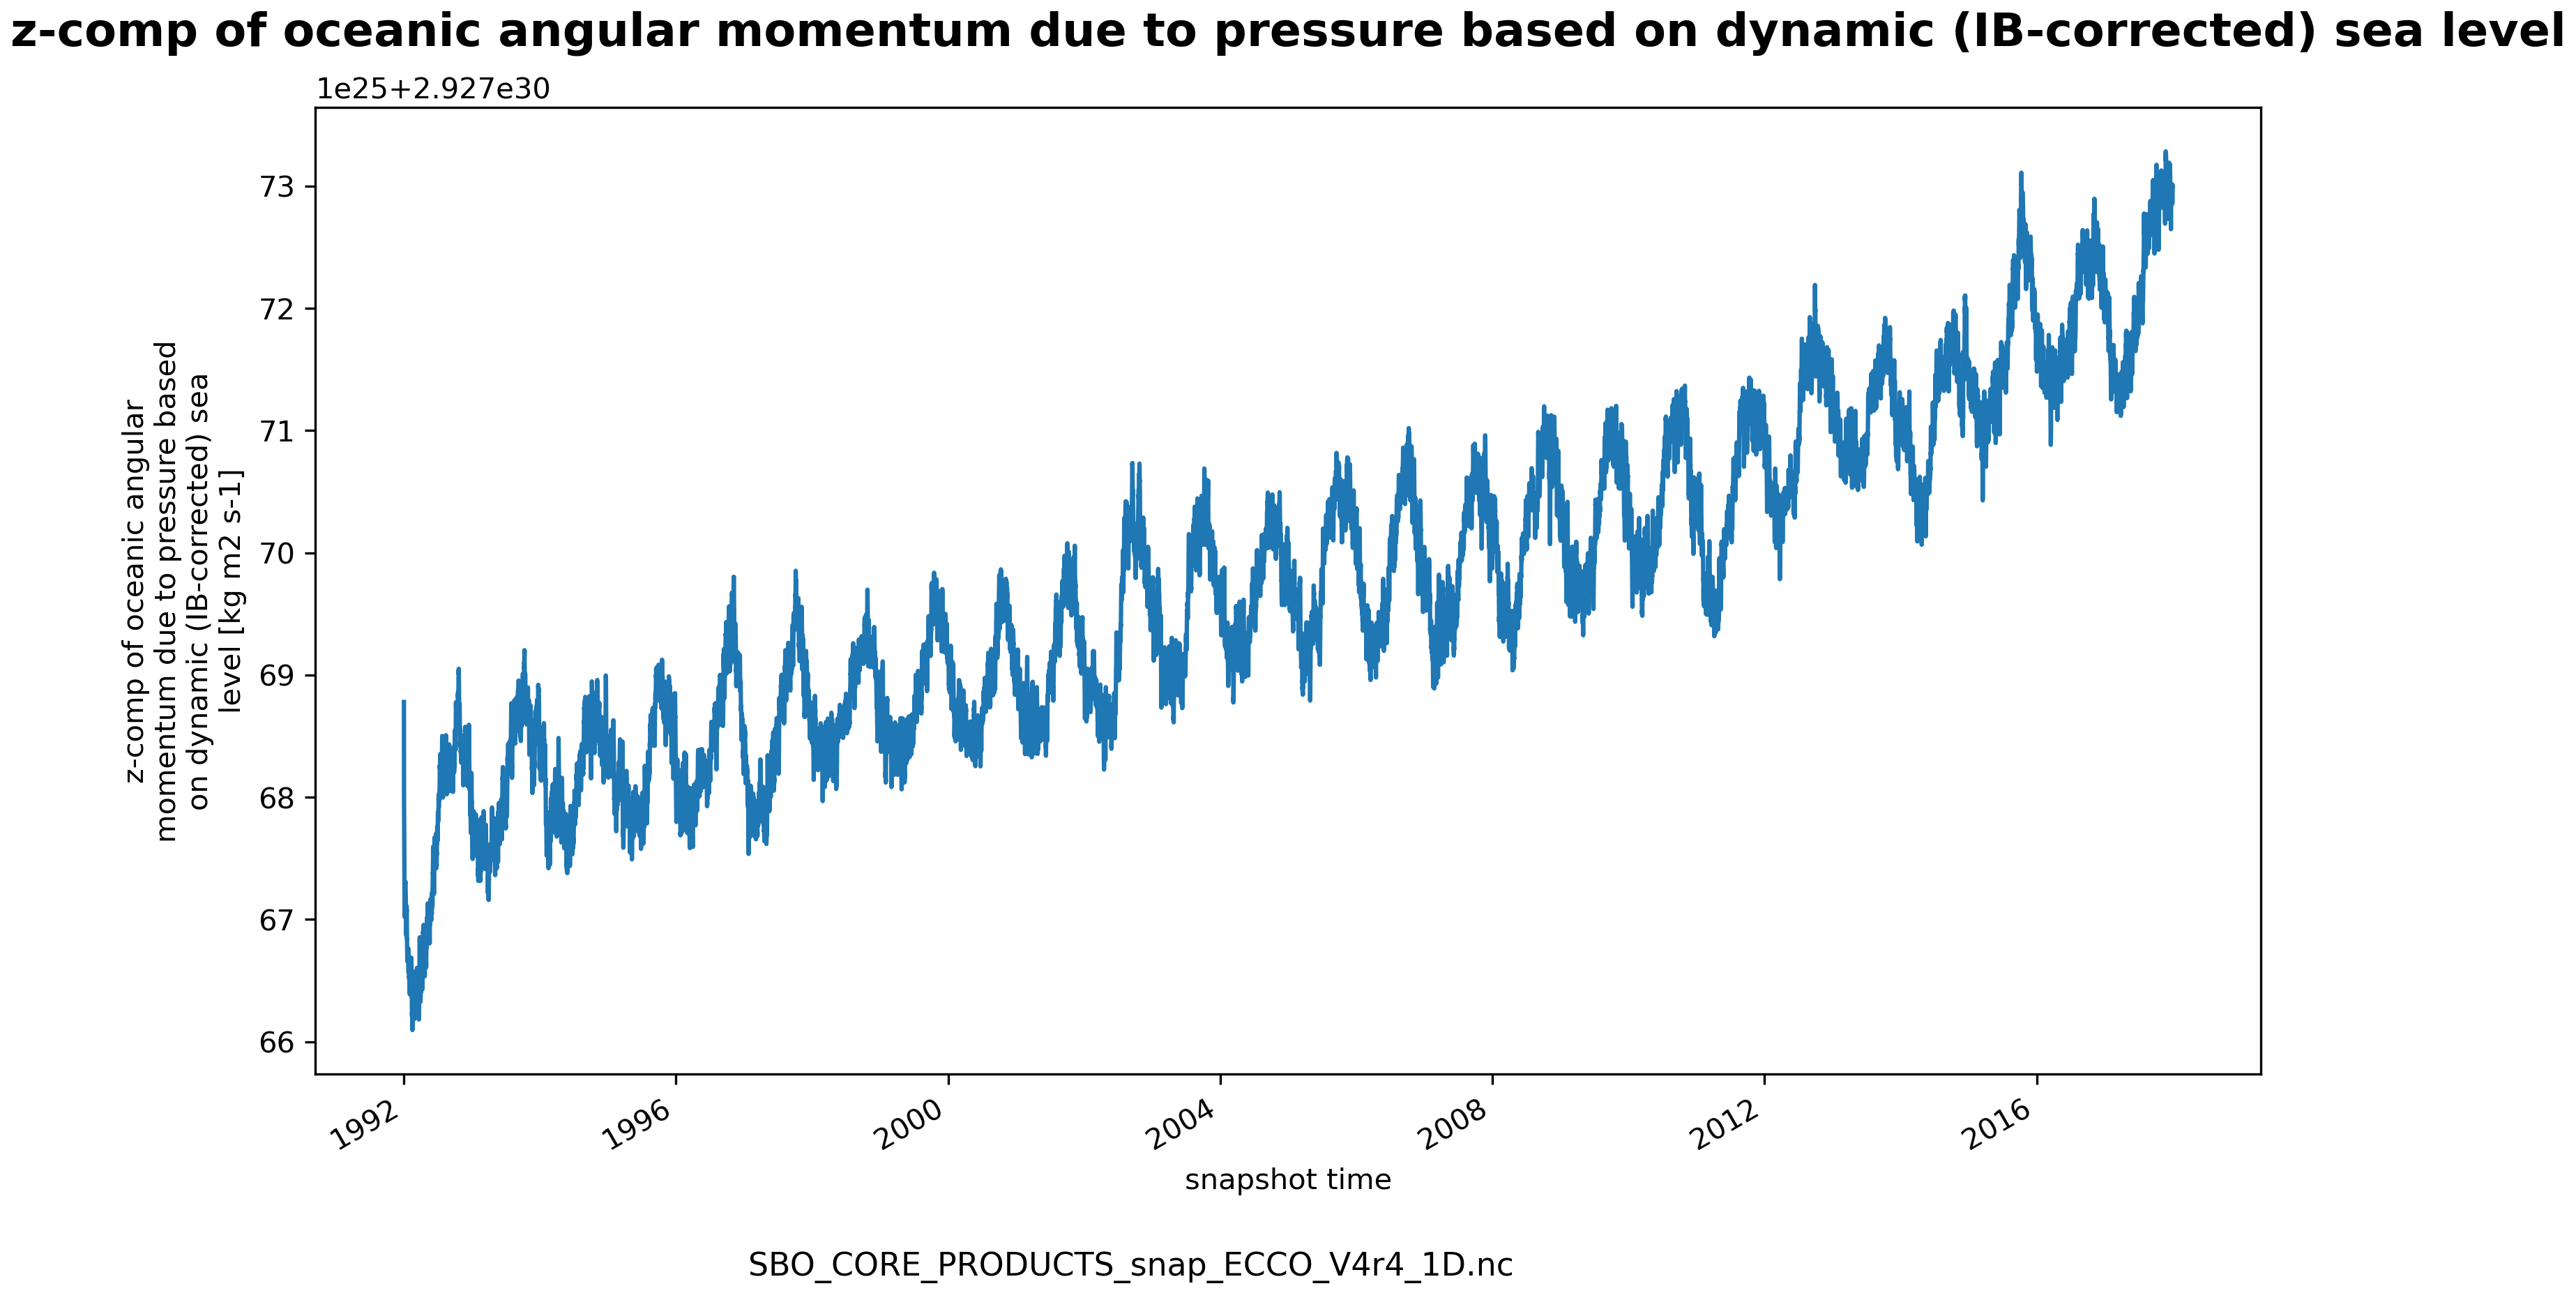
\includegraphics[scale=0.55]{../images/plots/oneD_plots/SBO_Core_Products/zoamp_dsl.png}
\caption{Dataset: SBO\_CORE\_PRODUCTS Variable: zoamp\_dsl}
\label{tab:table-SBO_CORE_PRODUCTS_zoamp_dsl-Plot}
\end{figure}
\pagebreak
\subsubsection{1D Variable zoamp\_fw}
\begin{longtable}{|m{0.06\textwidth}|m{0.41\textwidth}|m{0.39\textwidth}|m{0.06\textwidth}|}
\caption{CDL description of SBO\_CORE\_PRODUCTS's zoamp\_fw variable}
\label{tab:table-SBO_CORE_PRODUCTS_zoamp_fw} \\ 
\hline \endhead \hline \endfoot
\rowcolor{lightgray} \textbf{Storage Type} & \textbf{Variable Name} & \textbf{Description} & \textbf{Unit} \\ \hline
float64 & zoamp\_fw & z-comp of oceanic angular momentum due to freshwater flux & kg m2 s-1 \\ \hline
\rowcolor{lightgray}  \multicolumn{4}{|p{1.00\textwidth}|}{\textbf{CDL Description}} \\ \hline
\multicolumn{4}{|p{1.00\textwidth}|}{\makecell{\parbox{1\textwidth}{float64 zoamp\_fw(time)\\
\hspace*{0.5cm}zoamp\_fw: \_FillValue = 9.969209968386869e+36\\
\hspace*{0.5cm}zoamp\_fw: coverage\_content\_type = modelResult\\
\hspace*{0.5cm}zoamp\_fw: long\_name = z: comp of oceanic angular momentum due to freshwater flux\\
\hspace*{0.5cm}zoamp\_fw: units = kg m2 s: 1\\
\hspace*{0.5cm}zoamp\_fw: valid\_min = 7.774584605728723e+25\\
\hspace*{0.5cm}zoamp\_fw: valid\_max = 1.442874536478883e+26\\
\hspace*{0.5cm}zoamp\_fw: coordinates = time}}} \\ \hline
\rowcolor{lightgray} \multicolumn{4}{|p{1.00\textwidth}|}{\textbf{Comments}} \\ \hline
\multicolumn{4}{|p{1\textwidth}|}{N/A} \\ \hline
\end{longtable}

\begin{figure}[H]
\centering
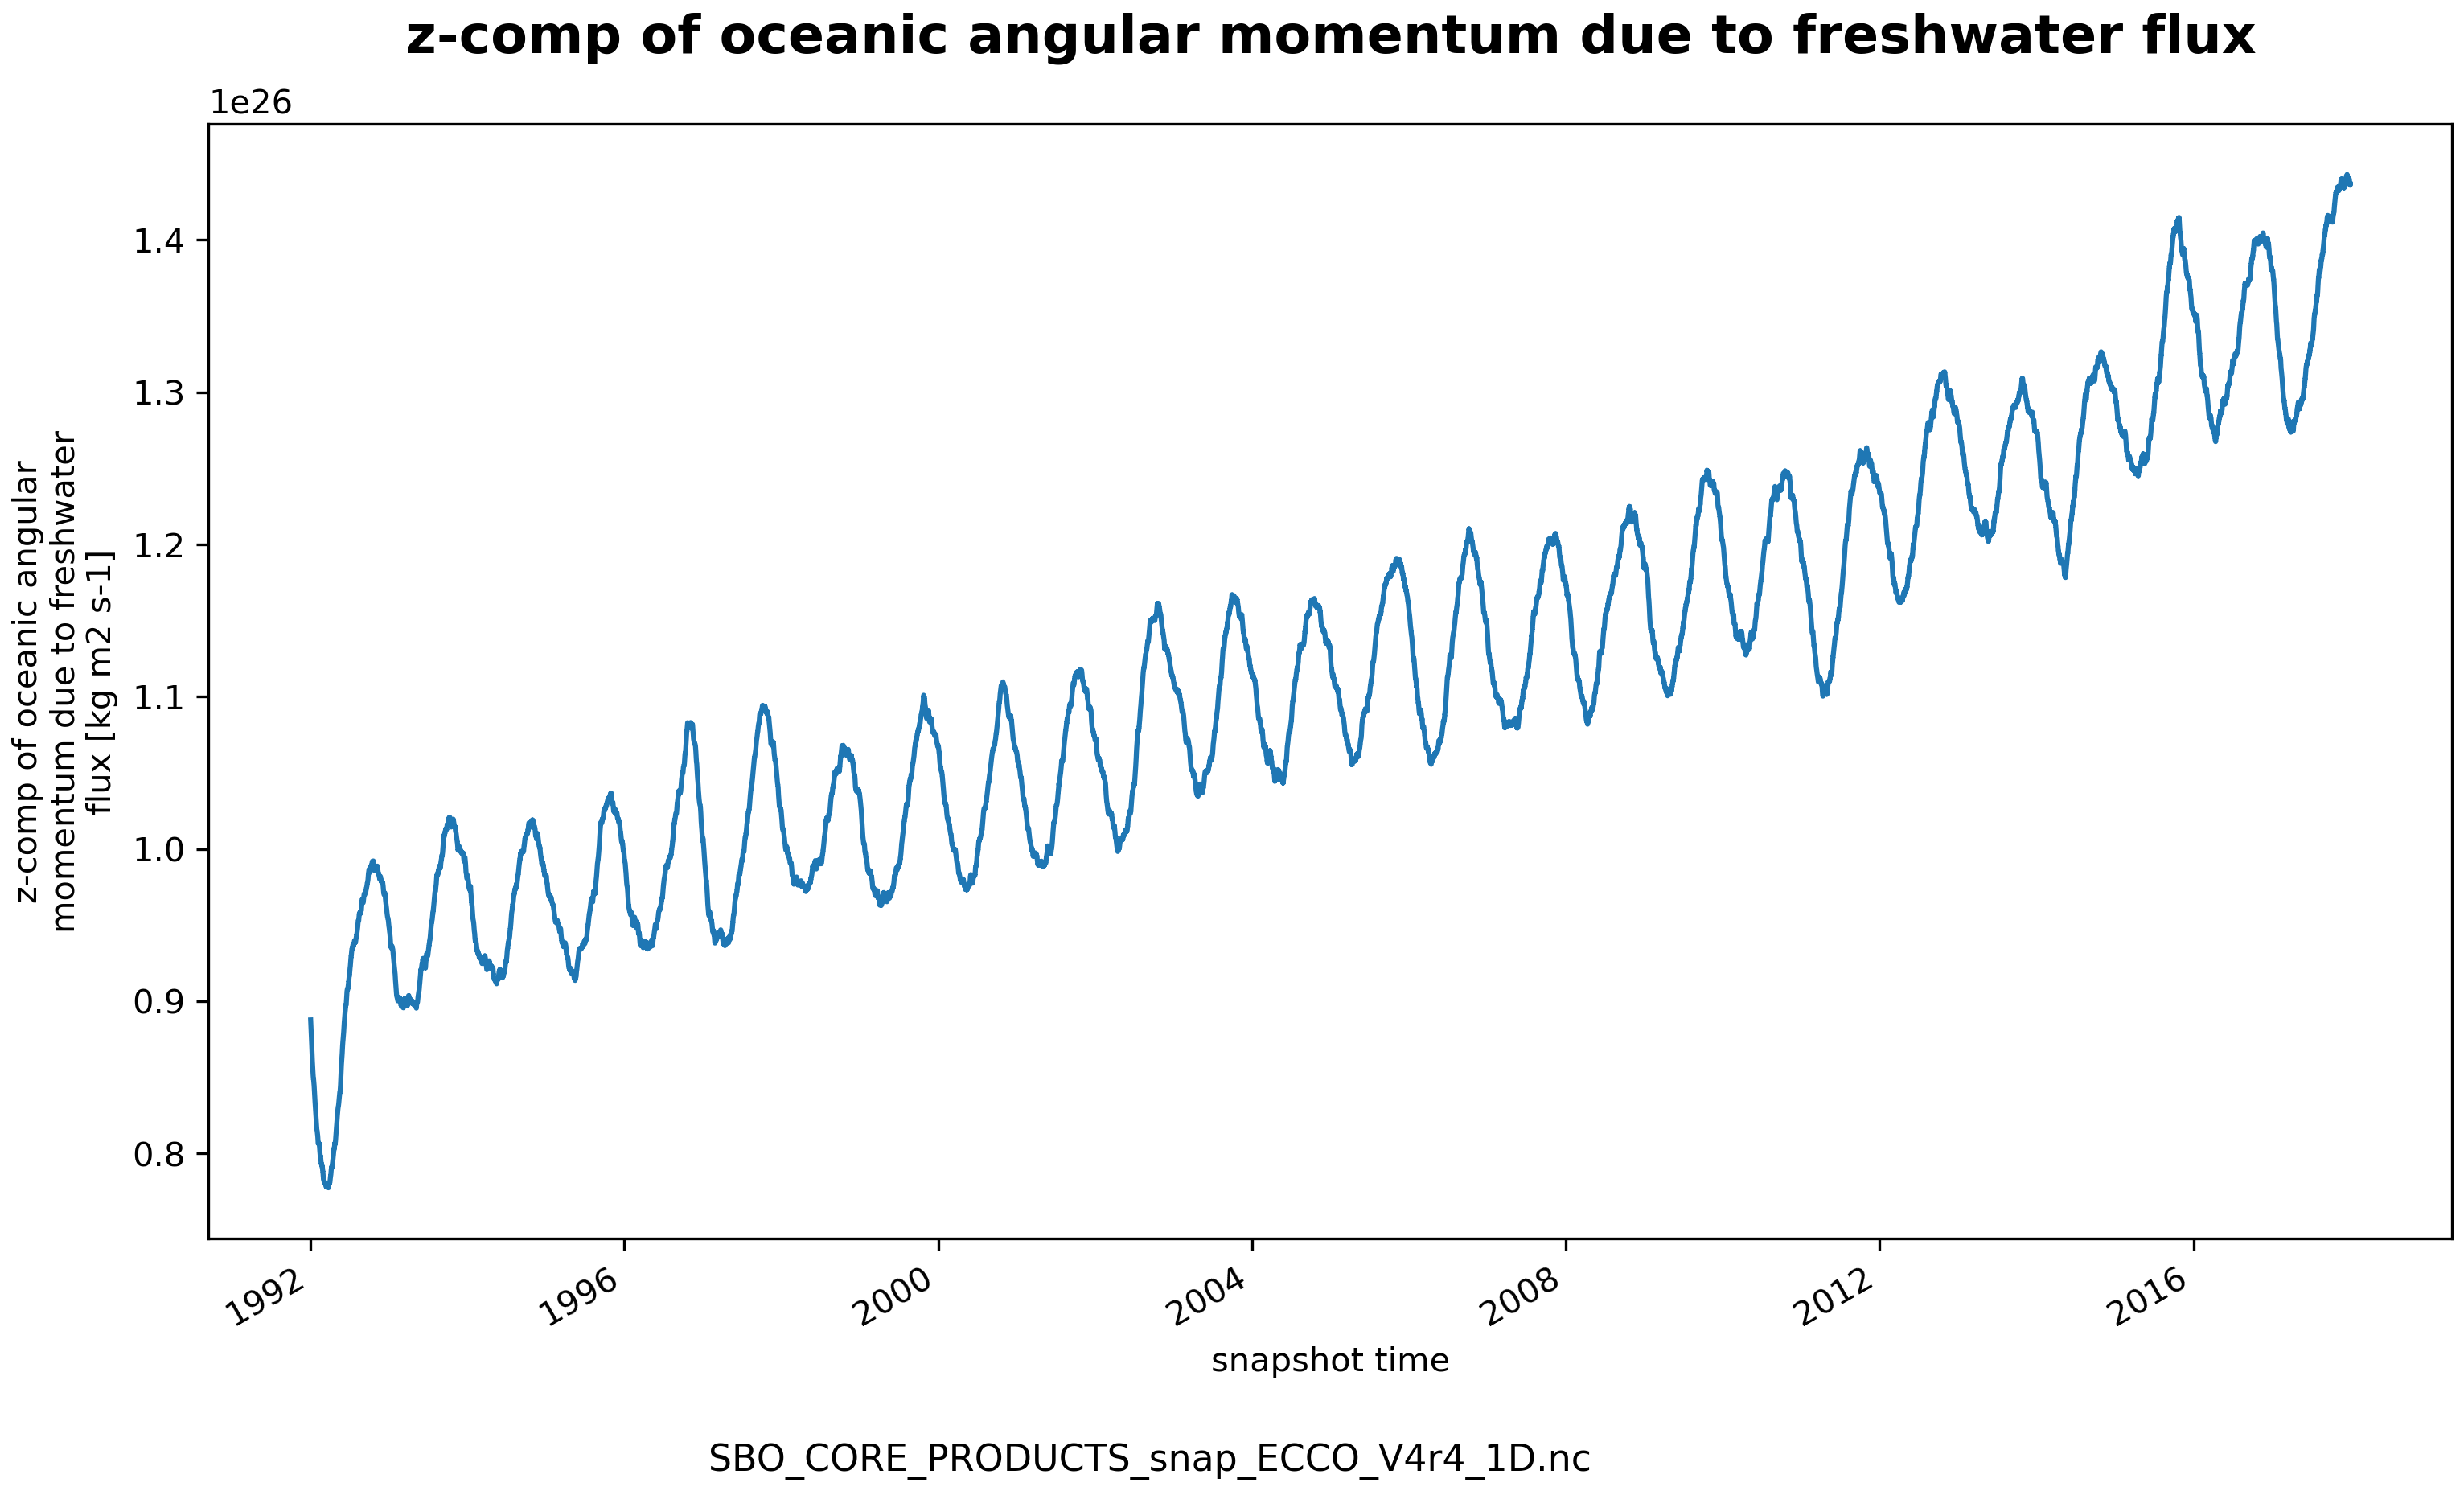
\includegraphics[scale=0.55]{../images/plots/oneD_plots/SBO_Core_Products/zoamp_fw.png}
\caption{Dataset: SBO\_CORE\_PRODUCTS Variable: zoamp\_fw}
\label{tab:table-SBO_CORE_PRODUCTS_zoamp_fw-Plot}
\end{figure}